%-------------------------------------------------------------------------------

% This file is part of code_saturne, a general-purpose CFD tool.
%
% Copyright (C) 1998-2022 EDF S.A.
%
% This program is free software; you can redistribute it and/or modify it under
% the terms of the GNU General Public License as published by the Free Software
% Foundation; either version 2 of the License, or (at your option) any later
% version.
%
% This program is distributed in the hope that it will be useful, but WITHOUT
% ANY WARRANTY; without even the implied warranty of MERCHANTABILITY or FITNESS
% FOR A PARTICULAR PURPOSE.  See the GNU General Public License for more
% details.
%
% You should have received a copy of the GNU General Public License along with
% this program; if not, write to the Free Software Foundation, Inc., 51 Franklin
% Street, Fifth Floor, Boston, MA 02110-1301, USA.

%-------------------------------------------------------------------------------

%%%%%%%%%%%%%%%%%%%%%%%%%%%%%%%%%%%%%%%%%%%%%%%%%%%%%%%%%%%%%%%%%%%%%%
% csdoc class wich is done for reports
\documentclass[a4paper,10pt,twoside]{csshortdoc}
% MACROS SUPPLEMENTAIRES
\usepackage{csmacros}
%
%%%%%%%%%%%%%%%%%%%%%%%%%%%%%%%%%%%%%%%%%%%%%%%%%%%%%%%%%%%%%%%%%%%%%%

%
%%%%%%%%%%%%%%%%%%%%%%%%%%%%%%%%%%%%%%%%%%%%%%%%%%%%%%%%%%%%%%%%%%%%%%
% PACKAGES ET COMMANDES POUR LE DOCUMENTS PDF ET LES HYPERLIENS
\hypersetup{%
  pdftitle = {CodeSaturne practical user's guide},
  pdfauthor = {MFEE},
  pdfpagemode = UseOutlines
}
\pdfinfo{/CreationDate (D:20030429000000-01 00 )}
%
% To have thumbnails upon opening the document under ACROREAD
% pdfpagemode = UseThumbs
%
%%%%%%%%%%%%%%%%%%%%%%%%%%%%%%%%%%%%%%%%%%%%%%%%%%%%%%%%%%%%%%%%%%%%%%
% REALISATION D'UN INDEX
\usepackage{makeidx}
\makeindex
%
%%%%%%%%%%%%%%%%%%%%%%%%%%%%%%%%%%%%%%%%%%%%%%%%%%%%%%%%%%%%%%%%%%%%%%
% PACKAGES ALLTT D'ENVIRONNEMENT VERBATIM AMELIORE
\usepackage{alltt}
%
%%%%%%%%%%%%%%%%%%%%%%%%%%%%%%%%%%%%%%%%%%%%%%%%%%%%%%%%%%%%%%%%%%%%%%
% INFO POUR PAGES DE GARDES
\titreCS{\CS version~\verscs practical user's guide}
\docassociesCS{}
\resumeCS{This document presents all the necessary elements to run a calculation
with \CS version \verscs. It then lists all the variables of the code
which may be useful for more advanced utilisation.
The user subroutines of all the modules within the code are also documented.
Eventually, for each key word and user-modifiable parameter in the code,
their definition, allowed values, default values and conditions for use are given.
These key words and parameters are grouped under headings
based on their function. An alphabetical index list is also given at the end of
the document for easier consultation.}
%
%%%%%%%%%%%%%%%%%%%%%%%%%%%%%%%%%%%%%%%%%%%%%%%%%%%%%%%%%%%%%%%%%%%%%%
% DEBUT DU DOCUMENT
\begin{document}

\def\contentsname{\textbf{\normalsize TABLE OF CONTENTS}\pdfbookmark[1]{Table of
contents}{contents}}
\def\indexname{Index of the main variables and keywords}

\renewcommand{\logocs}{cs_logo_h}

\pdfbookmark[1]{Flyleaf}{pdg}
\large
\makepdgCS
\normalsize

\input summary

\passepage

\begin{center}\begin{singlespace}
\tableofcontents
\end{singlespace}\end{center}
%
%%%%%%%%%%%%%%%%%%%%%%%%%%%%%%%%%%%%%%%%%%%%%%%%%%%%%%%%%%%%%%%%%%%%%%
% CORPS DU DOCUMENT
%
\passepage
%-------------------------------------------------------------------------------

% This file is part of code_saturne, a general-purpose CFD tool.
%
% Copyright (C) 1998-2022 EDF S.A.
%
% This program is free software; you can redistribute it and/or modify it under
% the terms of the GNU General Public License as published by the Free Software
% Foundation; either version 2 of the License, or (at your option) any later
% version.
%
% This program is distributed in the hope that it will be useful, but WITHOUT
% ANY WARRANTY; without even the implied warranty of MERCHANTABILITY or FITNESS
% FOR A PARTICULAR PURPOSE.  See the GNU General Public License for more
% details.
%
% You should have received a copy of the GNU General Public License along with
% this program; if not, write to the Free Software Foundation, Inc., 51 Franklin
% Street, Fifth Floor, Boston, MA 02110-1301, USA.

%-------------------------------------------------------------------------------

\nopagebreak
%==================================
%==================================
\section{Introduction}
%==================================
%==================================

This document is a practical user guide for \CS version \verscs.
It is the result of the joint effort of
all the members in the development team.

This document provides practical information for the usage of \CS.
For more details about the algorithms and their numerical implementation,
please refer to the reports
 \cite{ijvf}, and \cite{mechitoua98},
and to the theoretical documentation \cite{theory}.

The latest updated version of this document is available on-line with the version of \CS
and accessible through the command
\texttt{code\_saturne info --guide theory}.

This document presents some the necessary elements to run a calculation
with \CS version \verscs. It then lists all the variables of the code
which may be useful for more advanced users.
The user subroutines of all the modules within the code are then documented.
Eventually, for each keyword and user-modifiable parameter in the code,
their definition, allowed values, default values and conditions for use are given.
These keywords and parameters are grouped under headings
based on their function. An alphabetical index is also given at the end of
the document for easier reference.

In addition to the present user guide, a complete
\texttt{Doxygen} documentation is available with \CS. It can provide
information about the implementation such as details on variables used
throughout the solver and the user subroutines. It also provides an easily
explorable set of user subroutine examples and Fortran-C naming references for
quantities linked to the mesh or the physical fields.

The user documentation is in the process of migration from this pdf documentation
to the Doxygen documentation, so the user should first lok there.
One can access the \texttt{Doxygen} main page through \doxygenfile{index.html}{this link} or from a terminal by typing the following command:
\texttt{code\_saturne info --guide theory}.

%==================================
\section{Basic modelling setup}
%==================================

%==================================
\subsection{Manage boundary conditions}
%==================================

\texttt{cs\_user\_boundary\_conditions} is the second compulsory subroutine for every calculation launched
without interface (except in the case of specific physics where the
corresponding boundary condition user subroutine must be used).

When using the interface, only complex boundary conditions (input profiles, conditions varying in time, ...)
need to be defined with \texttt{cs\_user\_boundary\_conditions}.
In the case of a calculation launched without the
interface, all the boundary conditions must appear in \texttt{cs\_user\_boundary\_conditions}.

\texttt{cs\_user\_boundary\_conditions} is essentially constituted of loops on boundary
face subsets. Several sequences
of \verb+call getfbr+ \verb+('criterion', nlelt, lstelt)+ (cf.
\S\ref{sec:fvm_selector}) allow selecting
the boundary faces with respect to their group(s), their
color(s) or geometric criteria. If needed, geometric and
physical variables are also available to the user. These allow him
to select the boundary faces using other criteria.

For more details about the treatment of boundary conditions, the user
may refer to the theoretical and computer documentation \cite{theory} of
the subroutine \texttt{condli} (for wall conditions, see
\texttt{clptur}) (to access this document on a workstation, use
\mbox{\texttt{code\_saturne~info --guide theory}}).

From the user point of view, the boundary conditions are fully
defined by three arrays\footnote{Except with Lagrangian boundary condition}:
\texttt{itypfb(nfabor)}\index{\texttt{itypfb}},
\texttt{icodcl(nfabor,nvar)}\index{\texttt{icodcl}} and
\texttt{rcodcl(nfabor,nvar,3)}\index{\texttt{rcodcl}}.
\begin{list}{-}{}
\item \texttt{itypfb(ifac)} defines the type of the face \texttt{ifac}
      (input, wall, ...).
\item \texttt{icodcl(ifac,ivar)} defines the type of boundary
      condition for the variable \texttt{ivar} on the face \texttt{ifac}
      (Dirichlet, flux ...).
\item \texttt{rcodcl(ifac,ivar,.)} gives the numerical values associated with the
      type of boundary condition (value of the Dirichlet condition, of the flux ...).
\end{list}

In the case of standard boundary conditions (see
\S\ref{sec:prg_clstandard}), it is sufficient to complete \texttt{itypfb(ifac)} and
parts of the array \texttt{rcodcl}; the array \texttt{icodcl} and most of \texttt{rcodcl} are filled automatically. For non-standard boundary
conditions (see \S\ref{sec:prg_clnonstandard}), the arrays \texttt{icodcl} and
\texttt{rcodcl} must be fully completed.

%==================================
\subsubsection{Coding of standard boundary conditions}
%==================================
\label{sec:prg_clstandard}%
The standard keywords used by the indicator \texttt{itypfb} are:
\texttt{ientre\index{ientre}}, \texttt{iparoi\index{iparoi}},
\texttt{iparug\index{iparug}}, \texttt{isymet\index{isymet}},
\texttt{isolib\index{isolib}}, \texttt{ifrent\index{ifrent}}, \texttt{ifresf\index{ifresf}},
\texttt{i\_convective\_inlet\index{i\_convective\_inlet}} and \texttt{iindef\index{iindef}}.

\begin{list}{$\bullet$}{}
\item If \texttt{itypfb=ientre}: inlet face.

\begin{list}{$\rightarrow$}{}
\item Zero-flux condition for pressure and Dirichlet condition for all
      other variables. The value of the Dirichlet condition must be given in
      \texttt{rcodcl(ifac,ivar,1)} for every value of \texttt{ivar}, except for
      \texttt{ivar=ipr}. The other values of \texttt{rcodcl} and
      \texttt{icodcl} are filled automatically.
\end{list}

\item If \texttt{itypfb=iparoi}: smooth solid wall face, impermeable and with friction.

\begin{list}{$\rightarrow$}{}
\item the eventual sliding wall velocity of the face is
      found in \texttt{rcodcl(ifac,ivar,1)} (\texttt{ivar} being
      \texttt{iu}, \texttt{iv} or \texttt{iw}). The initial
      values of \texttt{rcodcl(ifac,ivar,1)} are zero for
      the three velocity components (and therefore are to be specified
      only if the velocity is not equal to zero). \\
{\em WARNING: the wall sliding velocity must belong to the boundary face
      plane. For safety, the code only uses the projection of this
      velocity on the face. As a consequence, if the velocity specified
      by the user does not belong to the face plane, the wall sliding velocity really
      taken into account will be different.}

\item For scalars, two kinds of boundary conditions can be
      defined:
\begin{list}{$\rightsquigarrow$}{}
\item Imposed value at the wall. The user must write\\
\hspace*{1cm}\texttt{icodcl(ifac,ivar)}=5\\
\hspace*{1cm}\texttt{rcodcl(ifac,ivar,1)}=imposed value\\
\item Imposed flux at the wall. The user must write\\
\hspace*{1cm}\texttt{icodcl(ifac,ivar)}=3\\
\hspace*{1cm}\texttt{rcodcl(ifac,ivar,3)}=imposed flux value (depending on the
variable, the user may refer to the case \texttt{icodcl}=3 of \S~\ref{sec:prg_clnonstandard} for the flux definition).
\item If the user does not fill these arrays, the default condition
      is zero flux.
\end{list}
\end{list}

\item If \texttt{itypfb=iparug}: rough solid wall face, impermeable and with friction.

\begin{list}{$\rightarrow$}{}
\item the eventual moving velocity of the wall tangent to the face is
      given by \texttt{rcodcl(ifac,ivar,1)} (\texttt{ivar} being
      \texttt{iu}, \texttt{iv} or \texttt{iw}). The initial
      value of \texttt{rcodcl(ifac,ivar,1)} is zero for
      the three velocity components (and therefore must be specified
      only in the case of the existence of a slipping velocity). \\
{\em WARNING: the wall moving velocity must be in the boundary face
      plane. By security, the code uses only the projection of this
      velocity on the face. As a consequence, if the velocity specified
      by the user is not in the face plane, the wall moving velocity really
      taken into account will be different.}
\item The dynamic roughness must be specified in \texttt{rcodcl(ifac,iu,3)}.
      The values of \texttt{rcodcl(ifac,iv,3)} stores the thermal and scalar roughness.
      The values of \texttt{rcodcl(ifac,iw,3)} is not used.
\item For scalars, two kinds of boundary conditions can be defined:
\begin{list}{$\rightsquigarrow$}{}
\item Imposed value at the wall. The user must write\\
\hspace*{1cm}\texttt{icodcl(ifac,ivar)}=6\\
\hspace*{1cm}\texttt{rcodcl(ifac,ivar,1)}=imposed value\\
\item Imposed flux at the wall. The user must write\\
\hspace*{1cm}\texttt{icodcl(ifac,ivar)}=3\\
\hspace*{1cm}\texttt{rcodcl(ifac,ivar,3)}= imposed flux value (definition
      of the flux condition according to the variable, the user can refer to the
      case \texttt{icodcl}=3 of the paragraph \ref{sec:prg_clnonstandard}).
\item If the user does not complete these arrays, the default condition
      is zero flux.
\end{list}
\end{list}
\item If \texttt{itypfb=isymet}: symmetry face (or wall without friction).
\begin{list}{$\rightarrow$}{}
\item Nothing to be writen in \texttt{icodcl} and  \texttt{rcodcl}.
\end{list}

\item If \texttt{itypfb=isolib}: free outlet face (or more precisely free
      inlet/outlet with forced pressure)
\begin{list}{$\rightarrow$}{}
\item The pressure is always treated with a Dirichlet condition, calculated
      with the constraint $\displaystyle \frac{\partial }{\partial n}\left(\frac{ \partial P}{\partial \tau}\right)=0$.
      The pressure is set to $P_0$ at the first \texttt{isolib} face met.
      The pressure calibration is always done on a single face, even if there are
      several outlets.
\item If the mass flow is coming in, the velocity is set to zero
      and a Dirichlet condition for the scalars and the turbulent quantities is used
      (or zero-flux condition if no Dirichlet value has been specified).
\item If the mass flow is going out, zero-flux condition are set for the velocity,
      the scalars and the turbulent quantities.
\item Nothing is written in \texttt{icodcl} or \texttt{rcodcl} for the pressure or
      the velocity. An optional Dirichlet condition can be specified for the scalars
      and turbulent quantities.
\end{list}

\item If \texttt{itypfb=ifrent}: free outlet, free inlet (based on Bernoulli relationship) face.

\begin{list}{$\rightarrow$}{}
\item if outlet, the equivalent to standard outlet.
      In case of ingoing flux, the Benoulli relationship which links pressure and velocity is used (see the thory guide for more information). An additional head loss modelling what is going on outward of the domain can be added by the user.
\end{list}

\item If \texttt{itypfb=ifresf}: free-surface boundary condition.

\item If \texttt{itypfb=i\_convective\_inlet}: inlet with zero diffusive flux for all transported variables (species and velocity). This allows to exactly impose the ingoing flux.

\item If \texttt{itypfb=iindef}: undefined type face (non-standard case).
\begin{list}{$\rightarrow$}{}
\item Coding is done in a non-standard way by filling both arrays \texttt{rcodcl} and
      \texttt{icodcl} (see \S~\ref{sec:prg_clnonstandard}).
\end{list}
\end{list}

\minititre{Notes}

$\bullet\ $ Whatever is the value of the indicator \texttt{itypfb(ifac)}, if
the array \texttt{icodcl(ifac,ivar)} is modified by the user ({\em i.e.} filled
with a non-zero value), the code will not use the default
conditions for the variable \texttt{ivar} at the face \texttt{ifac}. It will
take into account only the values of \texttt{icodcl} and \texttt{rcodcl} provided by the
user (these arrays must then be fully completed, like in the non-standard case). \\
For instance, for a normal symmetry face where scalar 1 is associated with a
Dirichlet condition equal to 23.8 (with an infinite exchange
coefficient):\\
\hspace*{2cm}\texttt{itypfb(ifac)=isymet}\\
\hspace*{2cm}\texttt{icodcl(ifac,isca(1))=1}\\
\hspace*{2cm}\texttt{rcodcl(ifac,isca(1),1)=23.8}\\
(\texttt{rcodcl(ifac,isca(1),2)=rinfin} is the default value, therefore it is
not necessary to specify a value)\\
The boundary conditions for the other variables are automatically
defined.

\noindent
$\bullet\ $The user can define new types of boundary faces. He only must
choose a value $N$ and to fully specify the boundary conditions (see
\S\ref{sec:prg_clnonstandard}). He must specify
\texttt{itypfb(ifac)}=$N$ where $N$ range is 1 to
\texttt{ntypmx\index{ntypmx}} (maximum number of boundary face types), and of
course different from the values \texttt{ientre}, \texttt{iparoi},
\texttt{iparug}, \texttt{isymet}, \texttt{isolib} and \texttt{iindef} (the values
of these variables are given in the \texttt{paramx} module). This allows to
easily isolate some boundary faces, in order for instance to calculate balances.

\minititre{Boundary condition types}

The \textbf{gradient} boundary conditions in \CS boil down to determine a
value for the current variable $\varia$ at the boundary faces $\fib$, that is to
say $\varia_\fib$, value expressed as a function of $\varia_{\centip}$, value
of $\varia$ in $\centip$, projection of the center of the adjacent cell on the
straight line perpendicular to the boundary face and crossing its center:
\begin{equation}
\varia_\fib=A_{\fib}^g +B_{\fib}^g \varia_{\centip}.
\end{equation}

For a face \texttt{ifac}, the pair of coefficients $A_{\fib}^g , \, B_{\fib}^g$ is
may be accessed using the \texttt{field\_get\_coefa\_s} and
\texttt{field\_get\_coefb\_s} functions, replacing \texttt{s} with \texttt{v}
for a vector.

The \textbf{flux} boundary conditions in \CS boil down to determine the
value of the diffusive flux of the
current variable $\varia$ at the boundary faces $\fib$, that is to say
 $D_{\ib} \left(K_\fib, \, \varia \right)$,
value expressed as a function of $\varia_{\centip}$, value of $\varia$ in $\centip$,
projection of the center of the adjacent cell on the straight line
perpendicular to the boundary face and crossing its center:
\begin{equation}
D_{\ib} \left(K_\fib, \, \varia \right) = A_{\fib}^f +B_{\fib}^f \varia_{\centip}.
\end{equation}

For a face \texttt{ifac}, the pair of coefficients $A_{\fib}^f , \, B_{\fib}^f$
may be accessed using the \texttt{field\_get\_coefaf\_s} and
\texttt{field\_get\_coefbf\_s} functions, replacing \texttt{s} with \texttt{v}
for a vector.

The \textbf{divergence} boundary conditions in \CS boil down to determine a value for the
current variable $\varia$ (mainly the Reynolds stress components, the divergence $\divv \left(\tens{R} \right)$ used in the calculation of the momentum equation) at the boundary
faces $\fib$, that is to say $\varia_\fib$,
value expressed as a function of $\varia_{\centip}$, value of $\varia$ in $\centip$,
projection of the center of the adjacent cell on the straight line
perpendicular to the boundary face and crossing its center:
\begin{equation}
\varia_\fib=A_{\fib}^d +B_{\fib}^d \varia_{\centip}.
\end{equation}

For a face \texttt{ifac}, the pair of coefficients $A_{\fib}^d , \, B_{\fib}^d$
may be accessed using the \texttt{field\_get\_coefad\_s} and
\texttt{field\_get\_coefbd\_s} functions, replacing \texttt{s} with \texttt{v}
for a vector.

%==================================
\subsubsection{Coding of non-standard boundary conditions}
%==================================
\label{sec:prg_clnonstandard}%
Ifa face does not correspond to a standard type, the user
must completely fill the arrays \texttt{itypfb}, \texttt{icodcl} and
\texttt{rcodcl}. \texttt{itypfb(ifac)} is then equal to \texttt{iindef}
or another value defined by the user (see note at the end of
\S~\ref{sec:prg_clstandard}). The arrays \texttt{icodcl} and \texttt{rcodcl}
must be filled as follows:

\begin{list}{$\bullet$}{}
\item If \texttt{icodcl(ifac,ivar)}=1: Dirichlet condition at the face
      \texttt{ifac} for the variable \texttt{ivar}.

\begin{list}{$\rightarrow$}{}
\item \texttt{rcodcl(ifac,ivar,1)} is the value of the variable \texttt{ivar}
      at the face \texttt{ifac}.

\item \texttt{rcodcl(ifac,ivar,2)} is the value of the exchange coefficient
      between the outside and the fluid for the variable \texttt{ivar}. An
      infinite value (\texttt{rcodcl(ifac,ivar,2)=rinfin}) indicates an
      ideal transfer between the outside and the fluid (default case).

\item \texttt{rcodcl(ifac,ivar,3)} is not used.

\item \texttt{rcodcl(ifac,ivar,1)} has the units of the variable
      \texttt{ivar}, {\em i.e.}:
\begin{list}{$\rightsquigarrow$}{}
\item $m/s$ for the velocity

\item $m^2/s^2$ for the Reynolds stress

\item $m^2/s^3$ for the dissipation

\item $Pa$ for the pressure

\item \degresC\ for the temperature

\item $J.kg^{-1}$ for the enthalpy

\item \degresC$^2$ for temperature fluctuations

\item $J^2.kg^{-2}$ for enthalpy fluctuations
\end{list}

\item \texttt{rcodcl(ifac,ivar,2)} has the following units (defined in such way
      that when multiplying the exchange coefficient by the variable, the
      given flux has the same units as the flux defined below when
      \texttt{icodcl=3}):

\begin{list}{$\rightsquigarrow$}{}
\item $kg.m^{-2}.s^{-1}$ for the velocity

\item $kg.m^{-2}.s^{-1}$ for the Reynolds stress

\item $s.m^{-1}$ for the pressure

\item $W.m^{-2}.\mbox{\degresC}^{-1}$ for the temperature

\item $kg.m^{-2}.s^{-1}$ for the enthalpy
\end{list}

\end{list}

\item If \texttt{icodcl(ifac,ivar)=2}: radiative outlet at the face \texttt{ifac}
      for the variable \texttt{ivar}. It reads $ \dfrac{\partial \varia }{\partial t} + C \dfrac{\partial \varia}{\partial n} = 0 $, where $C$ is a to be defined celerity of radiation.

\begin{list}{$\rightarrow$}{}
\item \texttt{rcodcl(ifac,ivar,3)} is not used.

\item \texttt{rcodcl(ifac,ivar,1)} is the flux value of \texttt{ivar} at the cell center $\centip$,
      projection of the center of the adjacent cell on the straight line
      perpendicular to the boundary face and crossing its center,
      at the previous time step.
      It corresponds to:
\item \texttt{rcodcl(ifac,ivar,2)} is CFL number based on the parameter $C$,
      the distance to the boundary $\centip \centf$ and the time step:
      $CFL = \dfrac{C dt }{\centip \centf}$,

\end{list}

\item If \texttt{icodcl(ifac,ivar)=3}: flux condition at the face \texttt{ifac}
      for the variable \texttt{ivar}.

\begin{list}{$\rightarrow$}{}
\item \texttt{rcodcl(ifac,ivar,1)} and \texttt{rcodcl(ifac,ivar,2)} are not used.

\item \texttt{rcodcl(ifac,ivar,3)} is the flux value of \texttt{ivar} at the
      wall. This flux is negative if it is a source for the fluid. It corresponds to:
\begin{list}{$\rightsquigarrow$}{}
\item
$\displaystyle -(\lambda_T+C_p\frac{\mu_t}{\sigma_T})\grad T\cdot\vect{n}$ for a temperature (in $W/m^2$)

$\displaystyle -(\frac{\lambda_T}{C_p}+\frac{\mu_t}{\sigma_h})\grad h\cdot\vect{n}$
     for an enthalpy (in $W/m^2$).

$\displaystyle -(\lambda_\varphi+\frac{\mu_t}{\sigma_\varphi})\grad\varphi\cdot\vect{n}$ in the case of another scalar $\varphi$ (in $kg.m^{-2}.s^{-1}.[\varphi]$, where $[\varphi]$ are the units of $\varphi$).

\item $-\Delta t\ \grad P\cdot\vect{n}$ for the pressure (in $kg.m^{-2}.s^{-1}$).

\item $-(\mu+\mu_t)\grad U_i\cdot\vect{n}$ for a velocity component (in $kg.m^{-1}.s^{-2}$).

\item $-\mu\grad R_{ij}\cdot\vect{n}$ for a $R_{ij}$ tensor component (in $W/m^2$).
\end{list}

\end{list}

\item If \texttt{icodcl(ifac,ivar)}=4: symmetry condition, for the symmetry
      faces or wall faces without friction. This condition can only be
      used for velocity components ($\vect{U}\cdot\vect{n}=0$) and
      the $R_{ij}$ tensor components (for other variables, a zero-flux
      condition type is usually used).\\

\item If \texttt{icodcl(ifac,ivar)}=5: friction condition, for wall faces
      with friction. This condition can not be applied to the pressure.
\begin{list}{$\rightsquigarrow$}{}
\item For the velocity and (if necessary) the turbulent variables, the
      values at the wall are calculated from theoretical profiles. In
      the case of a sliding wall, the three components of the sliding
      velocity are given by (\texttt{rcodcl(ifac,iu,1)},
      \texttt{rcodcl(ifac,iv,1)}, and \\\texttt{rcodcl(ifac,iw,1)}).\\
{\em WARNING: the wall sliding velocity must belong to the boundary face
      plane. For safety, the code uses only the projection of this
      velocity on the face. Therefore, if the velocity vector specified
      by the user does not belong to the face plane, the wall sliding velocity really
      taken into account will be different.}

\item For other scalars, the condition \texttt{icodcl}=5 is similar to
      \texttt{icodcl=1}, but with a wall exchange coefficient calculated from a
      theoretical law. Therefore, the values of \\\texttt{rcodcl(ifac,ivar,1)} and
      \texttt{rcodcl(ifac,ivar,2)} must be specified: see \cite{theory}.
\end{list}

\item If \texttt{icodcl(ifac,ivar)}=6: friction condition, for the rough-wall faces
      with friction. This condition can not be used with the pressure.
\begin{list}{$\rightsquigarrow$}{}
\item For the velocity and (if necessary) the turbulent variables, the
      values at the wall are calculated from theoretical profiles. In
      the case of a sliding wall, the three components of the sliding
      velocity are given by (\texttt{rcodcl(ifac,iu,1)},
      \texttt{rcodcl(ifac,iv,1)}, and \\\texttt{rcodcl(ifac,iw,1)}).\\
      {\em WARNING: the wall sliding velocity must belong to the boundary face
      plane. For safety, the code uses only the projection of this
      velocity on the face. Therefore, if the velocity vector specified
      by the user does not belong to the face plane, the wall sliding velocity really
      taken into account will be different.}\\
      The dynamic roughness height is given by \texttt{rcodcl(ifac,iu,3)} only.

\item For the other scalars, the condition \texttt{icodcl}=6 is similar to
      \texttt{icodcl}=1, but with a wall exchange coefficient calculated from a
      theoretical law. The values of \texttt{rcodcl(ifac,ivar,1)} and
      \texttt{rcodcl(ifac,ivar,2)} must therefore be specified: see \cite{theory}.
      The thermal roughness height is then given by \texttt{rcodcl(ifac,ivar,3)}.
\end{list}

\item If \texttt{icodcl(ifac,ivar)}=9: free outlet condition for the
      velocity. This condition is only applicable to velocity
      components.\\
      If the mass flow at the face is negative, this condition is equivalent
      to a zero-flux condition.\\
      If the mass flow at the face is positive, the velocity at the face is set to zero (but not the mass flow).\\
\texttt{rcodcl} is not used.

\item If \texttt{icodcl(ifac,ivar)}=14: generalized symmetry boundary condition for vectors (Marangoni
      effect for the velocity for instance).
      This condition is only applicable to vectors and set a Dirichlet boundary condition on the normal
      component and a Neumann condition on the tangential components.\\
      If the three components are  \texttt{ivar1, ivar2, ivar3}, the required values are:

\begin{list}{$\rightarrow$}{}
      \item \texttt{rcodcl(ifac,ivar1,1)}: Dirichlet value in the $x$ direction.
      \item \texttt{rcodcl(ifac,ivar2,1)}: Dirichlet value in the $y$ direction.
      \item \texttt{rcodcl(ifac,ivar3,1)}: Dirichlet value in the $z$ direction.
      \item \texttt{rcodcl(ifac,ivar1,3)}: flux value for the $x$ direction.
      \item \texttt{rcodcl(ifac,ivar2,3)}: flux value for the $y$ direction.
      \item \texttt{rcodcl(ifac,ivar3,3)}: flux value for the $z$ direction.
\end{list}
      Therefore, the code automatically computes the boundary condition to impose to the normal and to
      the tangential components.

\end{list}

\minititre{Note}
$\bullet\ $A standard \texttt{isolib} outlet face amounts to a Dirichlet
condition (\texttt{icodcl}=1) for the pressure, a free outlet condition
(\texttt{icodcl}=9) for the velocity and a Dirichlet condition
(\texttt{icodcl}=1) if the user has specified a Dirichlet value or a zero-flux
condition (\texttt{icodcl}=3) for the other variables.\\

%==================================
\subsubsection{Checking of the boundary conditions}
%==================================

The code checks the main compatibilities between the boundary
conditions. In particular, the following rules must be respected: \\
$\bullet\ $On each face, the boundary conditions of the three velocity components must belong to the same type. The same is true for the components of the $R_{ij}$ tensor.\\
$\bullet\ $If the boundary conditions for the velocity belong to the
``sliding'' type (\texttt{icodcl}=4), the conditions for $R_{ij}$ must belong to
the ``symmetry'' type (\texttt{icodcl}=4), and vice versa.\\
$\bullet\ $If the boundary conditions for the velocity belong to the
``friction'' type (\texttt{icodcl}=5 or 6), the boundary conditions for the turbulent variables
must belong to the ``friction'' type, too.\\
$\bullet\ $If the boundary condition of a scalar belongs to the
``friction'' type, the boundary condition of the velocity must belong to
the ``friction'' type, too.

In case of mistakes, if the post-processing output is activated (which is the default setting),
a special error output, similar to the mesh format, is produced in order to help
correcting boundary condition definitions.

%==================================
\subsubsection{Sorting of the boundary faces}
%==================================

In the code, it may be necessary to have access to all the boundary
faces of a given type. To ease this kind of search, an array made of
sorted faces is automatically filled (and updated at each time step):
\texttt{itrifb(nfabor)\index{itrifb}}.\\
\texttt{ifac=itrifb(i)} is the number of the i$^{\text{th}}$  face of type
1.\\
\texttt{ifac=itrifb(i+n)} is the number of the i$^{\text{th}}$ face of type
2, if there are $n$ faces of type 1.\\
... etc.

Two auxiliary arrays of size \texttt{ntypmx} are also defined.\\
\texttt{idebty(ityp)\index{idebty}} is the index
corresponding to the first
face of type \texttt{ityp} in the array \texttt{itrifb}.\\
\texttt{ifinty(ityp)\index{ifinty}} is the index
corresponding to the last
face of type \texttt{ityp} in the array \texttt{itrifb}.

Therefore, a value \texttt{ifac0} found between \texttt{idebty(ityp)} and
\texttt{ifinty(ityp)} is associated to each face \texttt{ifac} of type
\texttt{ityp=itypfb(ifac)}, so that \texttt{ifac=itrifb(ifac0)}.

If there is no face of type \texttt{ityp}, the code set \\
\texttt{ifinty(ityp)=idebty(ityp)-1},\\
which enables to bypass, for all the missing \texttt{ityp}, the loops such as \\
\texttt{do ii=idebty(ityp),ifinty(ityp)}.

The values of all these indicators are displayed at the beginning of the
code execution log.

%==================================
\subsection{User source terms}
%==================================
\label{sec:prg_usersourceterms}

Assume, for example, that the user source terms modify the equation of a
variable $\varphi$ in the following way:
\begin{displaymath}
\rho\frac{\partial \varphi}{\partial t}+\ldots = \ldots + S_{impl}\times\varphi+S_{expl}
\end{displaymath}
The example is valid for a velocity component, for a turbulent variable ($k$, $\varepsilon$, $R_{ij}$, $\omega$,
$\varphi$ or $\overline{f}$) and for a scalar (or for the average of the
square of the fluctuations of a scalar), because the syntax of all the
subroutines \texttt{ustsnv}, \texttt{cs\_user\_turbulence\_source\_terms}
 and \texttt{ustssc} in the \texttt{cs\_user\_source\_terms} file is similar.

In the finite volume formulation, the solved system is then modified as
follows:
\begin{displaymath}
\left(\frac{\rho_i\Omega_i}{\Delta t_i}-\Omega_iS_{impl,i}\right)
\left(\varphi_i^{(n+1)}-\varphi_i^{(n)}\right)
+\ldots = \ldots + \Omega_iS_{impl,i}\varphi_i^{(n)} + \Omega_iS_{expl,i}
\end{displaymath}
The user needs therefore to provide the following values:\\
$\text{\texttt{crvimp}}_i=\Omega_iS_{impl,i}$\\
$\text{\texttt{crvexp}}_i=\Omega_iS_{expl,i}$

In practice, it is essential for the term
$\displaystyle \left(\frac{\rho_i\Omega_i}{\Delta
t_i}-\Omega_iS_{impl,i}\right)$ to be positive. To ensure this property,
the equation really taken into account by the code is the following:
\begin{displaymath}
\left(\frac{\rho_i\Omega_i}{\Delta t_i}-
\text{Min}(\Omega_iS_{impl,i};0)\right)
\left(\varphi_i^{(n+1)}-\varphi_i^{(n)}\right)
+\ldots = \ldots + \Omega_iS_{impl,i}\varphi_i^{(n)} + \Omega_iS_{expl,i}
\end{displaymath}
To make the ``implicitation'' effective, the source term decomposition
between the implicit and explicit parts will be done by the user who must
ensure that $\text{\texttt{crvimp}}_i=\Omega_iS_{impl,i}$ is always negative
(otherwise the solved equation remains right, but there will not be
``implicitation'').

{\em WARNING: When the second-order in time is used along with the extrapolation of the
source terms\footnote{indicator \texttt{isno2t} for the velocity,
\texttt{isto2t} for the turbulence and \texttt{isso2t} for the scalars}, it is no longer possible to test the sign of $S_{impl,i}$,
because of coherence reasons (for more details, the user may refer to
the theoretical and computer documentation \cite{theory} of the
subroutine \texttt{preduv}). The user must therefore make sure it is
always positive (or take the risk to affect the calculation stability).}

\minititre{Particular case of a linearised source term}

In some cases, the added source term is not linear, but the user may
want to linearise it using a first-order Taylor development, in order to
make it partially implicit.\\
Consider an equation of the type:
\begin{displaymath}
\rho\frac{\partial\varphi}{\partial t}=F(\varphi)
\end{displaymath}
To make it implicit using the following method:
\begin{eqnarray*}
\frac{\rho_i\Omega_i}{\Delta t}\left(\varphi_i^{(n+1)}-\varphi_i^{(n)}\right) & = &
\Omega_i\left[F(\varphi_i^{(n)})+\left(\varphi_i^{(n+1)}-\varphi_i^{(n)}\right)
\frac{dF}{d\varphi}(\varphi_i^{(n)})\right]\\
& = & \Omega_i\frac{dF}{d\varphi}(\varphi_i^{(n)})\times\varphi_i^{(n+1)}
+\Omega_i\left[F(\varphi_i^{(n)})-\frac{dF}{d\varphi}(\varphi_i^{(n)})
\times\varphi_i^{(n)}\right]
\end{eqnarray*}

The user must therefore specify:\\
$\displaystyle\text{\texttt{crvimp}}_i=\Omega_i\frac{dF}{d\varphi}(\varphi_i^{(n)})$\\
$\displaystyle\text{\texttt{crvexp}}_i=
\Omega_i\left[F(\varphi_i^{(n)})-\frac{dF}{d\varphi}(\varphi_i^{(n)})\times\varphi_i^{(n)}\right]$

\underline{\em Example}:\\
If the equation is
$\displaystyle \rho\frac{\partial\varphi}{\partial t}=-K\varphi^2$,
the user must set:\\
$\text{\texttt{crvimp}}_i=-2K\Omega_i\varphi_i^{(n)}$\\
$\text{\texttt{crvexp}}_i=K\Omega_i[\varphi_i^{(n)}]^2$

%==================================
\subsubsection{In Navier-Stokes}
%==================================

The source term in Navier-Stokes can be filled in thanks to the GUI or the
\texttt{cs\_user\_source\_terms} user file.
Without the GUI, the subroutine \texttt{ustsnv} is used to
add user source terms to the Navier-Stokes equations (at each time step).

\texttt{ustsnv} is called only once per time step; for each cell \texttt{iel},
the vector \texttt{crvexp(.,iel)} (explicit part) and the matrix \texttt{crvimp(.,.,iel)}
(implicit part) must be filled in for the whole velocity vector.


%==================================
\subsubsection{For $k$ and $\varepsilon$}
%==================================

\noindent
\textit{Subroutine called every time step, for the $k-\varepsilon$ and
the v2f models.}

The subroutine \texttt{cs\_user\_turbulence\_source\_terms} is used to add source terms to the transport equations
related to the turbulent kinetics energy $k$ and to the turbulent
dissipation $\varepsilon$.
This subroutine is called every time step (the
treatment of the two variables $k$ and $\varepsilon$ is made
simultaneously). The user is expected to provide the arrays \texttt{crkimp} and
\texttt{crkexp} for $k$, and \texttt{creimp} and \texttt{creexp} for
$\varepsilon$. These arrays are similar to the arrays \texttt{crvimp} and
\texttt{crvexp} given for the velocity in the user subroutine \texttt{ustsnv}.
The way of making implicit the resulting source terms is the same as the one
presented in \texttt{ustsnv}. For $\varphi$ and $\bar{f}$
in the v2f model, see \texttt{cs\_user\_turbulence\_source\_terms}, \S\ref{sec:prg_ustsv2}.

%==================================
\subsubsection{For $R_{ij}$ and $\varepsilon$}
%==================================

\noindent
\textit{Subroutine called every time step, for the $R_{ij}-\varepsilon$ models.}

The subroutine \texttt{cs\_user\_turbulence\_source\_terms} is used to add source terms to the transport equations
related to the Reynolds stress variables $R_{ij}$ and to the turbulent
dissipation $\varepsilon$.
This subroutine is called 7 times every time step
(once for each Reynolds stress component and once for the
dissipation). The user must provide the arrays \texttt{crvimp} and
\texttt{crvexp} for the field variable of index \texttt{f\_id} (referring successively to
\texttt{ir11}, \texttt{ir22}, \texttt{ir33},
\texttt{ir12}, \texttt{ir13}, \texttt{ir23} and
\texttt{iep}). These arrays are similar to the arrays \texttt{crvimp}
and \texttt{crvexp} given for the velocity in the user subroutine
\texttt{ustsnv}. The method for impliciting the resulting source terms is the
same as that presented in \texttt{ustsnv}.

%==================================
\subsubsection{For $\varphi$ and $\overline{f}$}
%==================================
\label{sec:prg_ustsv2}

\noindent
\textit{Subroutine called every time step, for the v2f models.}

The subroutine \texttt{cs\_user\_turbulence\_source\_terms} is used to add source terms to the transport equations
related to the variables $\varphi$ and $\overline{f}$ of the v2f
$\varphi$-model. This subroutine is called twice
every time step (once for $\varphi$ and once for $\overline{f}$).
The user is expected to provide the arrays \texttt{crvimp} and
\texttt{crvexp} for \texttt{ivar} referring successively to \texttt{iphi}
and \texttt{ifb}. Concerning $\varphi$, these arrays are similar to the arrays
\texttt{crvimp} and \texttt{crvexp} given for the velocity in the user subroutine
\texttt{ustsnv}. Concerning $\overline{f}$, the equation is slightly
different:
\begin{displaymath}
L^2 div(\grad(\overline{f})) = \overline{f} + \ldots + S_{impl}\times\overline{f}+S_{expl}
\end{displaymath}
In the finite volume formulation, the solved system is written as:
\begin{displaymath}
\int_{\partial\Omega_i}\grad(\overline{f})^{(n+1)}dS=\frac{1}{L_i^2}\left(
\Omega_i\overline{f}^{(n+1)}_i + \ldots +  \Omega_iS_{impl,i}\overline{f}_i^{(n+1)} +
\Omega_iS_{expl,i} \right)
\end{displaymath}
The user must then specify:\\
$\text{\texttt{crvimp}}_i=\Omega_iS_{impl,i}$\\
$\text{\texttt{crvexp}}_i=\Omega_iS_{expl,i}$

The way of making implicit the resulting source terms is the same as the
one presented in \texttt{ustsnv}.

%==================================
\subsubsection{For $k$ and $\omega$}
%==================================

\noindent
\textit{Subroutine called every time step, for the $k-\omega$ SST model.}

The subroutine \texttt{cs\_user\_turbulence\_source\_terms} is used to add source terms to the transport equations
related to the turbulent kinetics energy $k$ and to the specific
dissipation rate $\omega$. This subroutine is
called every time step (the treatment of the two
variables $k$ and $\omega$ is made simultaneously). The user is expected
to provide the arrays \texttt{crkimp} and \texttt{crkexp} for the variable
$k$, and the arrays \texttt{crwimp} and \texttt{crwexp} for the variable $\omega$.
These arrays are similar to the arrays \texttt{crvimp} and \texttt{crvexp}
given for the velocity in the user subroutine \texttt{ustsnv}. The way of
making implicit the resulting source terms is the same as the one presented in
\texttt{ustsnv}.

%==================================
\subsubsection{For $\tilde{\nu}_t$}
%==================================

\noindent
\textit{Subroutine called every time step, or the Spalart-Allmaras model.}

The subroutine \texttt{cs\_user\_turbulence\_source\_terms} is used to add source terms to the transport equations
related to the turbulent viscosity $\nu_t$ for the Spalart-Allmaras model.
This subroutine is called every time step. The user is expected
to provide the arrays \texttt{crkimp} and \texttt{crkexp} for the variable
$\tilde{\nu}_t$. These arrays are similar to the arrays \texttt{crvimp} and \texttt{crvexp}
given for the velocity in the user subroutine \texttt{ustsnv}. The way of
making implicit the resulting source terms is the same as the one presented in
\texttt{ustsnv}.

%==================================
\subsubsection{For user scalars}
%==================================

\noindent
\textit{Subroutine called every time step.}

The source terms in the transport equations related to the user scalars
(passive or not, average of the square of the fluctuations of a scalar, ...)
can be filled in thanks to the GUI or the \texttt{cs\_user\_source\_terms} user file.
Without the GUI, the subroutine \texttt{ustssc} is used to add source terms to the
transport equations related to the user scalars. In the same way as
\texttt{ustsnv}, this subroutine is called every time step, once for
each user scalar. The user must provide the arrays \texttt{crvimp}
and \texttt{crvexp} related to each scalar. \texttt{cvimp} and \texttt{crvexp}
must be set to 0 for the scalars on which it is not wished for the user source
term to be applied (the arrays are initially set to 0 at each inlet in the subroutine).

%==================================
\section{Advanced modelling setup}
%==================================

%==================================
\subsection{Use of a specific physics}
%==================================
\label{sec:prg_usppmo}%
Specific physics such as dispersed phase, atmospheric flows, gas combustion,
pulverised fuel combustion, electrical model and compressible model can be
added by the user from the interface, or by using the subroutine \texttt{usppmo} of
the \texttt{cs\_user\_parameters.f90} file (called only during the calculation initialisation).
With the interface, when a specific physics is activated in \figurename~\ref{fig:5_GUI},
additional items or headings may appear (see for instance Sections \ref{sec:Ini-lag}
and \ref{sec:Ini-coal}).

When the interface is not used, \texttt{usppmo} is one of the three subroutines
which must be completed by the user in order to use a specific physics module
(only heavy fuel combustion is not available with the GUI).
At the moment, \CS allows to use two ``pulverised coal'' modules
(with Lagrangian coupling or not) and one ``pulverised heavy fuel'' module,
two ``gas combustion'' modules, two ``electrical'' modules,
a ``compressible'' module, and an ``atmospheric'' module. To activate one of
these modules, the user must complete one (and only one) of the
indicators \texttt{ippmod(i.....)\index{ippmod}} in the subroutine
\texttt{usppmo}. By default, all the indicators \texttt{ippmod(i.....)} are
initialised at -1, which means that no specific physics is activated.

\begin{list}{$\bullet$}{}
       \item Diffusion flame in the framework of ``3 points'' rapid complete
             chemistry: indicator {\bf \tt ippmod(icod3p\index{icod3p})}
        \begin{list}{$\rightarrow$}{}
               \item \texttt{ippmod(icod3p)} = 0 adiabatic conditions
               \item \texttt{ippmod(icod3p)} = 1 permeatic conditions (enthalpy
                     transport)
               \item \texttt{ippmod(icod3p)} =-1 module not activated
         \end{list}
        \item Eddy Break Up pre-mixed flame: indicator {\bf \tt
             ippmod(icoebu\index{icoebu})}
         \begin{list}{$\rightarrow$}{}
                \item \texttt{ippmod(icoebu\index{icoebu})} = 0 adiabatic
                      conditions at constant richness
                \item \texttt{ippmod(icoebu)} = 1 permeatic conditions at
                      constant richness
                \item \texttt{ippmod(icoebu)} = 2 adiabatic conditions at
                      variable richness
                \item \texttt{ippmod(icoebu)} = 3 permeatic conditions at
                      variable richness
                \item \texttt{ippmod(icoebu)} =-1 module not activated
         \end{list}
        \item Libby-Williams pre-mixed flame: indicator {\bf \tt ippmod(icolwc\index{icolwc})}
         \begin{list}{$\rightarrow$}{}
               \item \texttt{ippmod(icolwc)}=0 two peak model with adiabiatic conditions.
               \item \texttt{ippmod(icolwc)}=1 two peak model with permeatic conditions.
               \item \texttt{ippmod(icolwc)}=2 three peak model with adiabiatic conditions.
               \item \texttt{ippmod(icolwc)}=3 three peak model with permeatic conditions.
               \item \texttt{ippmod(icolwc)}=4 four peak model with adiabiatic conditions.
               \item \texttt{ippmod(icolwc)}=5 four peak model with permeatic conditions.
               \item \texttt{ippmod(icolwc)}=-1 module not activated.
          \end{list}
        \item Multi-coals and multi-classes pulverised coal combustion:
              indicator {\bf \tt ippmod(iccoal\index{iccoal})}
              The number of different coals must be less than or equal to
              \texttt{ncharm\index{ncharm}} = 3. The number of particle size
             classes \texttt{nclpch\index{nclpch}(icha)} for the coal
             \texttt{icha}, must
             be less than or equal to \texttt{ncpcmx\index{ncpcmx}} = 10.
         \begin{list}{$\rightarrow$}{}
                \item \texttt{ippmod(iccoal)} = 0 imbalance between the
                      temperature of the continuous and the solid phases
                \item \texttt{ippmod(iccoal)} = 1 otherwise
                \item \texttt{ippmod(iccoal)} =-1 module not activated
         \end{list}

        \item Multi-classes pulverised heavy fuel combustion:
              indicator {\bf \tt ippmod(icfuel\index{icfuel})}
         \begin{list}{$\rightarrow$}{}
                \item \texttt{ippmod(icfuel)} = 0 module activated
                \item \texttt{ippmod(icfuel)} =-1 module not activated
         \end{list}

        \item Lagrangian modelling of multi-coals and
             multi-classes pulverised coal combustion:
                 indicator {\bf \tt ippmod(icpl3c\index{icpl3c})}
              The number of different coals must be less than or equal to
              \texttt{ncharm\index{ncharm}} = 3. The number of particle size
             classes \texttt{nclpch\index{nclpch}(icha)} for the coal
             \texttt{icha}, must be less than or equal to
             \texttt{ncpcmx\index{ncpcmx}} = 10.
         \begin{list}{$\rightarrow$}{}
                \item \texttt{ippmod(icpl3c)} = 1 coupling with the Lagrangian
                      module, with transport of $H_2$
                \item \texttt{ippmod(icpl3c)} =-1 module not activated
         \end{list}
       \item Electric arcs module (Joule effect and Laplace forces):
             indicator {\bf \tt ippmod(ielarc\index{ielarc})}
        \begin{list}{$\rightarrow$}{}
               \item \texttt{ippmod(ielarc)} = 1 determination of the magnetic field by
                     means of the Ampere's theorem (not available)
               \item \texttt{ippmod(ielarc)} = 2 determination of the magnetic
                     field by means of the vector potential
               \item \texttt{ippmod(ielarc)} =-1 module not activated
         \end{list}
       \item Joule effect module (Laplace forces not taken into account):
             indicator {\bf \tt ippmod(ieljou\index{ieljou})}
        \begin{list}{$\rightarrow$}{}
               \item \texttt{ippmod(ieljou)} = 1 use of a real potential
               \item \texttt{ippmod(ieljou)} = 2 use of a complex potential
               \item \texttt{ippmod(ieljou)} = 3 use of real potential and specific boundary conditions for transformers.
               \item \texttt{ippmod(ieljou)} = 4 use of complex potential and specific boundary conditions for transformers.
               \item \texttt{ippmod(ieljou)} =-1 module not activated
         \end{list}
       \item Compressible module: indicator {\bf \tt
             ippmod(icompf\index{icompf})}
        \begin{list}{$\rightarrow$}{}
               \item \texttt{ippmod(icompf)} = 0 module activated
               \item \texttt{ippmod(icompf)} =-1 module not activated
         \end{list}
       \item Atmospheric flow module: indicator {\bf \tt
             ippmod(iatmos\index{icompf})}
        \begin{list}{$\rightarrow$}{}
               \item \texttt{ippmod(iatmos)} =-1 module not activated
               \item \texttt{ippmod(iatmos)} = 0 standard modelling
               \item \texttt{ippmod(iatmos)} = 1 dry atmosphere
               \item \texttt{ippmod(iatmos)} = 2 humid atmosphere
         \end{list}
%       \item cooling towers module: indicator {\bf \tt
%             ippmod(iaeros\index{icompf})}
%        \begin{list}{$\rightarrow$}{}
%               \item \texttt{ippmod(iaeros\index)} =-1 module not activated
%               \item \texttt{ippmod(iaeros\index)} = 0 no model (NOT functional)
%               \item \texttt{ippmod(iaeros\index)} = 1 Poppe's model
%               \item \texttt{ippmod(iaeros\index)} = 2 Merkel's model
%         \end{list}
\end{list}

{\em WARNING: Only one specific physics module can be activated at the
same time.}

In the framework of the gas combustion modelling, the user may impose
his own enthalpy-temperature tabulation (conversion law). He needs then
to give the
value zero to the indicator \texttt{indjon\index{indjon}} (the default value
being 1). For more details, the user may refer to the following note
(thermochemical files).

\minititre{Note: the thermo-chemical files}
The user must not forget to place in the directory DATA the
thermochemical file \texttt{dp\_C3P}, \texttt{dp\_C3PSJ} or
\texttt{dp\_ELE} (depending on the specific physics module he activated)
Some example files are placed in the directory \texttt{DATA/REFERENCE} at the creation of the
study case. Their content is described below.

\begin{list}{$\bullet$}{}
       \item Example of file for the gas combustion:
        \begin{list}{$\rightarrow$}{}
               \item if the enthalpy-temperature conversion data base
                     JANAF is used: \texttt{dp\_C3P} (see
                     array \ref{tab:dpC3P}).

\begin{table}[htbp]
\begin{center}
\small{
\begin{tabular}{|c|c|c|c|} \hline
 Lines  &Examples of values &        Variables             & Observations                                     \\ \hline
  1     &         5         &  \texttt{ngaze\index{ngaze}} & Number of current species                        \\ \hline
  2     &        10         &   \texttt{npo\index{npo}}    & Number of points for the                         \\
        &                   &                              & enthalpy-temperature table                       \\ \hline
  3     &       300.        &  \texttt{tmin\index{tmin}}   & Lower temperature limit                          \\
        &                   &                              & for the table                                    \\ \hline
  4     &      3000.        &  \texttt{tmax\index{tmax}}   & Upper temperature limi   t                       \\
        &                   &                              & for the tabulation                               \\ \hline
  5     &                   &                              & Empty line                                       \\ \hline
  6     & CH4 O2 CO2 H2O N2 &  \texttt{nomcoe\index{nomcoe}}(\texttt{ngaze}) & List of the current species                      \\ \hline
  7     &.35 .35 .35 .35 .35&  \texttt{kabse\index{kabse}}(\texttt{ngaze})   & Absorption coefficient                           \\
        &                   &                              & of  the current species                          \\ \hline
  8     &         4         &  \texttt{nato\index{nato}}   & Number of elemental species                      \\ \hline
  9     &.012  1  0  1  0  0& \texttt{wmolat\index{wmolat}}(\texttt{nato}),  & Molar mass of the elemental                      \\
 10     &.001  4  0  0  2  0&                              & species (first column)                           \\
 11     &.016  0  2  2  1  0&\texttt{atgaze\index{atgaze}}(\texttt{ngaze},\texttt{nato})& Composition of the current species             \\
 12     &.014  0  0  0  0  2&                              & as a function of the elemental species           \\
        &                   &                              & (\texttt{ngaze} following columns)                        \\ \hline
 13     &         3         &  \texttt{ngazg\index{ngazg}} & Number of global species                         \\
        &                   &                              & Here, \texttt{ngazg} = 3 (Fuel, Oxidiser and Products)    \\ \hline
 14     &  1. 0. 0. 0. 0.   &                              & Composition of the global species as a           \\
 15     &  0. 1. 0. 0. 3.76 &\texttt{compog\index{compog}}(\texttt{ngaze},\texttt{ngazg})& function of the current species of line 6 \\
 16     &  0. 0. 1. 2. 7.52 &                              & In the order: Fuel (line 15),                    \\
        &                   &                              & Oxidiser (line 16) and Product (line 17)         \\ \hline
 17     &         1         &  \texttt{nrgaz\index{nrgaz}} & Number of global reactions                       \\
        &                   &                              & Here \texttt{nrgaz} = 1 (always equal to 1                \\
        &                   &                              & in this version)                                 \\ \hline
 18     &                   & \texttt{igfuel\index{igfuel}}(\texttt{nrgaz}), & Numbers of the global species concerned by       \\
        & 1 2 -1 -9.52 10.52&  \texttt{igoxy\index{igoxy}}(\texttt{nrgaz}),  & the stoichiometric ratio                         \\
        &                   &                              & (first 2 integers)                               \\
        &                   &\texttt{stoeg\index{stoeg}}(\texttt{ngazg},\texttt{nrgaz})& Stoichiometry in global species reaction.       \\
        &                   &                               & Negative for the reactants (here                \\
        &                   &                               & ``Fuel'' and ``Oxidiser'') and positive for      \\
        &                   &                               & the products (here ``Products'')                \\ \hline
\end{tabular}
}
\caption{Example of file for the gas combustion when JANAF is used: \texttt{dp\_C3P}}\label{tab:dpC3P}
\end{center}
\end{table}

               \item if the user provides his own enthalpy-temperature tabulation
                     (there must be three chemical species and only
                     one reaction): \texttt{dp\_C3PSJ} (see
                     array \ref{tab:dpC3PSJ}). This file replaces \texttt{dp\_C3P}.

\begin{table}[htbp]
\begin{center}
\small{
\begin{tabular}{|c|c|c|c|} \hline
 Lines  &            Examples of values     &        Variables            & Observations                                \\ \hline
   1    &                    6              &   \texttt{npo}              & Number of tabulation points                 \\ \hline
   2    &  50. -0.32E+07 -0.22E+06 -0.13E+08&                             &                                             \\
   3    & 250. -0.68E+06 -0.44E+05 -0.13E+08&\texttt{th\index{th}}(\texttt{npo}),           & Temperature(first column),                  \\
   4    & 450.  0.21E+07  0.14E+06 -0.13E+08& \texttt{ehgazg\index{ehgazg}}(1,\texttt{npo}),& mass enthalpies of fuel, oxidiser             \\
   5    & 650.  0.50E+07  0.33E+06 -0.12E+08& \texttt{ehgazg}(2,\texttt{npo}),              & and products (columns 2,3 and 4)            \\
   6    & 850.  0.80E+07  0.54E+06 -0.12E+08& \texttt{ehgazg}(3,\texttt{npo})               & from line 2 to line \texttt{npo}+1                   \\
   7    &1050.  0.11E+08  0.76E+06 -0.11E+08&                             &                                             \\ \hline
   8    & .00219       .1387        .159    &\texttt{wmolg(1)\index{wmolg}},       & Molar masses of fuel,                         \\
        &                                   &                    \texttt{wmolg(2)},& oxidiser                                    \\
        &                                   &                    \texttt{wmolg(3)} & and products                                \\ \hline
   9    &                .11111             &          \texttt{fs(1)\index{fs(1)}} & Mixing rate at the stoichiometry            \\
        &                                   &                             & (relating to Fuel and Oxidiser)             \\ \hline
  10    &    0.4      0.5       0.87        &\texttt{ckabsg\index{ckabsg}(1)},     & Absorption coefficients of the fuel,             \\
        &                                   &                  \texttt{ckabsg(2)}, & oxidiser                                    \\
        &                                   &                  \texttt{ckabsg(3)}  & and products                                \\ \hline
  11    &    1.       2.                    & \texttt{xco2\index{xco2}},   \texttt{xh2o\index{xh2o}}& Molar coefficients of $CO_2$         \\
        &                                   &                             & and $H_2O$ in the products                  \\
        &                                   &                             & (using Modak radiation)                     \\ \hline
\end{tabular}
}
\caption{Example of file for the gas combustion when the user provides
 his own enthalpy-temperature table
                     (there must be three species and only one
                     reaction): \texttt{dp\_C3PSJ} (this file replaces
 \texttt{dp\_C3P})}\label{tab:dpC3PSJ}
\end{center}
\end{table}
        \end{list}

       \item Example of file for the electric arcs: \texttt{dp\_ELE} (see
             array \ref{tab:dpELE}).

\begin{table}[htbp]
\begin{center}
\small{
\begin{tabular}{|c|l|c|c|} \hline
 Lines  &        Examples of values        & Variables & Observations                                       \\ \hline
  1     &\# Free format ASCII file ...     &           & Free comment                                       \\ \hline
  2     &\# Comment lines ...              &           & Free comment                                       \\ \hline
  3     &\#                            ... &           & Free comment                                       \\ \hline
  4     &\# Argon propoerties ...          &           & Free comment                                       \\ \hline
  5     &\#                            ... &           & Free comment                                       \\ \hline
  6     &\# No of NGAZG and No   ... &           & Free comment                                       \\ \hline
  7     &\# NGAZG NPO                  ... &           & Free comment                                       \\ \hline
  8     &    1   238         &    \texttt{ngazg\index{ngazg}}   & Number of species                         \\
        &                    &    \texttt{npo\index{npo}}       & Number of given temperature points for    \\
        &                    &                         & the tabulated physical properties                  \\
        &                    &                         & (\texttt{npo} $\leqslant$ \texttt{npot} set in \texttt{ppthch})             \\
        &                    &                         & So there will be \texttt{ngazg} blocks of \texttt{npo} lines each    \\ \hline
  9     &\#                            ... &           & Free comment                                       \\ \hline
 14     &        0           & \texttt{ixkabe\index{ixkabe}} & Radiation options for \texttt{xkabe\index{xkabe}}   \\ \hline
 15     &\#                            ... &           & Free comment                                       \\ \hline
 16     &\#  Propreties                ... &           & Free comment                                       \\ \hline
 17     &\#  ~~~~T~~~~~~~~~~~H         ... &           & Free comment                                       \\ \hline
 18     &\#  Temperature  Enthalpy    ... &           & Free comment                                       \\ \hline
 19     &\#                            ... &           & Free comment                                       \\ \hline
 20     &\#  ~~~~~K~~~~~~~~~J/kg       ... &           & Free comment                                       \\ \hline
 21     &\#                            ... &           & Free comment                                       \\ \hline
 22     &    ~~~300.~~~~~~14000.       ... &           & In line tabulation of the physical properties      \\
        &                                  &           & as a function of the temperature in Kelvin         \\
        &                                  &           & for each of the \texttt{ngazg} species             \\
        &                    &    \texttt{h}                    & Enthalpy in J/kg                                   \\
        &                    &    \texttt{roel}                 & Density in kg/m3                                   \\
        &                    &    \texttt{cpel}                 & Specific heat in J/(kg K)                          \\
        &                    &    \texttt{sigel}                & Electric conductivity in Ohm/m                     \\
        &                    &    \texttt{visel}                & Dynamic viscosity in kg/(m s)                      \\
        &                    &    \texttt{xlabel}               & Thermal conductivity in W/(m K)                    \\
        &                    &    \texttt{xkabel\index{xkabel}} & Absorption coefficient (radiation)                 \\   \hline
\end{tabular}
}
\caption{Example of file for the electric arcs module:
 \texttt{dp\_ELE}}\label{tab:dpELE}
\end{center}
\end{table}

\end{list}

\clearpage

%==================================
\subsection[Pulverised coal and gas combustion module]
{Pulverised coal and gas combustion module (needs update)}
%==================================
%==================================
\subsubsubsection{Initialisation of the variables}\label{sec:Ini-coal}
%==================================
For coal combustion, it is possible to initialise the specific variables in the Graphical User Interface (GUI) or in the subroutine
\texttt{cs\_user\_initialization}. In the GUI, when a coal combustion physics is selected in the item ``Calculation features'' under the heading
``Thermophysical models'', an additional item appears: ``Pulverized coal combustion''. In this item the user can define coal types, their composition, the oxidant and reactions parameters, see \figurename~\ref{fig:Ini-coal1} to \figurename~\ref{fig:Ini-coal5}.

\begin{figure}[!ht]
\begin{center}
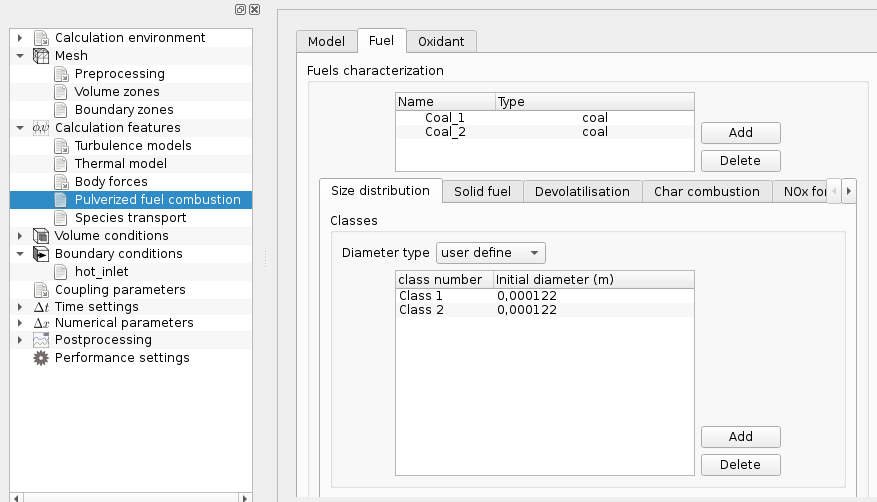
\includegraphics[width=12cm]{gui_coal_classes}
\caption{Thermophysical models - Pulverized coal combustion, coal classes}
\label{fig:Ini-coal1}
\end{center}
\end{figure}

\begin{figure}[!ht]
\begin{center}
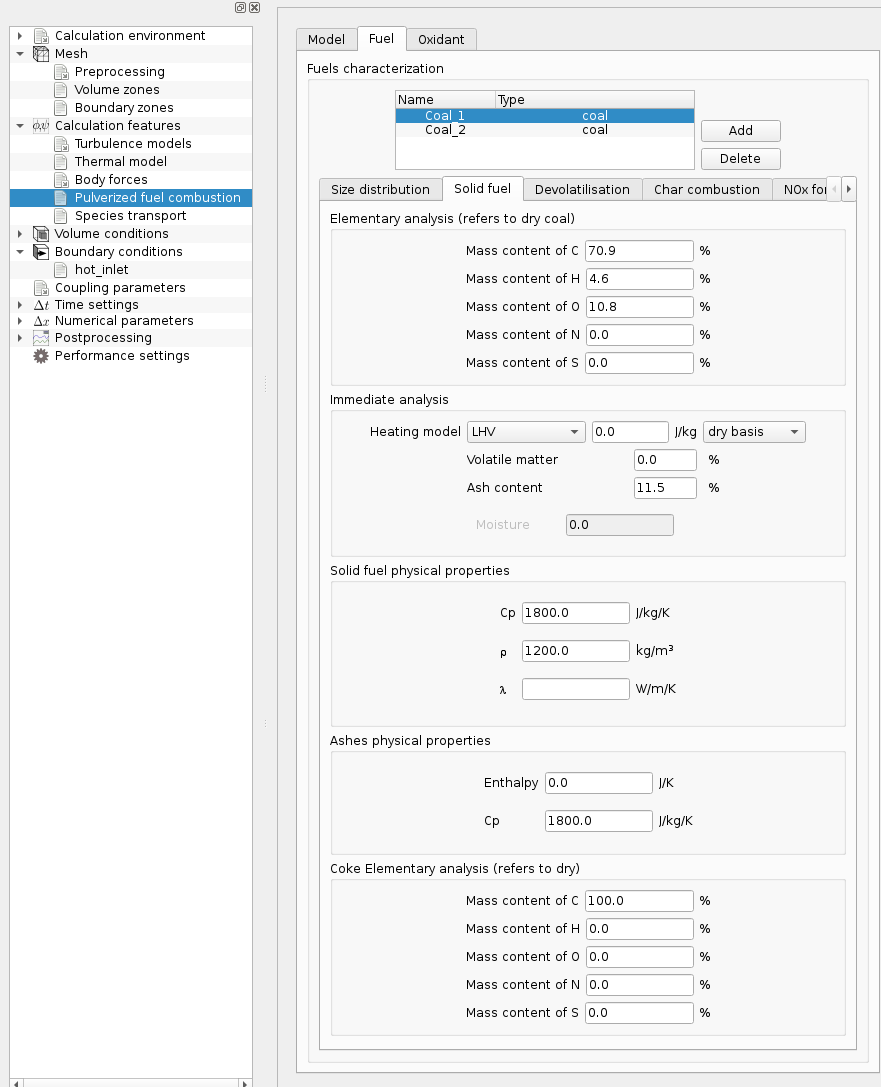
\includegraphics[width=11cm]{gui_coal_composition}
\caption{Pulverized coal combustion, coal composition}
\label{fig:Ini-coal3}
\end{center}
\end{figure}

\begin{figure}[!ht]
\begin{center}
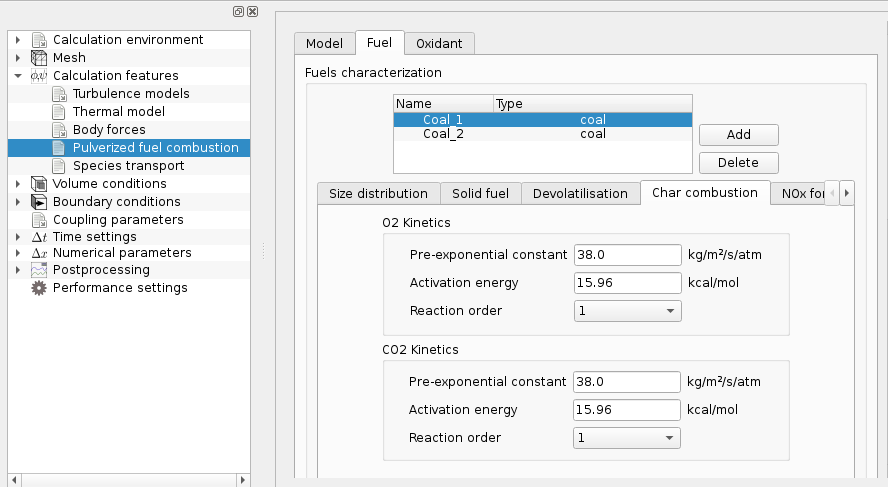
\includegraphics[width=11cm]{gui_coal_reaction}
\caption{Pulverized coal combustion, reaction parameters}
\label{fig:Ini-coal4}
\end{center}
\end{figure}

\begin{figure}[!ht]
\begin{center}
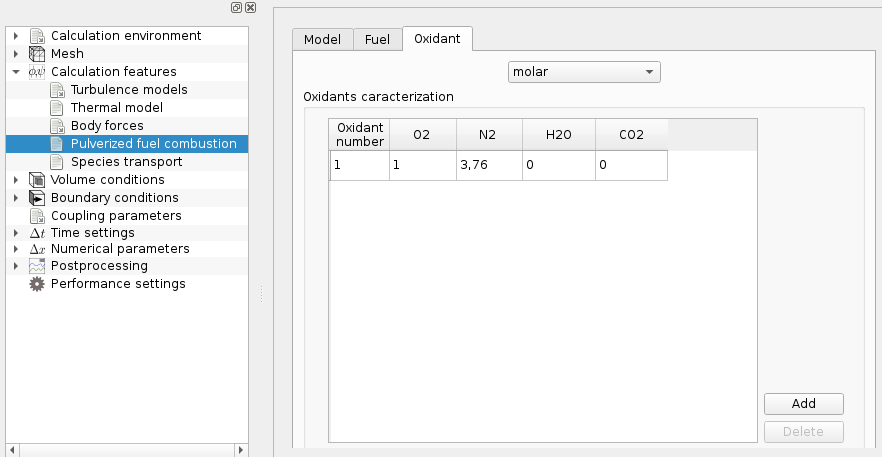
\includegraphics[width=11cm]{gui_coal_oxydant}
\caption{Pulverized coal combustion, oxydant}
\label{fig:Ini-coal5}
\end{center}
\end{figure}

If the user deals with gas combustion or if he (or she) does not want to use the
GUI for coal combustion, the subroutine \texttt{cs\_user\_initialization} must be used (only during the calculation initialisation).\\
In this section, ``specific physics'' will refer to gas combustion or
to pulverised coal combustion.

These subroutines allow the user to initialise some variables specific
to the specific physics activated {\em via} \texttt{usppmo}. As usual,
the user may have access to several geometric variables to discriminate
between different initialisation zones if needed.

It should be recalled again that the user can access the array of values of the
variables as described in the \doxygenfile{field.html}{the \texttt{doxygen}
documentation dedicated to the fields management}. In the following description,
only variables indices \texttt{ivar} are given, but field indices can be
retrieved easily by using \texttt{ivarfl(ivar)}.

{\em WARNING: in the case of a specific physics modelling, all the
variables will be initialised here, even the potential user scalars: {\em
\texttt{cs\_user\_initialization}} is no longer used.}


\begin{list}{$\bullet$}{}
       \item in the case of the EBU pre-mixed flame module, the user can
             initialise in every cell \texttt{iel}: the mixing rate
             \texttt{isca(ifm)} in variable richness, the
             fresh gas mass fraction \\
             \texttt{isca(iygfm\index{iygfm})}
             and the mixture enthalpy \texttt{isca(iscalt)} in
             permeatic conditions

        \item in the case of the rapid complete chemistry diffusion flame
             module, the user can initialise in every cell \texttt{iel}: the
             mixing rate \texttt{isca(ifm\index{ifm})}, its variance
             \texttt{isca(ifp2m\index{ifp2m})} and the mixture mass
             enthalpy \texttt{isca(iscalt)} in permeatic conditions

        \item in the case of the pulverised coal combustion module, the
             user can initialise in every cell \texttt{iel}:
              \begin{list}{$\rightarrow$}{}
                     \item the transport variables related to the solid phase
                           \begin{list}{}{}
                                  \item \texttt{isca(ixch\index{ixch}(icla))}
                                  the reactive coal mass fraction related to the
                                  class \texttt{icla} (\texttt{icla} from 1 to
                                  \texttt{nclacp} which is the total number of
                                  classes, {\em i.e.} for all the coal type)
                                  \item \texttt{isca(ixck(\index{ixck}icla))}
                                  the coke mass fraction related to the class
                                  \texttt{icla}
                                  \item \texttt{isca(inp\index{inp}(icla))} the
                                  number of particles related to class
                                  \texttt{icla} per kg of air-coal mixture
                                  \item \texttt{isca(ih2\index{ih2}(icla))} the
                                   mass enthalpy related to the class
                                   \texttt{icla} in permeatic conditions
                           \end{list}
                     \item \texttt{isca(iscalt)} the mixture enthalpy
                     \item the transport variables related to the gas phase
                           \begin{list}{}{}
                                  \item
                                       \texttt{isca(if1m\index{if1m}(icha))} the
                                       mean value of the tracer 1 representing
                                       the light volatile matters released by
                                       the coal \texttt{icha}
                                  \item
                                       \texttt{isca(if2m\index{if2m}(icha))} the
                                        mean value of the tracer 2 representing
                                        the heavy volatile matters released by
                                        the coal \texttt{icha}
                                  \item \texttt{isca(if3m\index{if3m})}
                                        the mean value of the tracer 3
                                        representing the carbon released
                                        as CO during coke burnout
                                  \item \texttt{isca(if4p2m\index{if4p2m})} the
                                  variance associated with the tracer 4
                                  representing the air (the mean value of this
                                  tracer is not transported, it can be deduced
                                  directly from the three others)
                                  \item \texttt{isca(ifp3m\index{ifp3m})} the
                                  variance associated with the tracer 3
                           \end{list}
              \end{list}
\end{list}

%==================================
\subsubsection{Boundary conditions}\label{sec:coal-cl}
%==================================
In this section, ``specific physics'' refers to gas combustion or
to pulverised coal combustion.\\
For coal combustion, it is possible to manage the boundary conditions in the Graphical User Interface (GUI). When the coal combustion physics is selected in the heading ``Thermophysical models'', specific boundary conditions are activated for inlets, see \figurename~\ref{fig:cond_lim-coal}. The user fills for each type of coal previously defined (see \S~\ref{sec:Ini-coal}) the initial temperature and initial composition of the inlet flow, as well as the mass flow rate.

\begin{figure}[!ht]
\begin{center}
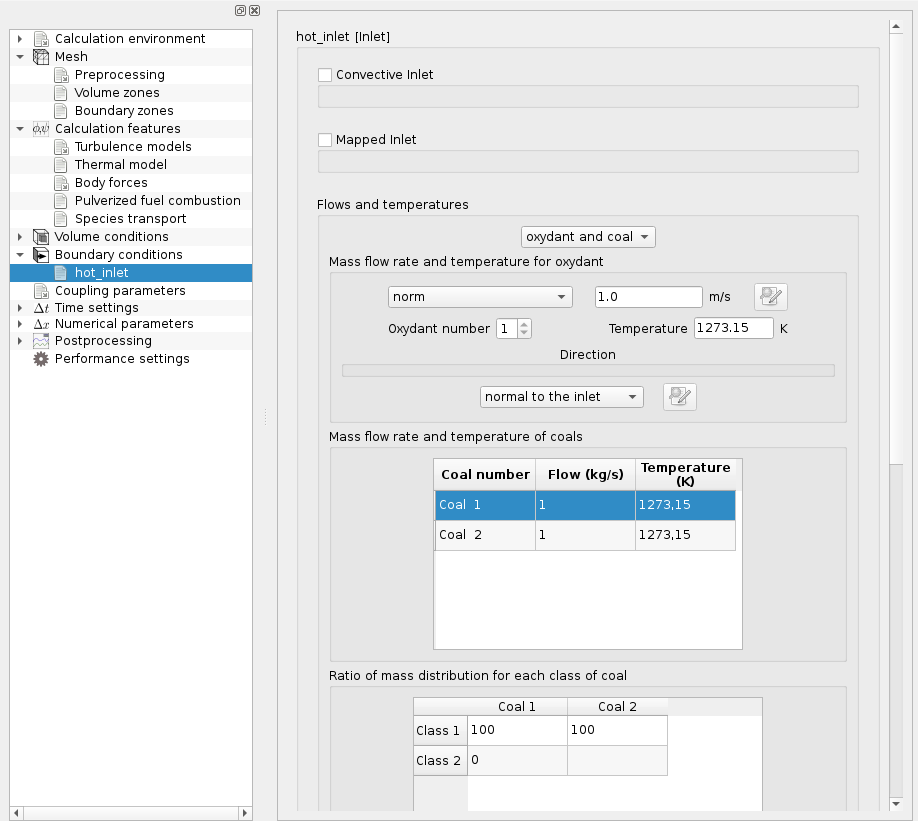
\includegraphics[width=13cm]{gui_coal_bc}
\caption{Boundary conditions for the combustion of coal}
\label{fig:cond_lim-coal}
\end{center}
\end{figure}

For gas combustion or if the GUI is not used for coal combustion, the use of
\texttt{cs\_user\_boundary\_conditions} (called at every time step) is as
mandatory as \texttt{cs\_user\_parameters.f90} and \texttt{usppmo} to run a calculation involving specific physics. The way of using them is the same as using
 in the framework of standard calculations, that is, run several loops on the boundary faces lists (cf. \S\ref{sec:fvm_selector})
marked out by their colors, groups, or  geometrical criterion, where
the type of face, the type of boundary condition for each variable and
eventually the value of each variable are defined.

{\em WARNING: In the case of a specific physics modelling, all the
boundary conditions for every variable must be defined here, even for
the eventual user scalars: {\em \texttt{cs\_user\_boundary\_conditions}} is not used at all.}\\

In the case of a specific physics modelling, a zone number \texttt{izone}
\footnote{\texttt{izone} must be less than the maximum number of boundary
zone allowable by the code, \texttt{nozppm}. This is fixed at 2000 in
 \texttt{pppvar};not to be modified} (for
instance the color \texttt{icoul}) is associated with every boundary face, in
order to gather together all the boundary faces of the same type. In
comparison to \texttt{cs\_user\_boundary\_conditions}, the main change from the user point of
view concerns the faces whose boundary conditions belong to the type
\texttt{itypfb=ientre\index{ientre}}:

\begin{list}{$\bullet$}{}
       \item for the EBU pre-mixed flame module:
             \begin{list}{$\rightarrow$}{}
                    \item the user can choose between the ``burned gas
                          inlet'' type (marked out by the burned gas indicator
                          \texttt{ientgb\index{ientgb}(izone\index{izone})}=1) and the
                          ``fresh gas inlet'' type (marked out by
                          the fresh gas indicator
                          \texttt{ientgf\index{ientgf}(izone)}=1)
                    \item for each inlet type (fresh or burned
                          gas), a mass flow or a velocity must be imposed:

                          \begin{list}{-}{}
                                 \item to impose the mass flow,
                                     \begin{list}{-}{}
                                       \item the user gives to
                                             the indicator
                                             \texttt{iqimp\index{iqimp}(izone)}
                                             the value 1,
                                       \item  the
                                             mass flow value is set in
                                             \texttt{qimp\index{qimp}(izone)}
                                             (positive value, in $kgs^{-1}$)
                                       \item finally he imposes the
                                             velocity vector direction
                                             by giving the components of
                                             a direction vector in
                                             \texttt{rcodcl\index{rcodcl}(ifac,iu\index{iu})}, \texttt{rcodcl(ifac,iv\index{iv})} and \texttt{rcodcl(ifac,iw\index{iw})}
                                     \end{list}

{\em WARNING:
\begin{list}{-}{}
\item the variable \texttt{qimp(izone)} refers to the mass flow across the whole
      zone \texttt{izone} and not across a boundary face (specifically for the axi-symmetric calculations, the inlet surface of the mesh must be broken up)
\item the variable \texttt{qimp(izone)} deals with the inflow across the area \texttt{izoz} and only across this zone; it is recommended to pay attention to the boundary conditions.
\item the velocity direction vector is neither necessarily normed, nor
      necessarily incoming.
\end{list}}

                                 \item to impose a velocity, the user
                                       must give to the indicator
                                       \texttt{iqimp(izone)} the value 0 and set
                                       the three velocity components (in
                                       $m.s^{-1}$) in
                                       \texttt{rcodcl(ifac,iu)},
                                       \texttt{rcodcl(ifac,iv)} and
                                       \texttt{rcodcl(ifac,iw)}
                          \end{list}
                    \item finally he specifies for each gas inlet type
                          the mixing rate \texttt{fment\index{fment}(izone)} and
                          the temperature \texttt{tkent\index{tkent}(izone)} in Kelvin
             \end{list}

       \item for the ``3 points'' diffusion flame module:
             \begin{list}{$\rightarrow$}{}
                    \item the user can choose between the ``oxidiser
                          inlet'' type marked out by
                          \texttt{ientox\index{ientox}(izone)}=1 and the ``fuel
                          inlet'' type marked out by
                          \texttt{ientfu\index{ientfu}(izone)}=1
                    \item concerning the input mass flow or the input
                          velocity, the method is the same as for the
                          EBU pre-mixed flame module
                    \item finally, the user sets the temperatures
                          \texttt{tinoxy\index{tinoxy}} for each oxidiser inlet
                          and \texttt{tinfue\index{tinfue}}, for each fuel inlet

{\em Note: In the standard version, only the cases with only one
                          oxidising inlet type and one fuel inlet type
                          can be treated. In particular, there must be
                          only one input temperature for the oxidiser
                          (\texttt{tinoxy}) and one input temperature for the
                          fuel (\texttt{tinfuel}).}
             \end{list}

       \item for the pulverised coal module:
             \begin{list}{$\rightarrow$}{}
                    \item the inlet faces can belong to the ``primary
                          air and pulverised coal inlet'' type, marked
                          out by \texttt{ientcp\index{ientcp}(izone)}=1, or to
                          the ``secondary or tertiary air inlet'' type,
                          marked out by \texttt{ientat\index{ientat}(izone)}=1
                    \item in a way which is similar to the process
                          described in the framework of the EBU module,
                          the user chooses for every inlet face to
                          impose the mass flow or not (\texttt{iqimp(izone)}=1 or
                          0). If the mass flow is imposed, the user
                          must set the air mass flow value
                          \texttt{qimpat\index{qimpat}(izone)}, its direction in
                          \texttt{rcodcl(ifac,iu)}, \texttt{rcodcl(ifac,iv)}
                          and \\ \texttt{rcodcl(ifac,iw)} and if
                    \item incoming air temperature \texttt{timpat\index{timpat}(izone)} in
                          Kelvin. If the velocity is imposed, he must
                          set  \texttt{rcodcl(ifac,iu)}, \\
                          \texttt{rcodcl(ifac,iv)} and \texttt{rcodcl(ifac,iw)}.

                    \item if the inlet belongs to the ``primary air and
                          pluverised coal'' \texttt{type (ientcp(izone) = 1)} the
                          user must also define for each coal type \texttt{icha}:
                          the mass flow
                          \texttt{qimpcp\index{qimpcp}(izone,icha)}, the
                          granulometric distribution
                          \texttt{distch\index{distch}(izone,icha,iclapc)}
                          related to each class \texttt{iclacp}, and the
                          injection temperature
                          \texttt{timpcp\index{timpcp}(izone,icha)}

             \end{list}
\end{list}

%==================================
\subsubsection{Initialisation of the options of the variables}
%==================================
In the case of coal combustion, time averages, chronological records and logss follow-ups can be set in the Graphical User Interface (GUI) or in the subroutines \texttt{cs\_user\_combustion}. In the GUI, under the heading ``Calculation control'', additional variables appear in the list in the items ``Time averages'' and ``Profiles'', as well as in the item Volume solution control'', see \figurename~\ref{fig:t_average-coal} and \figurename~\ref{fig:V_control-coal}.

\begin{figure}[!ht]
\begin{center}
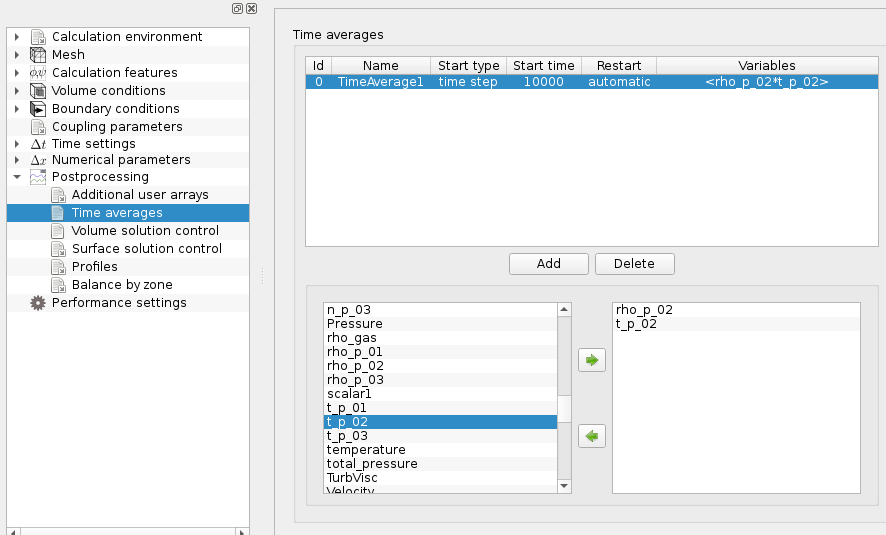
\includegraphics[width=12cm]{gui_coal_time_average}
\caption{Calculation control - Time averages}
\label{fig:t_average-coal}
\end{center}
\end{figure}

\begin{figure}[!ht]
\begin{center}
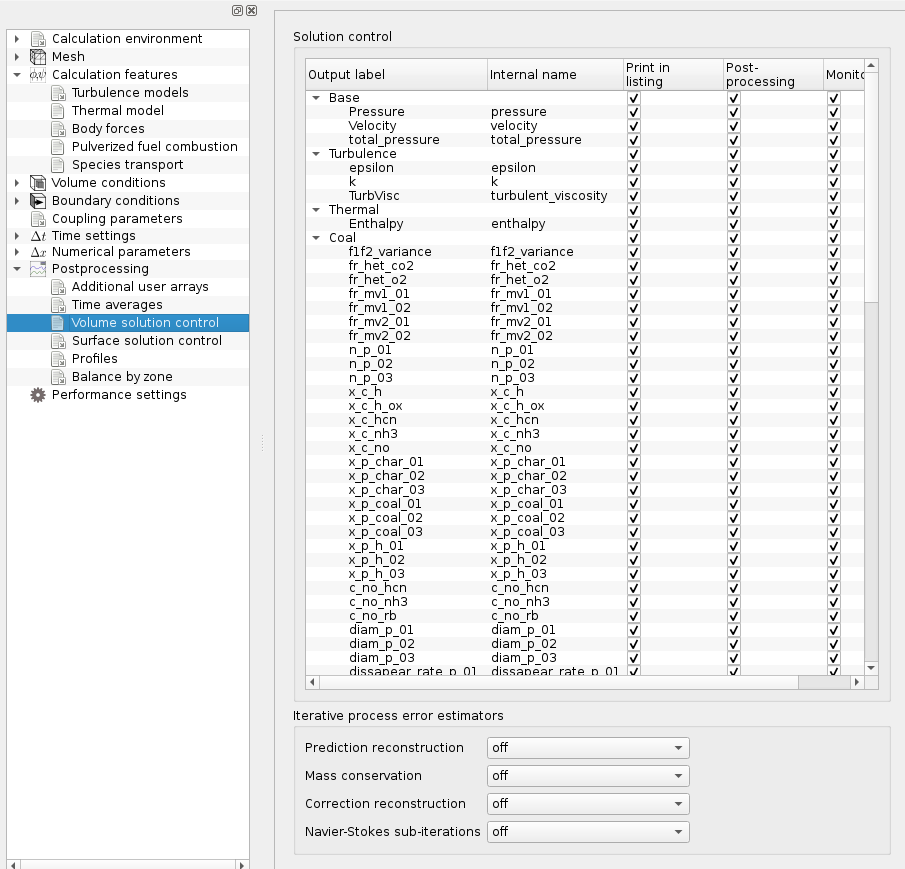
\includegraphics[width=13cm]{gui_coal_solution_control}
\caption{Calculation control - Volume solution control}
\label{fig:V_control-coal}
\end{center}
\end{figure}

In this section, ``specific physics'' refers to gas combustion or
pulverised coal combustion.

For gas combustion or if the GUI is not used for coal combustion, the 3
subroutines \texttt{cs\_user\_combustion} can be used to complete
\texttt{cs\_user\_parameters.f90} for the considered specific physics. These
subroutines are called at the calculation start.
They allow to:
\begin{list}{$\bullet$}{}
\item activate, for the variables which are specific to the activated specific
      physics module, chronological records at the probes defined in
      \texttt{cs\_user\_parameters.f90}.\\
      Concerning the main variables (velocity, pressure, etc ...) the user
      must still complete \texttt{cs\_user\_parameters.f90} if he wants to get
      chronological records, printings in the log or chronological
      outputs.
      The variables which can be activated by the user for each specific
      physics are listed below. The solved variables (of variable indices
      \texttt{ivar}) and the properties of indices \texttt{iprop} (defined at
      the cell \texttt{iel} by \texttt{cpro\_prop(iel)} which is obtained
      by calling \texttt{field\_get\_val\_s(iprop, cpro\_prop)})
      are listed below:
      \begin{list}{$\rightarrow$}{}
       \item EBU pre-mixed flame modelling:
       \begin{list}{-}{}
        \item Solved variables
              \begin{list}{\texttt{ivar} = }{}
               \item \texttt{isca(iygfm\index{iygfm})} fresh gas mass fraction
               \item \texttt{isca(ifm\index{ifm})} mixing rate
               \item \texttt{isca(ihm\index{ihm})} enthalpy, if transported
              \end{list}
        \item Properties \texttt{cpro\_prop(iel)}
              \begin{list}{\texttt{iprop} = }{}
               \item \texttt{itemp\index{itemp}} temperature
               \item \texttt{iym(1)\index{iym(1)}} fuel mass fraction
               \item \texttt{iym(2)\index{iym(2)}} oxidiser mass fraction
               \item \texttt{iym(3)\index{iym(3)}} product mass fraction
               \item \texttt{ickabs\index{ickabs}} absorption
                     coefficient, when the radiation modelling is
                     activated
               \item \texttt{it3m\index{it3m}} and \texttt{it4m\index{it4m}}
                     ``$T^3$'' and ``$T^4$'' terms, when the radiation
                     modelling is activated
              \end{list}
       \end{list}
       \item rapid complete chemistry diffusion flame modelling:
             \begin{list}{}{}
              \item  everything is identical to the ``EBU'' case, except
                     the fresh gas mass fraction which is replaced by the
                     variance of the mixing rate
                     \texttt{ivar=isca(ifp2m\index{ifp2m})}
             \end{list}
       \item pulverised coal modelling with 3 combustibles:
             \begin{list}{}{}
              \item {\em variables shared by the two phases}:
                    \begin{list}{-}{}
                     \item Solved variables
                           \begin{list}{\texttt{ivar} = }{}
                            \item \texttt{isca(ihm\index{ihm})}: gas-coal
                                  mixture enthalpy
                            \item \texttt{isca(immel\index{immel})}: molar mass
                                  of the gas mixture
                           \end{list}
                    \end{list}
              \item {\em variables specific to the dispersed phase}:
              \begin{list}{-}{}
               \item Solved variables
                     \begin{list}{\texttt{ivar} = }{}
                      \item \texttt{isca(ixck\index{ixck}(icla))}: coke mass
                            fraction related to the class \texttt{icla}
                      \item \texttt{isca(ixch\index{ixch}(icla))}: reactive coal
                            mass fraction related to the class \texttt{icla}
                      \item \texttt{isca(inp\index{inp}(icla))}: number of
                            particles of the class \texttt{icla} per kg of
                            air-coal mixture
                      \item \texttt{isca(ih2\index{ih2}(icla))}: mass enthalpy
                            of the coal of class \texttt{icla}, if we are in
                            permeatic conditions
                     \end{list}
               \item Properties \texttt{cpro\_prop(iel)}
                     \begin{list}{\texttt{iprop} = }{}
                      \item \texttt{immel\index{immel}}: molar mass of the gas
                            mixture
                      \item \texttt{itemp2\index{itemp2}(icla)}: temperature of
                            the particles of the class \texttt{icla}
                      \item \texttt{irom2\index{irom2}(icla)}: density of
                            the particles of the class \texttt{icla}
                      \item \texttt{idiam2\index{idiam2}(icla)}: diameter of the
                            particles of the class \texttt{icla}
                      \item \texttt{igmdch\index{igmdch}(icla)}: disappearance
                            rate of the reactive coal of the class \texttt{icla}
                      \item \texttt{igmdv1\index{igmdv1}(icla)}: mass transfer
                            caused by the release of light volatiles
                            from the class \texttt{icla}
                      \item \texttt{igmdv2\index{igmdv2}(icla)}: mass transfer
                            caused by the release of heavy volatiles
                            from the class \texttt{icla}
                      \item \texttt{igmhet\index{igmhet}(icla)}: coke
                            disappearance rate during the coke burnout
                            of the class \texttt{icla}
                      \item \texttt{ix2\index{ix2}(icla)}: solid mass fraction
                            of the class \texttt{icla}
                     \end{list}
              \end{list}
              \item {\em variables specific to the continuous phase}:
              \begin{list}{-}{}
               \item Solved variables
                     \begin{list}{\texttt{ivar} = }{}
                      \item \texttt{isca(if1m\index{if1m}(icha))}: mean value of
                            the tracer 1 representing the light
                            volatiles released by the coal \texttt{icha}
                      \item \texttt{isca(if2m\index{if2m}(icha))}: mean value of
                            the tracer 2 representing the heavy
                            volatiles released by the coal \texttt{icha}
                      \item \texttt{isca(if3m)\index{if3m}}: mean value of the
                            tracer 3 representing the carbon released as
                            CO during coke burnout
                      \item \texttt{isca(if4pm\index{if4pm})}: variance of the
                            tracer 4 representing the air
                      \item \texttt{isca(if3p2m\index{if3p2m})}: variance of the
                            tracer 3
                     \end{list}
               \item Properties \texttt{cpro\_prop(iel)}
                     \begin{list}{\texttt{iprop} = }{}
                      \item \texttt{itemp\index{itemp1}}: temperature of the
                            gas mixture
                      \item \texttt{iym1(1)\index{iym1(1)}}: mass fraction of
                            $CH_{X1m}$ (light volatiles) in the gas
                            mixture
                      \item \texttt{iym1(2)\index{iym1(2)}}: mass fraction of
                            $CH_{X2m}$ (heavy volatiles) in the gas
                            mixture
                      \item \texttt{iym1(3)\index{iym1(3)}}: mass fraction of
                            CO in the gas mixture
                      \item \texttt{iym1(4)\index{iym1(4)}}: mass fraction of
                            $O_2$ in the gas mixture
                      \item \texttt{iym1(5)\index{iym1(5)}}: mass fraction of
                            $CO_2$ in the gas mixture
                      \item \texttt{iym1(6)\index{iym1(6)}}: mass fraction of
                            $H_2O$ in the gas mixture
                      \item \texttt{iym1(7)\index{iym1(7)}}: mass fraction of
                            $N_2$ in the gas mixture
                     \end{list}
              \end{list}
             \end{list}
      \end{list}

 \item set the relaxation coefficient of the density \texttt{srrom}, with \\
$\rho^{n+1}=\texttt{srrom}*\rho^{n}+(1-\texttt{srrom})\rho^{n+1}$\\
(the default value is \texttt{srrom\index{srrom}} = 0.8. At the
      beginning of a calculation, a sub-relaxation of 0.95 may reduce
      the numerical ``shocks'').

 \item set the dynamic viscosity \texttt{diftl0}. By default
      \texttt{diftl0\index{diftl0}}= 4.25 $kgm^{-1}s^{-1}$
(the dynamic diffusivity being the ratio between the thermal
      conductivity $\lambda$ and the mixture specific heat $C_p$ in the
      equation of enthalpy).

 \item set the value of the constant \texttt{cebu\index{cebu}} of the Eddy Break
      Up model (only in \texttt{cs\_user\_combustion}. By default \texttt{cebu}=2.5)
\end{list}

%==================================
\subsection{Heavy fuel oil combustion module}
%==================================
%==================================
\subsubsection{Initialisation of transported variables}
%==================================
To initialise or modify (in case of a continuation) values of transported
variables and of the time step, the standard subroutine \texttt{cs\_user\_initialization} is used.

Physical properties are stored using the \texttt{cs\_field} API (cell center). For instance, to obtain \texttt{rom(iel)},
the mean density (in $kg.m^{-3}$), one must declare a \texttt{ncelet} array \texttt{cpro\_rom} and then call
\texttt{call field\_get\_val\_s(icrom, cpro\_rom)}.\\
Physical properties (\texttt{rom, viscl, cp, ...}) are computed in \texttt{ppphyv} and are not to be modified here.

The \texttt{cs\_user\_initialization-fuel.f90} example illustrates how the user
may initialise quantities related to gaseous species and droplets compositions
in addition to the chosen turbulent model.

%==================================
\subsubsection{Boundary conditions}
%==================================
Boundary conditions are defined as usual on a per-face basis in
\texttt{cs\_user\_boundary\_conditions}. They may be assigned in two ways:
\begin{list}{.}{}
\item for ``standard'' boundary conditions (inlet, free outlet, wall, symmetry): a code is defined in the array \texttt{itypfb} (of dimensions equal to the number of boundary faces). This code will then be used by a non-user subroutine to assign the conditions.
\item for ``non-standard'' conditions: see details given in
  \texttt{cs\_user\_boundary\_conditions-fuel.f90} example.
\end{list}

%==================================
\subsection{Radiative thermal transfers in semi-transparent gray media}
%==================================
%==================================
\subsubsection{Initialisation of the radiation main parameters}
%==================================

The main radiation parameters can be initialise in the Graphical User Interface (GUI) or in the user subroutine \texttt{cs\_user\_radiative\_transfer\_param}. In the GUI, under the heading ``Thermophysical models'', when one of the two thermal radiative transfers models is selected, see \figurename~\ref{fig:0_ray}, additional items appear. The user is asked to choose the number of directions for angular discretisation, to define the absorption coefficient and select if the radiative calculation are restarted or not,
see \figurename~\ref{fig:1_ray} and \figurename~\ref{fig:3_ray}. When ``Advanced options'' is selected for both models \figurename~\ref{fig:2_ray} or \figurename~\ref{fig:4_ray} appear, the user must fill the resolution frequency and verbosity levels. In addition, the activation of the radiative transfer leads to the creation of an item ``Surface solution control'' under the heading ``Calculation control'',
see \figurename~\ref{fig:5_ray}, where radiative transfer variables can be selected to appear in the output log.

\begin{figure}[ht]
\begin{center}
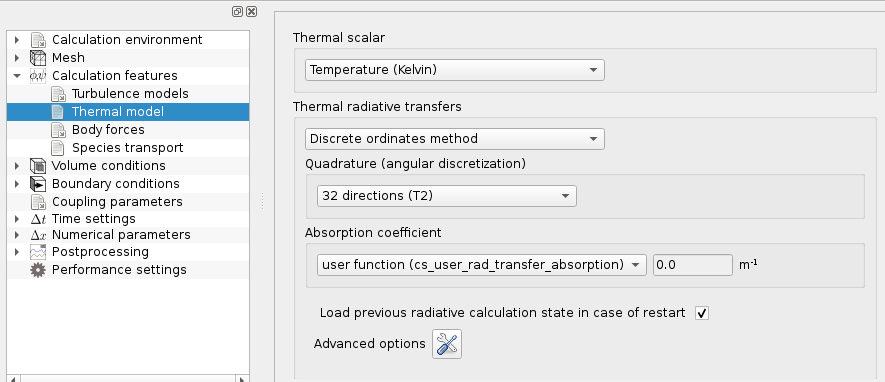
\includegraphics[width=0.9\textwidth]{gui_rad_transf_do_params}
\caption{Radiative transfers - parameters of the DO method}
\label{fig:1_ray}
\end{center}
\end{figure}

\begin{figure}[ht]
\begin{center}
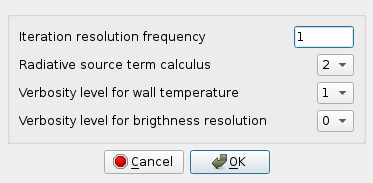
\includegraphics[width=7cm]{gui_rad_transf_do_advanced}
\caption{Radiative transfers - advanced parameters of the DO method}
\label{fig:2_ray}
\end{center}
\end{figure}

\begin{figure}[ht]
\begin{center}
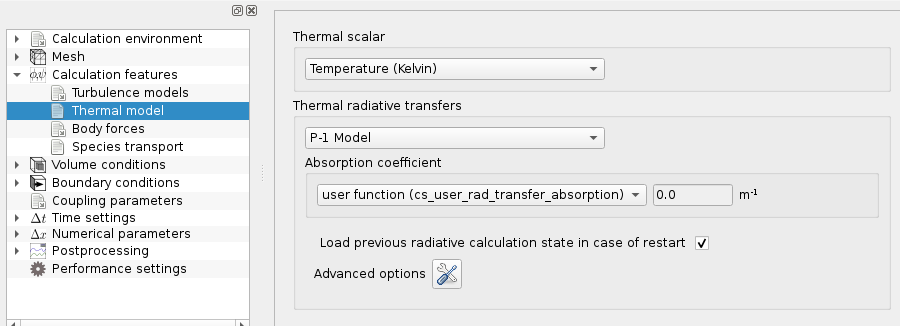
\includegraphics[width=0.9\textwidth]{gui_rad_transf_p1_params}
\caption{Radiative transfers - parameters of the P-1 model}
\label{fig:3_ray}
\end{center}
\end{figure}

\begin{figure}[ht]
\begin{center}
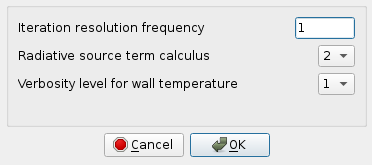
\includegraphics[width=7cm]{gui_rad_transf_p1_advanced}
\caption{Radiative transfers - advanced parameters of the P-1 model}
\label{fig:4_ray}
\end{center}
\end{figure}

\begin{figure}[ht]
\begin{center}
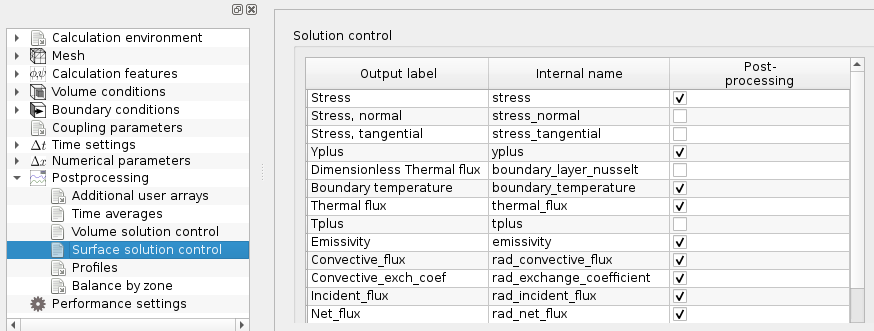
\includegraphics[width=0.9\textwidth]{gui_rad_transf_post_output}
\caption{Calculation control - Radiative transfers post-processing output}
\label{fig:5_ray}
\end{center}
\end{figure}

If the GUI is not used, \texttt{cs\_user\_radiative\_transfer\_param} is one of the two subroutine which must be completed by the user for all
calculations including radiative thermal transfers. It is called only during the calculation initialisation. It is composed of three headings. The first one is dedicated to the activation
of the radiation module, only in the case of classic physics. \\
{\em WARNING: when a calculation is ran using a specific physics module,
this first heading must not be completed. The radiation module is then
activated or not, according to the parameter file related to the considered
specific physics.} \\

\noindent
In the second heading the basic parameters of the radiation module are indicated.\\
Finally, the third heading deals with the selection of the
post-processing graphic outputs. The variables to treat are splitted
into two categories: the volumetric variables and those related to the
boundary faces.\\

\noindent
For more details about the different parameters, the user may refer to the
keyword list (\S~\ref{sec:prg_motscles}).


%==================================
\subsubsection{Radiative transfers boundary conditions}
%==================================
These informations can be filled by the user through the Graphical User Interface
(GUI) or by using the subroutine \texttt{cs\_user\_radiative\_transfer\_bcs.c} (called every time step). If the
interface is used, when one of the ``Radiative transfers'' options is selected in
\figurename~\ref{fig:gui_thermal_scalar}, it activates specific boundary conditions each time
a ``Wall'' is defined, see \figurename~\ref{fig:6_ray}. The user can then choose
between 3 cases. The parameters the user must specify are displayed for one of
them in \figurename~\ref{fig:7_ray}.

\begin{figure}[ht]
\begin{center}
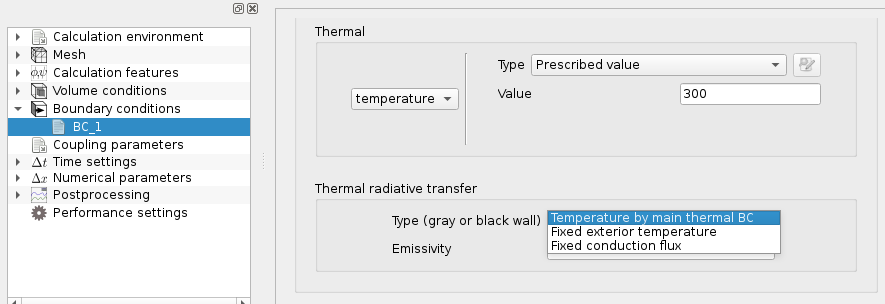
\includegraphics[width=0.9\textwidth]{gui_rad_transf_wall_model}
\caption{Boundary conditions - choice of wall thermal radiative transfers}
\label{fig:6_ray}
\end{center}
\end{figure}

\begin{figure}[ht]
\begin{center}
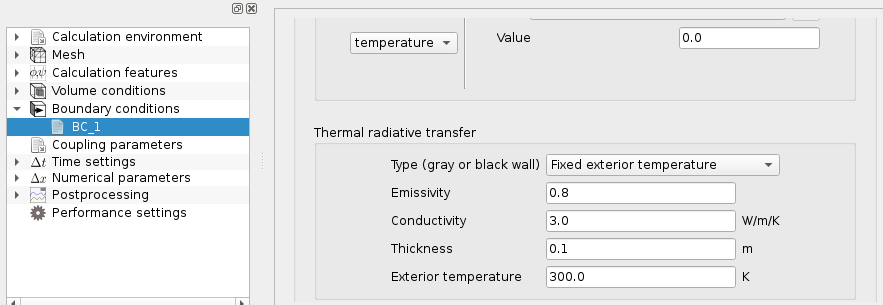
\includegraphics[width=0.9\textwidth]{gui_rad_transf_wall_params}
\caption{Boundary conditions - example of wall thermal radiative transfer}
\label{fig:7_ray}
\end{center}
\end{figure}

When the GUI is not used, \texttt{cs\_user\_radiative\_transfer\_bcs.c} is needed for
every calculation which includes radiative thermal transfers. It is used to give all the
necessary parameters concerning, in the one case, the wall temperature
calculation, and in the other, the coupling between the thermal
scalar (temperature or enthalpy), and the radiation module at the
calculation domain boundaries. It must be noted that the boundary conditions
concerning the thermal scalar which may have been defined in the
GUI or in subroutine \texttt{cs\_user\_boundary\_conditions} will be modified by
the radiation module according to the data given in \texttt{cs\_user\_radiative\_transfer\_bcs} (cf. \S\ref{sec:fvm_selector}).\\
A boundary condition type stored in the array \texttt{isothp} is associated with
each boundary face. There are five different types:

\begin{list}{$\bullet$}{}

\item \texttt{\textbf{CS\_BOUNDARY\_RAD\_WALL\_GREY}}: grey of black wall, with
      temperature defined by main (fluid) boundary conditions,

\item \texttt{\textbf{CS\_BOUNDARY\_RAD\_WALL\_GREY\_EXTERIOR\_T}}:
       grey or black wall, calculation of the temperature by means of a flux balance
       with an exterior temperature,

\item \texttt{\textbf{CS\_BOUNDARY\_RAD\_WALL\_REFL\_EXTERIOR\_T}}:
      for a reflecting wall face, calculation of the
      temperature by means of a flux balance. This is equivalent to
      using \textbf{CS\_BOUNDARY\_RAD\_WALL\_GRAY\_EXTERIOR\_T},
      with zero emissivity.

\item \texttt{\textbf{CS\_BOUNDARY\_RAD\_WALL\_GRAY\_COND\_FLUX}}:
      grey or black wall face to which a conduction
      flux is imposed,

\item \texttt{\textbf{CS\_BOUNDARY\_RAD\_WALL\_REFL\_COND\_FLUX}}:
      reflecting wall face to which a conduction
      flux is imposed, which is equivalent to impose this flux directly
      to the fluid.

\item \texttt{\textbf{ifinfe}}: for an open boundary (inlet or outlet) or symmetry face,
      simulate an infinite extrusion by applying a Neumann condition to
      the radiation equations,

\end{list}

\noindent
Depending on the selected boundary condition type at every wall face,
the code needs to be given some additional information:

\begin{list}{$\bullet$}{}

\item \texttt{\textbf{CS\_BOUNDARY\_RAD\_WALL\_GRAY}}: the array \texttt{epsp} must
      be completed with the emissivity value (positive).

\item \texttt{\textbf{CS\_BOUNDARY\_RAD\_WALL\_GREY\_EXTERIOR\_T}}: wall emissivity
      (strictly positive, in \texttt{epsp}), thickness (in \texttt{epap}),
      thermal conductivity (in \texttt{xlamp}) and external temperature
      (in \texttt{textp}) in order to calculate a conduction flux across the wall.

\item \texttt{\textbf{CS\_BOUNDARY\_RAD\_WALL\_REFL\_EXTERIOR\_T}}:
      wall thickness (in \texttt{epap}) and thermal
      conductivity (in \texttt{xlamp}) and an external temperature
      (in \texttt{textp}).
      This is equivalent to using \textbf{CS\_BOUNDARY\_RAD\_WALL\_GREY\_EXTERIOR\_T}
      with a wall emissivity of 0, and an exchange coefficient-type boundary
      condition, where the exchange coefficient is equal to
      \texttt{xlamp} / \texttt{textp}.

\item \texttt{\textbf{CS\_BOUNDARY\_RAD\_WALL\_GRAY\_COND\_FLUX}}:
      wall emissivity (in \texttt{epsp}) and conduction
      flux (in $W/m^2$ whatever the thermal scalar, enthalpy or temperature) in
      the array \texttt{rcodcl}. The value of \texttt{rcodcl} is positive when the
      conduction flux is directed from the inside of the fluid domain to the
      outside (for instance, when the fluid heats the walls). If the
      conduction flux is null, the wall is adiabatic.

\item \texttt{\textbf{CS\_BOUNDARY\_RAD\_WALL\_REFL\_COND\_FLUX}}:
      must be given: the conduction flux (in $W/m^2$ whatever the thermal
      scalar) in the array \texttt{rcodcl}. The value of \texttt{rcodcl} is
      positive when the conduction flux is directed from the inside of the
      fluid domain to the outside (for instance, when the fluid heats the
      walls). If the conduction flux is null, the wall is adiabatic. The flux
      received by \texttt{rcodcl} is directly imposed as boundary condition for
      the fluid.

\end{list}

%==================================
\subsubsection{Absorption coefficient of the medium, boundary conditions
   for the luminance and calculation of the net radiative flux}
%==================================

When the absorption coefficient is not constant, the subroutine
\texttt{cs\_user\_rad\_transfer\_absorption} is called instead at each time
step. It is composed of three parts. In the first one, the user
must provide the absorption coefficient of the medium in the array CK,
for each cell of the fluid mesh. By default, the absorption coefficient
of the medium is 0, which corresponds to a transparent medium.\\

{\em WARNING: when a specific physics is activated, it is forbidden to
give a value to the absorption coefficient in this subroutine. In this
case, the coefficient is either calculated automatically, or provided by the user {\em via} a
thermo-chemical parameter file (dp\_C3P or dp\_C3PSJ for gas combustion,
and dp\_FCP for pulverised coal combustion).}\\

\noindent
The two following parts of this subroutine concern a more advanced use
of the radiation module. It is about imposing boundary conditions to the
equation of radiative transfer and net radiative flux calculation, in
coherence with the luminance at the boundary faces, when the user wants
to give it a particular value. In most cases, the given examples do not
need to be modified.

%==================================
\subsection{Conjugate heat transfer}
%==================================

%========================================
\subsubsection{Thermal module in a 1D wall}
%========================================

\noindent
\textit{subroutine called at every time step}

This subroutine takes into account the wall-affected thermal inertia.
 Some boundary faces are treated as a solid wall with a given thickness, on
 which the code resolves a one-dimensional equation for the heat conduction.
 The coupling between the 1D module and the fluid works in a similar way to
 the coupling with the \syrthes. By construction, the user is not able to
 account for the heat transfer between different parts of the wall. A physical
 analysis of each problem, case by case is required in order to evaluate the relevance
 of its usage by way of a report of the simple conditions (temperature, zero-flux
 ) or a coupling with \syrthes.\\

The use of this code requires that the thermal scalar is
defined as (\texttt{iscalt}$>0$).

{\em WARNING: The 1D thermal module is developed assuming the thermal scalar
 as a temperature. If the thermal scalar is an enthalpy, the code calls the
 enthalpy to temperature conversion as defined by the model defaults,
 or by the user in \texttt{cs\_user\_physical\_properties} for each
 transfer of data between the fluid and the wall in order to convert the
 enthalpy to temperature and vice-versa. If the thermal
 variable is the total (compressible) energy, the thermal module will not work.}

%==================================
\subsubsection{Internal Fluid-Thermal coupling}
%==================================

When at least one volume zone is defined as being solid
(see \figurename\ref{fig:internal_coupling_vol_solid}), scalar variables (especially
thermal scalar variables) may be solved in a fully coupled manner across the fluid
and solid domains.

For this purpose, the ``Internal coupling'' should be activated for the desired variables
in the matching tab of the ``Coupling parameters'' page, as shown in figure
\figurename\ref{fig:internal_coupling_param}). This section should appear when
at least one volume zone is defined as solid.

\begin{figure}[ht]
\begin{center}
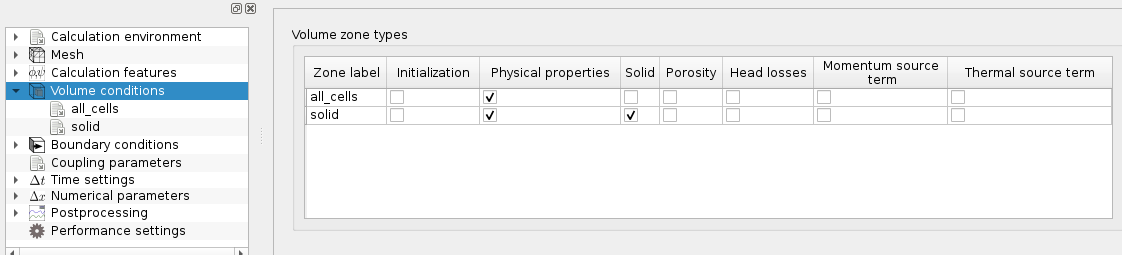
\includegraphics[width=0.9\textwidth]{gui_internal_coupling_vol_zone}
\caption{Solid volume zone definition}
\label{fig:internal_coupling_vol_solid}
\end{center}
\end{figure}

\begin{figure}[ht]
\begin{center}
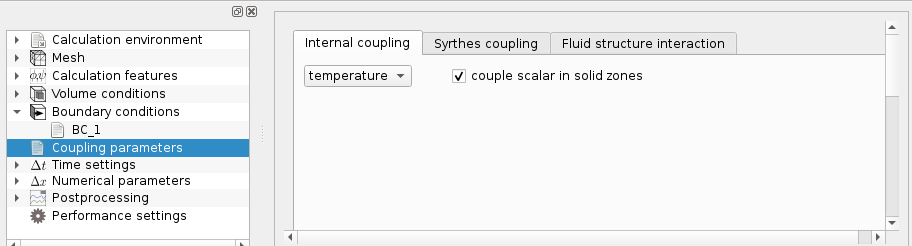
\includegraphics[width=0.9\textwidth]{gui_internal_coupling}
\caption{Conjugate heat transfer: internal coupling}
\label{fig:internal_coupling_param}
\end{center}
\end{figure}

%==================================
\subsubsection{Fluid-Thermal coupling with \syrthes}
%==================================
Coupling \CS with \syrthes for conjugate heat transfer can be defined through
the GUI or the \texttt{cs\_syrthes\_coupling} user function.
To set such a coupling in the GUI, a thermal scalar must be
selected first in the item ``Thermal scalar'' under the heading ``Thermophysical models''.
At least one wall boundary condition must be set to ``SYRTHES coupling'' type, and
the name of the associated \syrthes instance (i.e. base directory name of the associated
solid case definition) be set, as shown in, \figurename\ref{fig:syrthes_bc}.
The ``Syrthes coupling'' tab will then be available in the ``Coupling parameters''
section (see \figurename\ref{fig:syrthes}), fo further advanced or global settings.
The zones where the coupling occurs must be defined and a projection axis can be
specified in case of 2D coupling.

\begin{figure}[ht]
\begin{center}
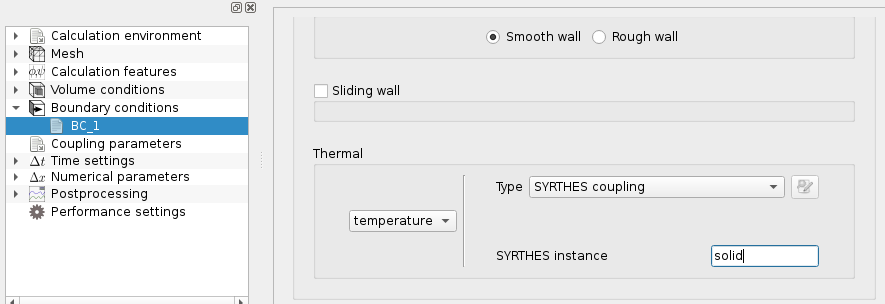
\includegraphics[width=0.9\textwidth]{gui_syrthes_coupling_bc}
\caption{Boundary conditions - coupling with \syrthes}
\label{fig:syrthes_bc}
\end{center}
\end{figure}

\begin{figure}[ht]
\begin{center}
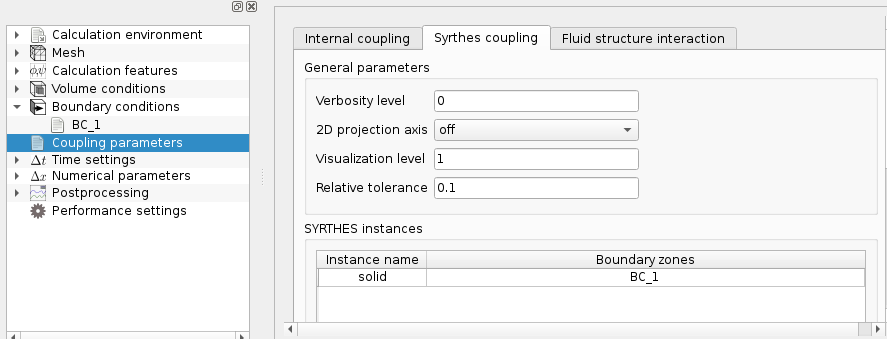
\includegraphics[width=0.9\textwidth]{gui_syrthes_coupling}
\caption{Coupling parameters - coupling with \syrthes}
\label{fig:syrthes}
\end{center}
\end{figure}

If the function \texttt{cs\_user\_syrthes\_coupling} is used, the user must
specify the arguments passed to the '\texttt{cs\_syr\_coupling\_define}' function.
 These arguments are:
\begin{list}{-}{}
 \item \texttt{syrthes\_name} is the matching \syrthes application name (useful only when more than one \syrthes and one \CS domain are present),
 \item \texttt{boundary\_criteria} is the surface selection criteria,
 \item \texttt{volume\_criteria} is the volume selection criteria,
 \item \texttt{projection\_axis}: ' ' if the user wishes to use a 3D standard coupling,
 or specify '$x$', '$y$', or '$z$' as the projection axis if a 2D coupling with \syrthes is used,
 \item \texttt{verbosity} is the verbosity level.
 \item \texttt{visualization} is the visualization level.
\end{list}
Examples are provided in \texttt{cs\_user\_coupling.c}.

The user may also define global coupling options relative to the handling of
time-stepping, by adapting the example \texttt{cs\_user\_coupling}
in the \texttt{cs\_user\_coupling.c} file. In the case of multiple couplings,
these options are global to all \syrthes and \CS couplings.

%==================================
\subsection{Particle-tracking (Lagrangian) Module}
%==================================

%==================================
\subsubsection{General information}\label{sec:over-lag}
%==================================

\begin{itemize}

\item[-] The particle-tracking (or Lagrangian) module enables the simulation of poly-dispersed particulate flows, by calculating the trajectories of individual particles, mainly characterized by their diameter and density (if no heat nor mass transfer between particle and fluid are activated).

\item[-] The standard use of the particle-tracking module follows the \textbf{Moments/PDF approach}: the instantaneous properties of the underlying flow needed to calculate the particle motion are reconstructed from the averaged values (obtained by Reynolds-Averaged Navier-Stokes simulation) by using stochastic processes. The statistics of interest are then obtained through Monte-Carlo simulation.

\item[-] As a consequence, is is important to emphasize that the most important (and physically meaningful) results of a particle-tracking calculation following the Moments/PDF approach are \mbox{\textbf{statistics}}. Volume and surface statistics, steady or unsteady, can be calculated. Individual particle trajectories (as 1D, \textit{EnSight}-readable cases) and displacements (as \textit{EnSight}-readable animations) can also be provided, but only for illustrative purposes.

\end{itemize}

%==================================
\subsubsection{Activating the particle-tracking module}\label{sec:acti-lag}
%==================================

The activation of the particle-tracking module is performed either:
%
\begin{itemize}
 \item [$\bullet$] in the Graphical User Interface (GUI): \texttt{Calculation features} $\rightarrow$ \texttt{Thermophysical models} $\rightarrow$ \texttt{Eulerian-Lagrangian multi-phase treatment}~$\rightarrow$ ~\texttt{particles and droplets tracking}
 \item [$\bullet$] or in the user function \texttt{cs\_user\_lagr\_model}.
\end{itemize}

%==================================
\subsubsection{Basic guidelines for standard simulations}
%==================================

Except for cases in which the flow conditions depend on time, it is generally recommended to perform a first Lagrangian calculation whose aim is to reach a steady-state (i.e. to reach a time starting from which the relevant statistics do not depend on time anymore). In a second step, a calculation restart is done to calculate the statistics. When the single-phase flow is steady and the particle volume fraction is low enough to neglect the particles influence on the continuous phase behaviour, it is recommended to perform a Lagrangian calculation on a frozen field.\\

It is then possible to calculate steady-state volumetric statistics and to give a statistical weight higher than 1 to the particles, in order to reduce the number of simulated (``numerical'') particles to treat while keeping the right concentrations. Otherwise, when the continuous phase flow is steady, but the two-coupling coupling must be taken into consideration, it is still possible to activate steady statistics. \\
When the continuous phase flow is unsteady, it is no longer possible to use steady statistics. To have correct statistics at every moment in the whole calculation domain, it is imperative to have an established particle seeding and it is recommended (when it is possible) not to impose statistical weights different from the unity. \\

Finally, when the so-called complete model is used for turbulent dispersion modelling, the user must make sure that the volumetric statistics are directly used for the calculation of the locally undisturbed fluid flow field.\\

When the thermal evolution of the particles is activated, the associated particulate scalars are always the inclusion temperature and the locally undisturbed fluid flow temperature expressed in degrees Celsius, whatever the thermal scalar associated with the continuous phase is ({\em i.e.} temperature or enthalpy). If the
thermal scalar associated with the continuous phase is the temperature in Kelvin, the unit is converted automatically into Celsius. If the thermal scalar associated with the continuous phase is the enthalpy, a \texttt{temperature} property or postprocessing
field must be defined. In all cases, the thermal backward coupling of the dispersed phase on the continuous phase is adapted to the thermal scalar transported by the fluid.


%==================================
\subsubsection{Prescribing the main modelling parameters}\label{sec:Ini-lag}
%==================================

\minititre{Use of the GUI}

In the GUI, the selection of the Lagrangian module activates the heading \texttt{Particle and droplets tracking} in the tree menu. The initialization is performed in the three items included in this heading:
%
\begin{itemize}
 \item [$\bullet$] \texttt{Global settings}. The user defines in this item the kind of Euler/Lagrange multi-phase treatment, the main parameters, and the specific physics associated with the particles, see ~\figurename~\ref {fig:Ini-Lag1} to \figurename\ref {fig:Ini-Lag3}.
 \item [$\bullet$] \texttt{Statistics}. The user can select the volume and boundary statistics to be post-processed.
 \item [$\bullet$] \texttt{Output}. An additional entry in the postprocessing section allows defining the output frequency and post-processing options for particles and selecting the variables that will appear in the log.
\end{itemize}

\begin{figure}[ht]
\begin{center}
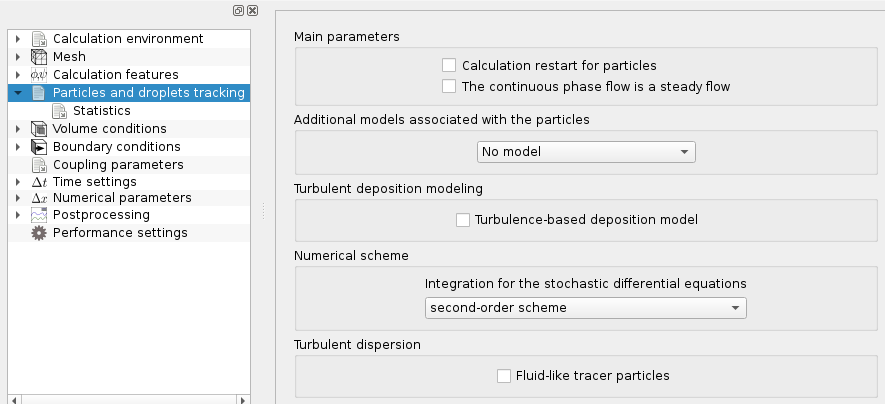
\includegraphics[width=0.9\textwidth]{gui_lagr_global_settings}
\caption{Lagrangian module - View of the \texttt{Global Settings} page}
\label{fig:Ini-Lag1}
\end{center}
\end{figure}

\begin{figure}[ht]
\begin{center}
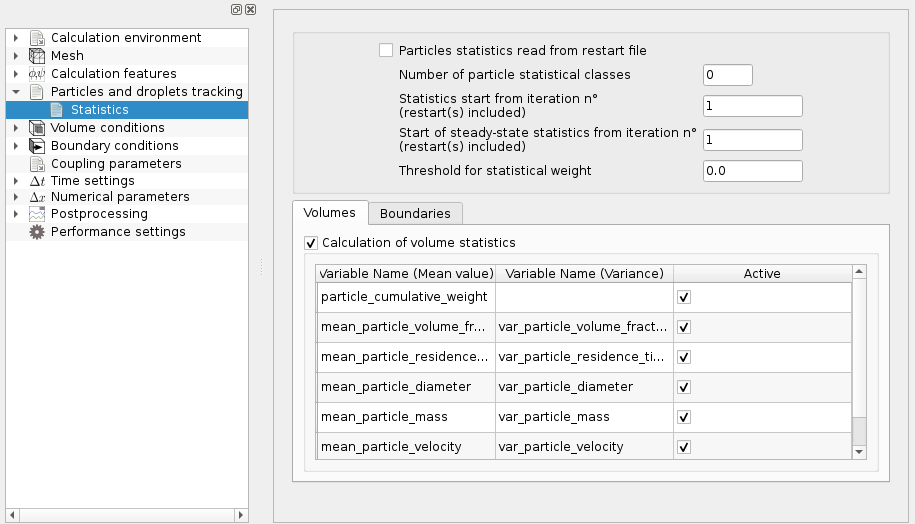
\includegraphics[width=11cm]{gui_lagr_statistics}
\caption{Lagrangian module - statistics}
\label{fig:Ini-Lag4}
\end{center}
\end{figure}

\begin{figure}[ht]
\begin{center}
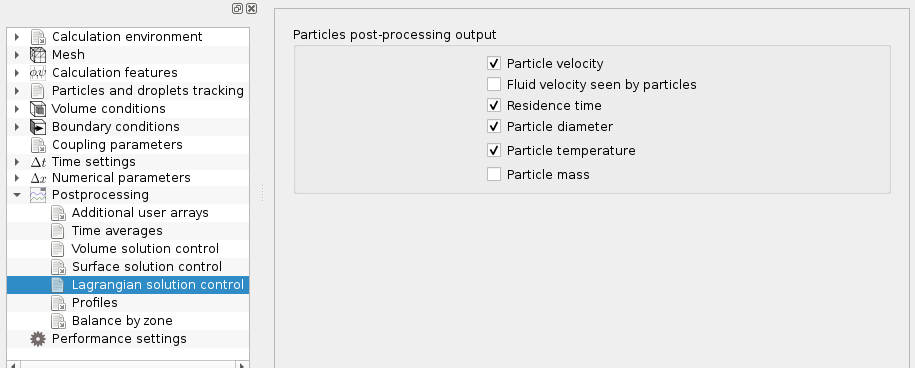
\includegraphics[width=11cm]{gui_lagr_output}
\caption{Lagrangian module - output}
\label{fig:Ini-Lag5}
\end{center}
\end{figure}

\minititre{Use of the subroutine \texttt{cs\_user\_lagr\_model}}

\noindent
When the GUI is not used, \texttt{cs\_user\_lagr\_model} must be completed. This function
gathers in different headings all the keywords which are
necessary to configure the Lagrangian module. The different headings refer to:
\begin{list}{$\bullet$}{}
\item the global configuration parameters
\item the specific physical models describing the particle behaviour
\item the backward coupling (influence of the dispersed phase on the
      continuous phase)
\item the numerical parameters
\item the volumetric statistics
\item the boundary statistics
\end{list}
%
\noindent
For more details about the different parameters, the user may refer to the
keyword list (\S~\ref{sec:prg_motscles_lagr}).%FIXME


%==================================
\subsubsection{Prescribing particle boundary conditions}
%==================================
In the framework of the multiphase Lagrangian modelling, the management of the boundary conditions concerns the particle behaviour when there is an interaction between its trajectory and a boundary face. These boundary conditions may be imposed independently of those concerning the Eulerian fluid phase (but they are of course generally consistent). The boundary condition zones are actually redefined by the Lagrangian module (cf. \S\ref{sec:fvm_selector}), and a type of particle behaviour is associated with each one. The boundary conditions related to particles can be defined in the Graphical User Interface (GUI) or in the \texttt{cs\_user\_lagr\_boundary\_conditions.c} file. More advanced user-defined boundary conditions can be prescribed in the \texttt{cs\_user\_lagr\_in function} from \texttt{cs\_user\_lagr\_particle.c}.

\minititre{Use of the GUI}

 In the GUI, selecting the Lagrangian module in the activates the item \texttt{Particle boundary conditions} under the heading \texttt{Boundary conditions} in the tree menu. Different options are available depending on the type of standard boundary conditions selected (wall, inlet/outlet, etc...),
 see \figurename~\ref{fig:CL-Lag}.

\begin{figure}[ht]
\begin{center}
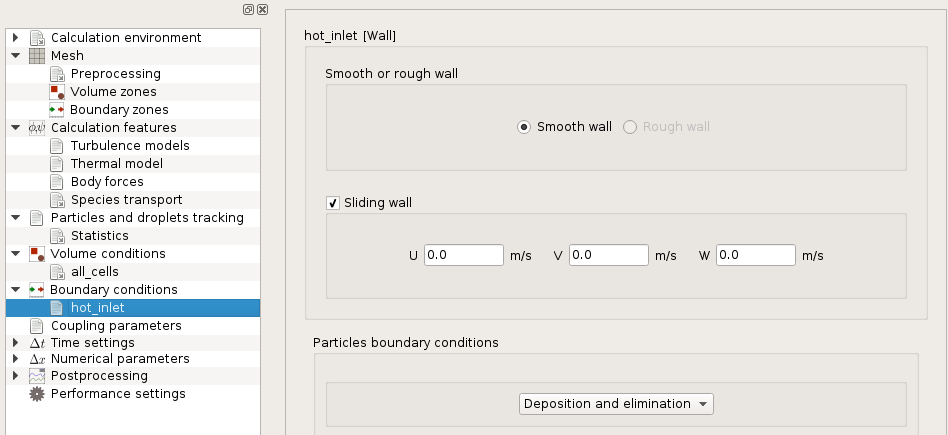
\includegraphics[width=0.9\textwidth]{gui_lagr_bc}
\caption{Lagrangian module - boundary conditions}
\label{fig:CL-Lag}
\end{center}
\end{figure}

%==================================
\subsubsection{Advanced particle-tracking set-up}
%==================================

In this section, some information is provided for a more advanced numerical set-up of a particle-tracking simulation.

\minititre{User-defined stochastic differential equations}
%-------------------------------------------------

\noindent
An adaptation in the \texttt{cs\_user\_lagr\_sde} function is required if
supplementary user variables are added to the particle state vector.
This function is called at each Lagrangian sub-step.

\noindent
The integration of the stochastic differential equations associated with
supplementary particulate variables is done in this function. \\
When the integration scheme of the stochastic differential equations is
a first-order (\texttt{nordre} = 1), this subroutine is called once every
Lagrangian iteration, if it is a second-order (\texttt{nordre} = 2), it is called
twice. \\

\noindent
The solved stochastic differential equations must be written in the
form:
\begin{displaymath}
\frac{d \Phi_p}{dt} \,=\, - \frac{\Phi_p - \Pi}{\tau_\phi}
\end{displaymath}
where $\Phi_p$ is the I\textit{th} supplementary user variable,
$\tau_\phi$ is a quantity homogeneous to a characteristic time, and $\Pi$ is
a coefficient which may be expressed as a function of the other
particulate variables. \\
In order to do the integration of this equation, the following
parameters must be provided:
\begin{list}{-}{}
\item $\tau_\phi$, equation characteristic time
      every particle,
\item $\Pi$ , equation coefficient. If the
      integration scheme is a first-order, then $\Pi$ is expressed as a
      function of the particulate variables at the previous iteration,
      stored in the array \texttt{eptpa}. If the chosen scheme is a second-order,
      then $\Pi$ is expressed at the first call of the function
      (prediction step) as a function of the variables at the
      previous iteration, then at the second call
      (correction step) as a function of the predicted variables.
\end{list}

\noindent
If necessary, the thermal characteristic time $\tau_c$, whose calculation can be modified by the user in the function
\texttt{cs\_user\_lagr\_rt}.

\minititre{User-defined particle relaxation time}
%-------------------------------------------------

\noindent
The particle relaxation time may be modified in the \texttt{cs\_user\_lagr\_rt} function according to the chosen formulation of the drag coefficient. The particle relaxation time, modified or not by the user, is available in the array \texttt{taup}.

\minititre{User-defined particle thermal characteristic time}
%-------------------------------------------

\noindent
The particle thermal characteristic time may be modified in the \texttt{cs\_user\_lagr\_rt\_t} function according to the chosen correlation for the calculation of the
Nusselt number. This function is called at each Lagrangian sub-step.


%==================================
\subsection{Compressible module}
%==================================

When the compressible module\footnote{For more details concerning the
compressible version, the user may refer to the theory guide \cite{theory} and the document ``Implantation
d'un algorithme compressible dans \CS'', Rapport EDF 2003,
HI-83/03/016/A, P. Mathon, F. Archambeau et J.-M. H\'erard.} is
activated, it is recommended to:
\begin{list}{-}{}
 \item use the option ``time step variable in time and uniform in
       space'' (\texttt{idtvar}=1) with a maximum Courant number of 0.4
       (\texttt{coumax}=0.4): these choices must be written in \texttt{cs\_user\_parameters.f90}
       or specified with the GUI.
 \item keep the convective numerical schemes proposed by default (\textit{i.e.}: upwind scheme).
\end{list}
With the compressible algorithm, the specific total energy is a new solved variable
\texttt{isca(ienerg)}). The temperature variable deduced from the specific
total energy variable is \texttt{isca(itempk)} for the compressible module.\\
Initialisation of the options of the variables, boundary conditions, initialisation of the variables and
management of variable physical properties can be done with the GUI. We describe below the subroutines
the user has to fill in without the GUI.

%==================================
\subsubsection{ Initialisation of the options of the variables}
%==================================
\label{prg_uscfx12}%
\noindent
\textit{Subroutines called at each time step.}

When the GUI is not being used, the subroutines \texttt{uscfx1} and \texttt{uscfx2} in \texttt{cs\_user\_parameters.f90}
must be completed by the user.

\texttt{uscfx1} allows to specify:
\begin{list}{-}{}
\item \texttt{ieos}: equation of state (only perfect gas with a constant adiabatic coefficient,
                      \texttt{ieos=1} is available, but the user can complete the subroutine
                      \texttt{cs\_cf\_thermo}, which is not a user subroutine, to add new equations of state).
\item \texttt{call field\_set\_key\_int(ivarfl(isca(itempk)), kivisl, ...)}: molecular thermal conductivity, constant (\texttt{-1}) or variable (\texttt{0}).
\item  \texttt{iviscv}: volumetric molecular viscosity, constant (\texttt{0}) or variable (\texttt{1}).
\end{list}

\texttt{uscfx2} allows to specify:
\begin{list}{-}{}
  \item \texttt{ivivar}: molecular viscosity, constant (\texttt{0}) or variable (\texttt{1}).
  \item \texttt{field\_set\_key\_double(icavr(isca(itempk)), kvisl0, ...)}: reference molecular thermal conductivity.
  \item \texttt{viscv0}: reference volumetric molecular viscosity.
  \item \texttt{xmasmr}: molar mass of the perfect gas (\texttt{ieos=1}).
  \item \texttt{icfgrp}: specify if the hydrostatic equilibrium must be accounted for in the
                         boundary conditions.
\end{list}

%==================================
\subsubsection{Management of the boundary conditions}
%==================================

\noindent
\textit{Subroutine called at each time step.}

When running the compressible module without a GUI, the \texttt{cs\_user\_boundary\_conditions} subroutine can be used to define specific boundary conditions
(see the \texttt{cs\_user\_boundary\_conditions-compressible} file in the directory \texttt{EXAMPLES}
for examples of boundary conditions with the compressible module).

With the compressible module, the following types of boundary condition are avaliable:

\begin{list}{-}{}
  \item Inlet/outlet for which velocity and two thermodynamics variables are known.
  \item Subsonic inlet with imposed total pressure and total energy.
  \item Subsonic outlet with imposed static pressure.
  \item Supersonic outlet.
  \item Wall (adiabatic or not).
  \item Symmetry.
\end{list}

It is advised to only use these predefined boundary conditions type for the compressible module.

%==================================
\subsubsection{Initialisation of the variables}
%==================================

\noindent
\textit{Subroutine called only at the initialisation of the calculation}

When the GUI is not used, the subroutine \texttt{cs\_user\_initialization} is used
initialize the velocity, turbulence and passive scalars (see
the \texttt{cs\_user\_initialization-compressible} file in the directory \texttt{EXAMPLES}
for examples of initialisations with the compressible module). Concerning
pressure, density, temperature and specific total energy, only 2 variables out
of these 4 are independent. The user may then initialise the desired variable pair
(apart from temperature-energy) and the two other variables will be
calculated automatically by giving the right value to the variable
\texttt{ithvar} used for the call to the \texttt{cs\_cf\_thermo} routine.

%==================================
\subsubsection{Management of variable physical properties}
%==================================

\noindent
\textit{Subroutine called at each time step.}

Without the GUI, all of the laws governing the physical properties of the fluid
(molecular viscosity, molecular volumetric viscosity, molecular thermal conductivity and
molecular diffusivity of the user-defined scalars) can be specified in the subroutine \texttt{usphyv} of
the \texttt{cs\_user\_physical\_properties} file,
which is then called at each time step. This subroutine replaces and is similar to \texttt{usphyv}.

The user should check that the defined laws are valid for
the whole variation range of the variables. Moreover, as only the perfect gas with a constant
adiabatic coefficient equation of state is available, it is not advised to give a law for the isobaric
specific heat without modifying the equation of state in the subroutine \texttt{cs\_cf\_thermo} which is not
a user subroutine.

%==================================
\subsection{Management of the electric arcs module}
%==================================

%==================================
\subsubsection{Activating the electric arcs module}\label{sec:acti-lag}
%==================================

The electric arcs module is activated either:
%
\begin{itemize}
 \item [$\bullet$] in the Graphical User Interface (GUI): \texttt{Calculation features} $\rightarrow$ \texttt{Electrical models}
 \item [$\bullet$] or in the user subroutine \texttt{usppmo}, by setting the \texttt{ielarc} or \texttt{ieljou} parameter to a non-null value.
\end{itemize}

%==================================
\subsubsection{Initialisation of the variables}
%==================================

\noindent
\textit{Subroutine called only at initialisation of the calculation}

The subroutine \texttt{cs\_user\_initialization} allows the user to initialise some of the specific physics variables prompted via \texttt{usppmo}. It is called only during the initialisation of the calculation. As usual,the user has access to many geometric variables so
 that the zones can be treated separately if needed.

The values of potential and its constituents are initialised if required.

It should be noted that the enthalpy is relevant.

\begin{list}{-}{}
\item For the electric arcs module, the enthalpy value is taken from the temperature
 of reference \texttt{t0} (given in \texttt{cs\_user\_parameters.c})
 from the temperature-enthalpy tables supplied in the data file \texttt{dp\_ELE.}
 The user must not intervene here.
\item For the Joule effect module, the value of enthalpy must be specified by the user.
 Examples of temperature to enthalpy conversion are given in
 \texttt{cs\_user\_physical\_properties.c}). If not defined, a simple default
 law is used ($H = C_p T$).
\end{list}

%==================================
\subsubsection{Variable physical properties}
%==================================

All the laws of the variation of physical data of the fluid are written (when necessary)
in the subroutine \texttt{cs\_user\_physical\_properties}. It is called at each time step.

{\em WARNING: For the electric module, it is here that all the physical variables are defined
 (including the relative cells and the eventual user scalars):} \texttt{cs\_user\_physical\_properties} {\em {is not used.}}

The user should ensure that the defined variation laws are valid for the whole range of
variables. Particular care should be taken with non-linear laws (for example, a
 $3^{rd}$ degree polynomial law giving negative values of density)

{\em WARNING: In the electric module, all of the physical properties are considered as variables
 and are therefore stored using the \texttt{cs\_field} API. \texttt{cp0}, \texttt{viscls0} and \texttt{viscl0}
 are not used}

For the Joule effect, the user is required to supply the physical properties in the
subroutine. Examples are given which are to be adapted by the user. If the temperature is
to be determined to calculate the physical properties, the solved variable, enthalpy must
 be deduced. The preferred temperature-enthalpy law should be defined
 (a general example is provided in (\texttt{cs\_user\_physical\_properties}),
 and can be used for the initialisation of the variables in
 (\texttt{cs\_user\_initialization})).
 For the electric arcs module, the physical properties are interpolated from the data file
 \texttt{dp\_ELE} supplied by the user. Modifications are generally not necessary.

%==================================
\subsubsection{Boundary conditions}
%==================================

For the electric module,each boundary face in \texttt{cs\_user\_boundary\_conditions} should be associated with a
 \texttt{izone} number \footnote{\texttt{izone} must be less than the maximum
 value allowed by the code, \texttt{nozzppm}. This is fixed at 2000 in \texttt
{ppvar} and cannot be modified.}(the color \texttt{icoul} for example) in
 order to group together all the boundary faces of the same type. In the
 \texttt{cs\_user\_boundary\_conditions} report, the main change from the users point of view concerns the
 specification of the boundary conditions of the potential, which isn't
 implied by default. The Dirichlet and Neumann conditions must be imposed
 explicitly using \texttt{icodcl} and \texttt{rcodcl} (as would be done for
 the classical scalar).

Furthermore, if one wishes to slow down the power dissipation (Joule
effect module) or the current (electric arcs module) from the imposed values
\texttt{(puismp\index{puismp}} and \texttt{couimp\index{couimp}} respectively),
 they can be changed by the potential scalar as shown below:

\begin{list}{-}{}
\item For the electric arcs, the imposed potential difference can be a fixed variable:
 for example, the cathode can be fixed at 0 and the potential at the anode
 contains the variable \texttt{dpot}. This variable is initialised in
in \texttt{cs\_user\_parameters.90}
 by an estimated potential difference. If \texttt{ielcor}=1 (see
 \texttt{cs\_user\_parameters.f90}), \texttt{dpot} is updated automatically during the
 calculation to obtain the required current.
\item For the Joule effect module, \texttt{dpot} is again used with the same
 signification as in the electric arcs module. If \texttt{dpot} is not wanted
 in the setting of the boundary conditions, the variable \texttt{coejou} can be
 used. \texttt{coejou} is the coefficient by which the potential difference is
 multiplied to obtain the desired power dissipation. By default this begins at
 1 and is updated automatically. If \texttt{ielcor}=1 (see \texttt
{cs\_user\_parameters.f90}), multiply the imposed potentials in
\texttt{cs\_user\_boundary\_conditions} by \texttt{coejou} at each time step to
achieve the desired power dissipation.
 \end{list}

 {\em WARNING: In the case of alternating current, attention should be paid to the values of potential
 imposed at the limits: the variable named "real potential" represents an affective
 value if the current is in single phase, and a "real part" if not.}
\begin{list}{-}{}
\item For the Joule studies, a complex potential is sometimes needed
 (\texttt{ippmod(ieljou)}=2): this is the  case in particular where the current
 has three phases. To have access to the phase of the potential, and not just to its
 amplitude, the two variables must be deleted: in \CS, there are two arrays
 specified for this role, the real part and the imaginary
 part of the potential. For use in the code, these variables are named
 ``real potential'' and ``imaginary potential''. For an alternative
 sinusoidal potential $Pp$, the maximum value is noted as $Pp_\text{max}$,
 the phase is noted as $\phi$, the real potential
 and the imaginary potential are respectively $Pp_\text{max}\,cos\phi$ and
$Pp_\text{max}\,sin\phi$.
\item For the Joule studies in which one does not have access to the phases, the real
 potential (imaginary part =0) will suffice (\texttt{ippmod(ieljou)=1}): this is
 obviously the case with
 continuous current, but also with single phase alternative current. In \CS
there is only 1 variable for the potential,  called "real potential". Pay attention to
 the fact that in alternate current, the "real potential" represents a effective value
 of potential , $\frac{1}{\sqrt{2}}\,Pp_\text{max}$ (in continuous current there is no
 such ambiguity).
\end{list}

\minititre{Additions for transformers}

The following additional boundary conditions must be defined for tansformers:
\begin{list}{$\bullet$}{}
\item  the intensity at each electrode
\item  the voltage on each terminal of transformers. To achieve it, the intensity,
 the rvoltage at each termin, the Rvoltage, and the total intensity of the
transformer are calculated.
\end{list}

Finally, a test is performed to check if the offset is zero or if a boundary
 face is in contact with the ground.

%====================================
\subsubsection {Initialisation of the variable options}
%==================================
\label{prg_cs_user_parameters}%

The subroutine \texttt{cs\_user\_parameters} (in \texttt{cs\_user\_parameters.c})
 is called at each time step. It allows:
\begin{list}{$\bullet$}{}
\item to give the coefficient of relaxation of the density \texttt{srrom}:\\
$\rho^{n+1}=\texttt{srrom}*\rho^{n}+(1-\texttt{srrom})\rho^{n}$\\
(for the electric arcs, the sub-relaxation is taken into account during the 2nd time
 step;)

\item to indicate if the data will be fixed in the power dissipation or
 in the current, done in \texttt{ielcor}.
\item target either the current fixed as \texttt{couimp} (electric arcs module)
 or the power dissipation \texttt{puism} (Joule module effect).
\item to fix the initial value of potential difference \texttt{dpot},
 the for the calculations with a single fixed parameter as \texttt{couimp}
 or \texttt{puism}.
\item to define type of scaling model for electric arcs \texttt{modrec}. If scaling
by a resetting plane is choosen then \texttt{idreca} defines the current density component
and \texttt{crit\_reca} the plane used for resetting of electromagnetic variables.
\end{list}

%==================================
\subsection{\CS-\CS coupling}
%==================================

\noindent
\textit{Subroutine called once during the calculation initialisation.}

The user function \texttt{cs\_user\_saturne\_coupling} (in
 \texttt{cs\_user\_coupling.c} is used to couple \CS with itself.
 It is used for turbo-machine applications for instance, the first \CS managing
 the fluid around the rotor and the other the fluid around the stator.
In the case of a coupling between two \CS instances, first argument \texttt{saturne\_name}
 of the function '\texttt{cs\_sat\_coupling\_define}' is ignored.
 In case of multiple couplings, a coupling will be matched with available \CS
 instances based on that argument, which should match the directory name for the
 given coupled domain..\\
The arguments of '\texttt{cs\_sat\_coupling\_define}' are:
\begin{list}{-}{}
\item \texttt{saturne\_name}: the matching \CS application name,
\item \texttt{volume\_sup\_criteria}: the cell selection criteria for support,
\item \texttt{boundary\_sup\_criteria}: the boundary face selection criteria for support (not functional),
\item \texttt{volume\_cpl\_criteria}: the cell selection criteria for coupled cells,
\item \texttt{boundary\_cpl\_criteria}: the boundary face selection criteria for coupled faces,
\item \texttt{verbosity}: the verbosity level.
\end{list}


%==================================
\subsection{Fluid-Structure external coupling}
%==================================

\noindent
\textit{Subroutine called only once}

The subroutine \texttt{usaste} belongs to the module dedicated to external
 Fluid-Structure coupling with \textit{Code\_Aster}. Here one defines the boundary
 faces coupled with \textit{Code\_Aster} and the fluid forces components which are
 given to structural calculation. When using external coupling with \textit{Code\_Aster},
 structure numbers necessarily need to be negative; the references of coupled faces being
 i.e. -1, -2, \emph{etc.}
The subroutine performs the following operations:
\begin{list}{-}{}
 \item '\texttt{getfbr}' is called to get a list of elements matching a
geometrical criterion or reference number then a structure number (negative value) is associated
 to these elements.
 \item the value passed to \texttt{asddlf}, for user-chosen component, for every negative
 structure number, defines the movement imposed to the external structure.
\end{list}
%
\clearpage
%
%==================================
\subsection{ALE module}
%==================================
%==================================
\subsubsection{Initialisation of the options}
%==================================
This initialisation can be performed in the Graphical User Interface (GUI)
 or in the subroutines \texttt{usipph} and \texttt{usstr1}. Firstly,
 when the ``Mobile mesh'' is selected in GUI under the ``Calculation features''
 heading, additional options are displayed. The user must choose the type of mesh
 viscosity and describe its spatial distribution, see \figurename~\ref{fig:Ini-ale}.
%
\begin{figure}[!ht]
\begin{center}
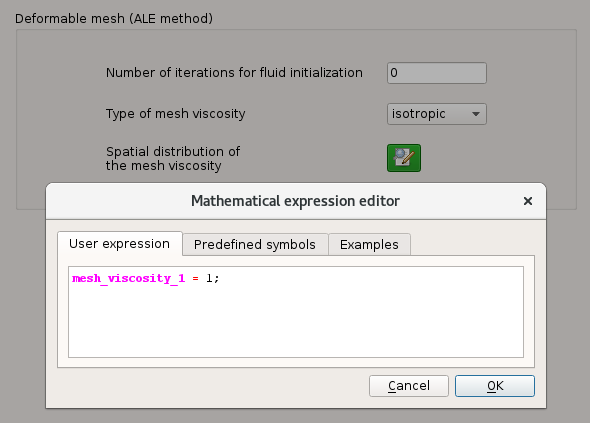
\includegraphics[width=12cm]{gui_ale_mei}
\caption{Thermophysical models - mobile mesh (ALE method)}
\label{fig:Ini-ale}
\end{center}
\end{figure}
%
The following paragraphs are relevant if the GUI is not used.

\minititre{Subroutine \texttt{usipph}}
\noindent
\textit{Subroutine called at the beginning.}
This subroutine completes \texttt{cs\_user\_parameters.f90}.

\texttt{usipph} allows setting options for the ALE module, and in
particular to activate the ALE module (\texttt{iale=1}).

\minititre{Subroutine \texttt{usstr1}}

This subroutine reads in \texttt{cs\_user\_fluid\_structure\_interaction.f90}. It allows to specify the following pieces of information for the structure module:
\begin{list}{-}{}
  \item the index of the structure, (\texttt{idfstr(ifac)} where \texttt{ifac} is the index of the face). Then the total number of structures \texttt{nbstru} is automatically computed by the code. Be careful, the value must belong to 1, ..., \texttt{nbstru}.
  \item the initial value of displacement, velocity and acceleration
    (\texttt{xstr0}, \texttt{xstreq} and \texttt{vstr0}).
\end{list}

Below is a list of the different variables that might be modified:

\begin{list}{$\bullet$}{}

\item{\texttt{idfstr(ifac)}} \\
{the index of the structure, (\texttt{idfstr(ifac)} where \texttt{ifac} is the index of the face), 0 if the face is not coupled to any structure.}

\item{\texttt{xstr0(i,k)}} \\
{initial position of a structure, where \texttt{i} is the dimension of space
and \texttt{k} the index of the structure}

\item{\texttt{xstreq(i,k)}} \\
{equilibrum position of a structure, where \texttt{i} is the dimension of space
and \texttt{k} the index of the structure}

\item{\texttt{vstr0(i,k)}} \\
{initial velicity of a structure, where \texttt{i} is the dimension of space
and \texttt{k} the index of the structure }
\end{list}

%==================================
\subsubsection{Mesh velocity boundary conditions}
%==================================
These boundary conditions can be managed through the Graphical User Interface (GUI)
 or using the subroutine \texttt{usalcl} (called at each time step). With the GUI,
 when the item ``Mobile mesh'' is activated  the item ``Fluid structure interaction''
 appears under the heading ``Boundary conditions''. Two types of fluid-structure
 coupling are offered. The first one is internal, using a simplified structure
 model and the second is external with \textit{Code\_Aster}, see \figurename~
 \ref{fig:CL-ale1} and \figurename~\ref{fig:CL-ale2}.
%
\begin{figure}[ht]
\begin{center}
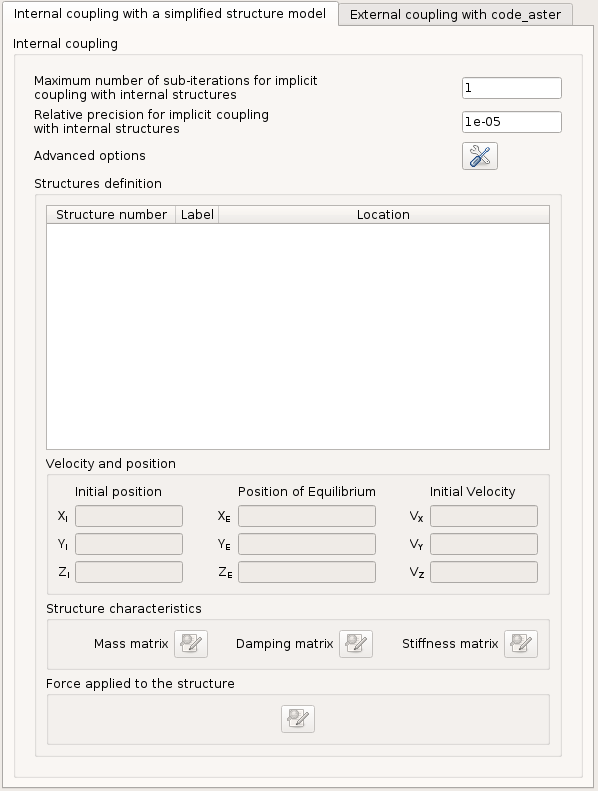
\includegraphics[width=0.9\textwidth]{gui_ale_internal}
\caption{Boundary conditions - internal coupling}
\label{fig:CL-ale1}
\end{center}
\end{figure}
%
\begin{figure}[ht]
\begin{center}
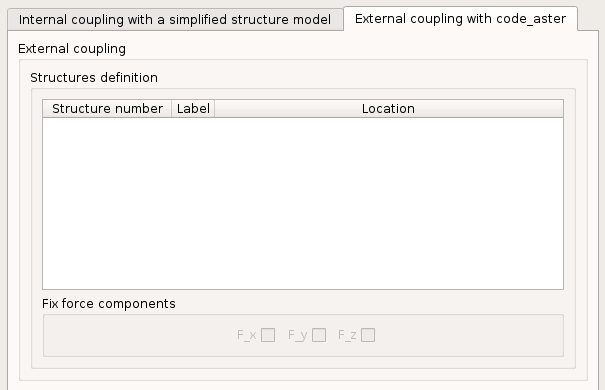
\includegraphics[width=0.9\textwidth]{gui_ale_external}
\caption{Boundary conditions - external coupling}
\label{fig:CL-ale2}
\end{center}
\end{figure}

\minititre{Subroutine \texttt{usalcl}}
When the GUI is not used, the use of \texttt{usalcl} is mandatory to run
a calculation using
the ale module just as it is in \texttt{cs\_user\_parameters.f90}. It is used the same way as
\texttt{cs\_user\_boundary\_conditions} in the framework of
standard calculations, that is to say a loop on the boundary faces
marked out by their colour (or more generally by a property of their
family), where the type of mesh velocity boundary condition is definied for
each variable.

The main numerical variables are described below.

\variab{ialtyb}{ialtyb(nfabor)}{ia}{In the ale module, the user
defines the mesh velocity from the colour of the boundary faces, or
more generally from their properties (colours, groups, ...), from the
boundary conditions defined in \texttt{cs\_user\_boundary\_conditions}, or even from their
coordinates. To do so, the array \texttt{ialtyb(nfabor)} gives for each face
\texttt{ifac} the mesh velocity boundary condition types marked out by the key
words \texttt{ivimpo\index{ivimpo}}, \texttt{igliss\index{igliss}},
\texttt{ibfixe\index{ibfixe}} or \texttt{ifresf\index{ifresf}}}.

\begin{list}{$\bullet$}{}

\item If \texttt{ialtyb(ifac) = ivimpo}: imposed velocity.

\begin{list}{$\rightarrow$}{}
\item In the cases where all the nodes of a face have a imposed displacement,
 it is not necessary to fill the tables with mesh velocity boundary conditions
 for this face, these will be erased. In the other case,
 the value of the Dirichlet must be given in \texttt{rcodcl(ifac,ivar,1)} for
 every value of \texttt{ivar} (\texttt{iuma}, \texttt{ivma} and \texttt{iwma}).
 The other boxes of \texttt{rcodcl} and \texttt{icodcl} are completed automatically.

 The tangential mesh velocity is taken like a tape speed under the
 boundary conditions of wall for the fluid, except if wall fluid velocity
 was specified by the user in the interface or \texttt{cs\_user\_boundary\_conditions} (in which case
 it is this speed which is considered).
\end{list}

 \item if \texttt{ialtyb(ifac) = ibfixe}: fixed wall
\begin{list}{$\rightarrow$}{}
 \item the velocity is null.
\end{list}

 \item if \texttt{ialtyb(ifac) = igliss}: sliding wall
\begin{list}{$\rightarrow$}{}
\item symmetry boundary condition on the mesh velocity vector, which means a homogeneous Neumann on the tangential mesh velocity and a zero Dirichlet on the normal mesh velocity.
\end{list}

 \item if \texttt{ialtyb(ifac) = ifresf}: free-surface
\begin{list}{$\rightarrow$}{}
\item an imposed mesh velocity such that the fluid mass flux is equal to the mesh displacement in order to mimic the free-surface automatically. Note that the boundary condition on the fluid velocity must be set separately (homogeneous Neumann condition for instance).
\end{list}

\end{list}

%==================================
\subsubsection{Modification of the mesh viscosity}
%==================================

The user subroutine \texttt{cs\_user\_physical\_properties} can be used along the ALE (Arbitrary Lagrangian Eulerian
 Method) module, and allows modifying the mesh viscosity.
 It is called before the time loop, and before reading restart files
 (so the mesh is always in its initial position at this stage).
The user can modify mesh viscosity values to prevent cells and nodes from huge
 displacements in awkward areas, such as boundary layer for example.

Note that for more complex settings, the mesh viscosity could be modified in
 \texttt{cs\_user\_initialization} or \texttt{cs\_user\_extra\_operations}.
 The matching field's name is \texttt{mesh\_viscosity}.

%==================================
\subsubsection{Fluid - Structure internal coupling}\label{sec:ALE}
%==================================

In the subroutine \texttt{cs\_user\_fluid\_structure\_interaction} the user provides the parameters of two other subroutines.
\texttt{usstr1} is called at the beginning of the calculation. It is used to define
 and initialise the internal structures where fluid-Structure coupling occurs.
For each boundary face \texttt{ifac}, \texttt{idfstr(ifac)} is the index of the structure
 the face belongs to (if \texttt{idfstr(ifac)} = 0, the face \texttt{ifac} doesn't belong
 to any structure). When using internal coupling, structure index necessarily must be
 strictly positive and smaller than the number of structures. The number of "internal" structures is automatically defined with the maximum
 value of the \texttt{idfstr} table, meaning that internal structure numbers must be defined
 sequentially with positive values, beginning with integer value '1'.

For each internal structure the user can define:
\begin{list}{-}{}
 \item an initial velocity \texttt{vstr0}
 \item an initial displacement \texttt{xstr0} ({\em i.e.} \texttt{xstr0} is the value of the
 displacement \texttt{xstr} compared to the initial mesh at time t = 0)
 \item a displacement compared to equilibrium  \texttt{xstreq} (i.e. \texttt{xstreq}
 is the initial displacement of the internal structure compared to its position at
 equilibrium; at each time step t and for a displacement \text{xstr}(t), the associated
 internal structure will undergo a force $-k*(\text{}t+XSTREQ)$ due to the spring).
\end{list}
\text{xstr0} and \text{vstr0} are initialised with the value 0.
When starting a calculation using ALE, or re-starting a calculation with ALE, based
 on a first calculation without ALE, an initial iteration 0 is automatically performed
 in order to take initial arrays \text{xstr0}, \text{vstr0} and \text{xstreq} into
 account. In any other case, add the following expression '\text{italin=1}' in subroutine
 \text{usipsu}, so that the code can deal with the arrays \text{xstr0}, \text{vstr0} and \text{xstreq}.

When \texttt{ihistr} is set to 1, the code writes in the output the history of the
 displacement, of the structural velocity, of the structural acceleration and of the
 fluid force. The value of structural history output step is the same as the one for
 standard variables \text{nthist}.

The second subroutine, \text{usstr2}, is called at each iteration. One defines in this
 subroutine structural parameters (considered as potentially time dependent): {\em i.e.},
 mass m \text{xmstru}, friction coefficients c \text{xcstru}, and stiffness k \text{xkstru}.
 \text{forstr} array gives fluid stresses acting on each internal structure. Moreover it is also
 possible to take external forces (gravity for example ) into account.
\begin{list}{.}{}
 \item the \text{xstr} array indicates the displacement of the structure compared to its position in the initial mesh,
 \item the \text{xstr0} array gives the displacement of the structures in the initial mesh
 compared to structural equilibrium,
 \item the \text{vstr} array stands for structural velocity.
\end{list}
\text{xstr}, \text{xstr0} and \text{vstr} are \text{DATA} tables that can be used to
 define the  Mass, Friction and Stiffness arays. These are not to be modified.

The 3D structural equation that is solved is the following one:
\begin{equation}\label{eq:FluidStruct}
\displaystyle
\tens{m}.\partial_{tt}\vect{x}+\tens{c}.\partial_{t}\vect{x}+\tens{k}.\left(\vect{x}+\vect{x_0}\right)=\vect{f},
\end{equation}
where $x$ stands for the structural displacement compared to initial mesh position
 \text{xstr}, $x_0$ represents
 the displacement of the structure in initial mesh compared to equilibrium.
Note that $\tens{m}$,$\tens{c}$, and $\tens{k}$ are 3\text{x}3 matrices.
Equation \eqref{eq:FluidStruct} is solved using a Newmark HHT algorithm.
Note that the time step used to solve this equation, \text{dtstr}, can be
 different from the one of fluid calculations. The user is free to define \text{dtstr}
 array. At the beginning of the calculation \text{dtstr} is initialised to the value of
 \text{dtcel} (fluid time step).

%==================================
\subsection{Management of the structure property}
%==================================

The use of \texttt{usstr2} is mandatory to run a calculation using the ALE
 module with a structure module. It is called at each time step.

For each structure, the system that will be solved is:

\begin{equation}
M.x^{''}+C.x^{'}+K.(x-x_{0}) = 0
\end{equation}

where

\begin{list}{-}{}
 \item $M$ is the mass structure (\texttt{xmstru}).
 \item $C$ is the damping coefficient of the structure (\texttt{xcstru}).
 \item $K$ is the spring constant or force constant of the structure (\texttt{xkstru}).
 \item $x_{0}$ is the initial position.
\end{list}

Below is a list of the different variables that might be modified:

\begin{list}{$\bullet$}{}

\item{\texttt{xmstru(i,j,k})} \\
{mass matrix of the structure, where \texttt{i},\texttt{j} is
the array of mass structure and \texttt{k} the index of the structure.}

\item{\texttt{xcstru(i,j,k})}\\
{damping matrix coefficient of the structure, where \texttt{i},\texttt{j} is the array of
damping coefficient and \texttt{k} the index of the structure.}

\item{\texttt{xkstru(i,j,k)}}\\
{spring matrix constant of the structure, where \texttt{i},\texttt{j} is the array of spring
constant and \texttt{k} the index of the structure.}

\item{\texttt{forstr(i,k)}}\\
{force vector of the structure, where \texttt{i} is the force vector and
\texttt{k} the index of the structure.}
\end{list}

%===========================================================
\subsection{Management of the atmospheric module}
%===========================================================

This section describes how to set a calculation using the atmospheric module
of \CS. Each paragraph describes a step of the data setting process.

\subsubsection{Directory structure}\label{sec:atmo_struct}
%
The flowchart (\figurename~\ref{fig:organisation}) recalls the directory
structure of a study generated by \CS (see also \ref{sec:prg_architecture}).
When using the atmospheric module, the structure is identical but a file called
\texttt{meteo} may be added to the data settings in order to provide vertical
profiles of the main variables. This file should be put in the \texttt{DATA}
directory. For more details about the \texttt{meteo} file, see \S~
~\ref{sec:atmo_BCs}).
%
\begin{figure}[ht]
 \centerline{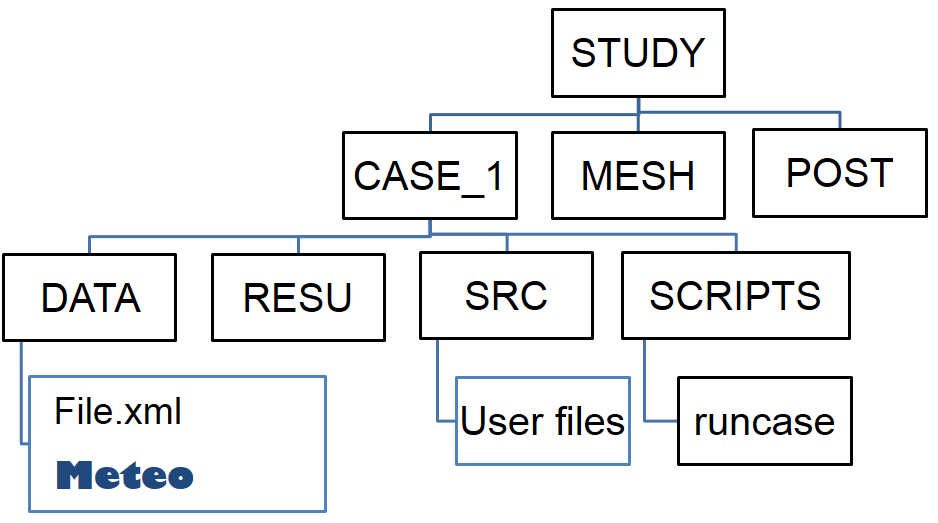
\includegraphics[width=0.6\textwidth]{gui_atmospheric_user_s_guide_v91.png}}
 \caption{Organization of a study (specific files of atmospheric version in bold type)}
 \label{fig:organisation}
\end{figure}
%
\subsubsection{The atmospheric mesh features}
%
An atmospheric mesh has the following specific features:
%
\begin{itemize}
\item The boundary located at the top of the domain should be a plane.
So, horizontal wind speed at a given altitude can be prescribed at the top
face as an inlet boundary.
\item Cells may have very different sizes, from very small (near ground or
buildings) to very large (near the top of domain or far from zone of interest).
\item Vertical resolution: from tiny cells (e.g. $\Delta $\upshape z = 1 m) near
the ground to a few hundreds of meters at the top.
\item Horizontal resolution: from a few meters to hundreds of meters.
\item The length ratio between two adjacent cells (in each direction) should
preferably be between $0.7$ and $1.3$.
\item The z axis represents the vertical axis.
\end{itemize}
%
A topography map can be used to generate a mesh. In this case, the preprocessor
 mode is particularly useful to check the quality of the mesh (run type Mesh
quality criteria).
%
\subsubsection{Atmospheric flow model and steady/unsteady algorithm}
%
The Graphical User Interface (GUI) may be used to enable the atmospheric flow
module and set up the following calculation parameters in the
\texttt{Thermophysical models}-\texttt{Calculation features} page
(see \figurename~\ref{fig:steady}):
%
\subsubsubsection{The atmospheric flow model}
%
The user can choose one of the following atmospheric flow models:
%
\begin{itemize}
\item \textbf{Constant density}: To simulate neutral atmosphere.
\item \textbf{Dry atmosphere}: To simulate dry, thermally-stratified
atmospheric flows (enables \texttt{Potential temperature} as thermal model).
\item \textbf{Humid atmosphere}: To simulate thermally stratified atmospheric
flows (air-water mixture) with phase changes (enables \texttt{Liquid potential
temperature} as thermal model). The model is described in
Bouzereau \cite{bouzereau}.
\end{itemize}
%
\subsubsubsection{The time algorithm}
%
\begin{itemize}
\item Steady flow algorithm: is the one usually set. It sets a time step
variable in space and time. It has to be selected if constant boundary
conditions are used.
\item Unsteady flow algorithm has to be selected for time varying boundary
conditions (the time step can then be variable in time or constant).
\end{itemize}
%
\begin{figure}[ht]
\centerline{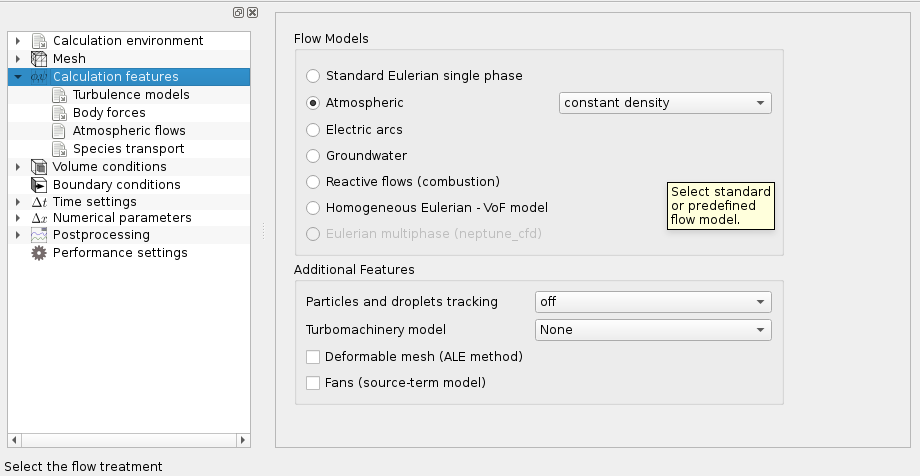
\includegraphics[width=0.7\textwidth]{gui_atmospheric_user_s_guide_v92.png}}
\caption{Selection of atmospheric model}
\label{fig:steady}
\end{figure}
%
\begin{figure}[ht]
\centerline{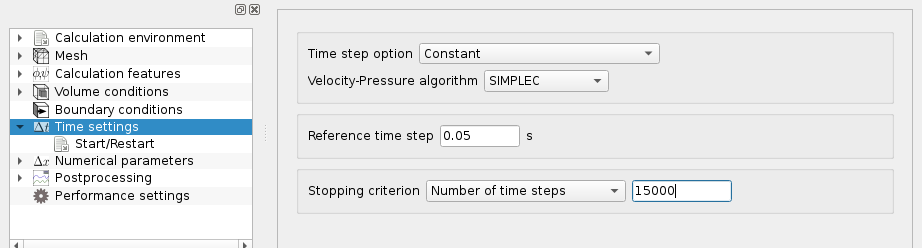
\includegraphics[width=0.9\textwidth]{gui_atmospheric_user_s_guide_v93.png}}
\caption{Selection of steady/unsteady flow algorithm}
\label{fig:global}
\end{figure}
%
Table \tablename~\ref{tab:param_list} can help to choose the right parameters
depending on the type of atmospheric flow.
%
\subsubsubsection{Warnings}
The following points have to be considered when setting the parameters
described above:
\begin{itemize}
\item The potential temperature thermal model and the liquid potential
temperature one (see the paragraph ``Atmospheric main variables'' for the
definition) requires that the vertical component of the gravity is set to
$g_z=-9.81 m.s^{-2}$ ($g_x=g_y=0 m.s^{-2}$),
otherwise pressure and density won't be correctly computed.
\item As well, the use of scalar with drift for atmospheric dispersion requires
the gravity to be set to $g_z=-9.81$ ($g_x=g_y=0 m.s^{-2}$), even if the density
is constant.
\end{itemize}
%
\subsubsection{Physical properties}
%
The specific heat value has to be set to the atmospheric value
$C_{p}=1005 J/kg/K$.
%
\begin{table}[ht]\label{tab:param_list}
\begin{center}
\begin{tabular}{|p{80pt}|p{70pt}|p{70pt}|p{80pt}|p{100pt}|}
\hline
\textbf{Parameters} & \textbf{Constant density} & \textbf{Dry atmosphere} & \textbf{Humid atmosphere} & \textbf{Explanation} \\
\hline
pressure boundary condition & Neumann first order & Extrapolation & Extrapolation &
In case of \textbf{Extrapolation}, the pressure gradient is assumed (and set) constant, whereas in case of \textbf{Neumann first order},
the pressure gradient is assumed (and set) to zero. \\
\hline
Improved pressure interpolation in stratified flows & no & yes & yes & If yes, exact balance between the hydrostatic part of the pressure gradient and the gravity term $\rho g$ is numerically ensured. \\
\hline
Gravity (gravity is assumed aligned with the z-axis) & $g_z=0$ or $g_z=-9.81 m.s^{-2}$ (the latter is useful for scalar with drift) & $g_z=-9.81 m.s^{-2}$ & $g_z=-9.81 m.s^{-2}$ &  \\
\hline
Thermal variable & no & potential temperature & liquid potential temperature &  \\
\hline
Others variables & no & no & total water content, droplets number &  \\
\hline
\end{tabular}\label{tab1}
\caption[List of parameters]{List of parameters}
\end{center}
\end{table}
%
\subsubsection{Boundary and initial conditions}\label{sec:atmo_BCs}
%
The \texttt{meteo} file can be used to define initial conditions for the
different fields and to set up the inlet boundary conditions. For the velocity
field, \CS can automatically detect if the boundary is an inlet boundary or an
outflow boundary, according to the wind speed components given in the
\texttt{meteo} file with respect to the boundary face orientation. This is often
used for the lateral boundaries of the atmospheric domain, especially if the
profile is evolving in time. In the case of inlet flow, the data given in the
\texttt{meteo} file will be used as the input data (Dirichlet boundary condition)
for velocity, temperature, humidity and turbulent variables. In the case of
outflow, a Neumann boundary condition is automatically imposed (except for the
pressure). The unit of temperature in the \texttt{meteo} file is the degree
Celsius whereas the unit in the GUI is the kelvin.

To be taken into account, the \texttt{meteo} file has to be selected in the GUI
(\texttt{Atmospheric flows} page, see \figurename~\ref{fig:meteo}) and the check
box on the side ticked. This file gives the profiles of prognostic atmospheric
variables containing one or a list of time stamps. The file has to be put in the
\texttt{DATA} directory.
%
\begin{figure}[htbp]
\centerline{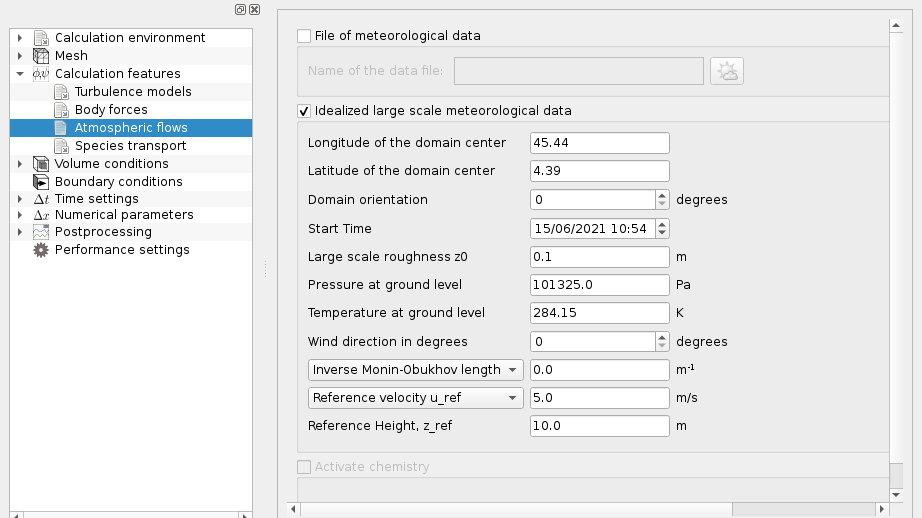
\includegraphics[width=0.9\textwidth]{gui_atmo_read.png}}
\caption{Selection of the \texttt{meteo} file}
\label{fig:meteo}
\end{figure}
%
An example of file \texttt{meteo} is given in the directory
\texttt{DATA/REFERENCE/}. The file format has to be strictly respected.
The horizontal coordinates are not used at the present time (except when
boundary conditions are based on several meteorological vertical profiles)
and the vertical profiles are defined with the altitude above sea level. The
highest altitude of the profile should be above the top of the simulation domain
and the lowest altitude of the profile should be below or equal to the lowest
level of the simulation domain. The line at the end of the \texttt{meteo} file
should not be empty.

If the boundary conditions are variable in time, the vertical profiles for
the different time stamps have to be written sequentially in the \texttt{meteo}
file.

You can also set the profiles of atmospheric variables directly in the GUI.
The following boundary conditions can be selected in the GUI:
%
\begin{itemize}
\item Inlet/Outlet is automatically calculated for lateral boundaries
(e.g. North, West\textellipsis ) of the computational domain
(see \figurename~\ref{fig:inlet}).
\item Inlet for the top of the domain (see \figurename~\ref{fig:top}).
\item Rough wall for building walls (see \figurename~\ref{fig:walls}) or for
the ground (see \figurename~\ref{fig:ground}).
The user has to enter the roughness length. In case of variable roughness
length, the user has to provide the land use data and the association
between the roughness length values and land use categories.
\end{itemize}
%
\begin{figure}[htbp]
\centerline{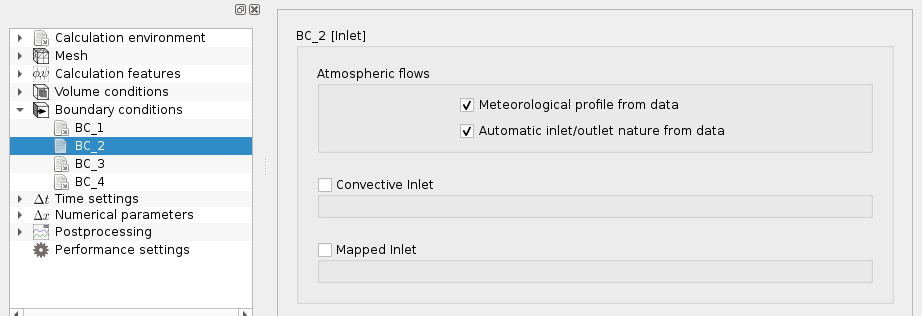
\includegraphics[width=0.9\textwidth]{gui_atmospheric_user_s_guide_v95.png}}
\caption{Selection of automatic inlet/ outlet for boundary conditions }
\label{fig:inlet}
\end{figure}
%
\begin{figure}[htbp]
\centerline{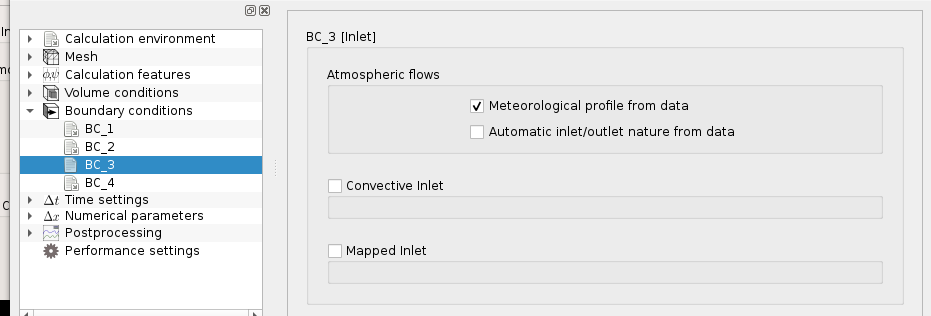
\includegraphics[width=0.9\textwidth]{gui_atmospheric_user_s_guide_v96.png}}
\caption{Selection of the boundary condition for the top of the domain }
\label{fig:top}
\end{figure}
%
\begin{figure}[htbp]
\centerline{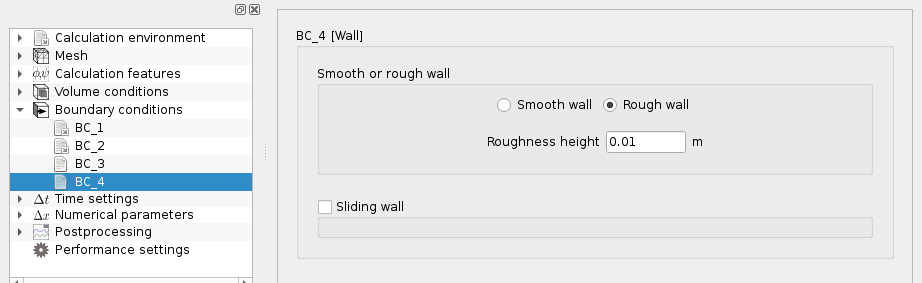
\includegraphics[width=0.9\textwidth]{gui_atmospheric_user_s_guide_v97.png}}
\caption{Selection of the boundary condition for building walls}
\label{fig:walls}
\end{figure}
%
\begin{figure}[htbp]
\centerline{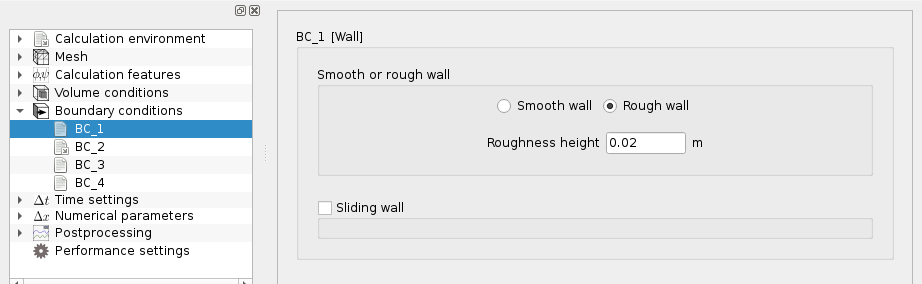
\includegraphics[width=0.9\textwidth]{gui_atmospheric_user_s_guide_v98.png}}
\caption{Selection of the boundary condition for the ground}
\label{fig:ground}
\end{figure}

\paragraph{Remark:} If a meteorological file is given, it is used by default to
initialize the variables. If a meteorological file is not given, the user can
use the standard \CS initial and boundary conditions set up but has to be aware
that even small inconsistencies can create very large buoyancy forces and
spurious circulations.

\subsubsubsection{Boundary conditions based on several meteorological vertical profiles}

In some cases, especially when outputs of a mesoscale model are used, you
need to build input boundary conditions from several meteorological vertical
wind profiles. Cressman interpolation is then used to create the boundary
conditions. The following files need to be put in the \texttt{DATA} directory:
\begin{itemize}
\item All \texttt{meteo} files giving the different vertical profiles of
prognostic variables (wind, temperature, turbulent kinetic energy and
dissipation).
\item A file called \texttt{imbrication\_files\_list.txt} which is a list
of the \texttt{meteo} files used.
\item A separate \texttt{meteo} file which is used for the initial conditions
and to impose inlet boundary conditions for the variables for which Cressman
interpolation is not used (for example: temperature, turbulent kinetic energy).
This file must follow the rules indicated previously.
\end{itemize}
The following files should be put in the SRC directory:
\begin{itemize}
\item The user source file \texttt{cs\_user\_parameters.f90}. In this file, set
the \texttt{cressman\_} flag of each variable, for which the Cressman
interpolation should be enabled, to \texttt{.true.}.
\end{itemize}
%
\subsubsection{User subroutines}
%
The user subroutines are used when the graphical user interface is not
sufficient to set up the calculation. We give some examples of user file for
atmospheric application:
\begin{itemize}
\item \texttt{cs\_user\_source\_terms.f90}: to add a source term in the
prognostic equations for forest canopy modelling, wind turbine wake modelling...
See the associated \doxygenfile{cs_user_source_terms.html}{\texttt{doxygen} documentation
for examples of use of \texttt{cs\_user\_source\_terms.f90}}.
\item \texttt{cs\_user\_parameters.f90}: to activate the Cressman interpolation.
For example, it is used to impose inhomogeneous boundary conditions. See the associated
\doxygenfile{f_parameters.html}{\texttt{doxygen} documentation for examples of use of
\texttt{cs\_user\_parameters.f90}}.
\item \texttt{cs\_user\_extra\_operations-extract.f90}: to generate vertical
profiles for post processing. See the associated
\doxygenfile{cs_user_extra_operations_examples.html}{\texttt{doxygen} documentation
for examples of use of \texttt{cs\_user\_extra\_operations.f90}}.
\item \texttt{cs\_user\_boundary\_conditions-atmospheric.f90}: show how to set
up the boundary conditions and to put a heterogeneous roughness length...
See the associated \doxygenfile{cs_user_boundary_conditions_examples.html}{\texttt{doxygen}
documentation for examples of use of \texttt{cs\_user\_boundary\_conditions.f90}}.
\end{itemize}
%
\paragraph{Remark:}
If the computation is set without the GUI, other user subroutines such as the
following have to be used:
\begin{itemize}
\item \texttt{cs\_user\_initialization-atmospheric.f90}: allows to initialize
or modify (in case of a restarted calculation) the calculation variables and
the values of the time step. See the associated
\doxygenfile{user_initialization.html}{\texttt{doxygen} documentation for
examples of use of \texttt{cs\_user\_initialization.f90}}.

\item \texttt{cs\_user\_boundary\_conditions-atmospheric.f90}: allows to define
all the boundary conditions. For each type of boundary condition, faces should
be grouped as physical zones characterized by an arbitrary number \texttt{izone}
chosen by the user. If a boundary condition is retrieved from a meteorological
profile, the variable \texttt{iprofm(izone)} of the zone has to be set to 1.
The vertical profiles of atmospheric variables can be described in this file.
\end{itemize}
%
Examples are available in the directory \texttt{SRC/EXAMPLE}.
%
\subsubsection{Physical models}
%
\subsubsubsection{Atmospheric dispersion of pollutants}
%
To simulate the atmospheric dispersion of pollutant, one first need to define
the source(s) term(s). That is to say the location i.e. the list of cells or
boundary faces, the total air flow, the emitted mass fraction of pollutant,
the emission temperature and the speed with the associated turbulent parameters.
The mass fraction of pollutant is simulated through a user added scalar that
could be a `scalar with drift' if wanted (aerosols for example).

The simulations can be done using 3 different methods:
\begin{enumerate}
\item Using a mass source term, that is added in the Navier-Stokes
equations using the \texttt{cs\_user\_mass\_source\_terms.f90} user subroutine.

\item Prescribing a boundary condition code ``total imposed mass flux`` for
some boundary faces using the \texttt{cs\_user\_boundary\_conditions.f90} user
subroutine.

\item Using a scalar source term. In this case, the air inflow is not taken
into account. The user has to add an explicit part to the equations
for the scalar through the \texttt{cs\_user\_source\_terms.f90} file. This is
done by selecting the cells and adding the source term \texttt{crvexp (cells)}
which equals to the air flux multiplied by the mass fraction, while the
implicit part \texttt{crvimp} is set to zero.
\end{enumerate}

The first method is recommended, but one must take care that each source
influences the dispersion of the others, which is physically realistic. So
if the impact of several sources has to be analyzed independently it has first
to be verified that these influences are negligible or as many simulations
as there are sources have to be run.

With the second method, the same problem of sources interactions appears, and
moreover standard Dirichlet conditions should not be used (use
\texttt{itypfb=i\_convective\_inlet} and \texttt{icodcl=13} instead) as
the exact emission rate cannot be prescribed because the diffusive part
(usually negligible) cannot be quantified. Additionally, it requires that
the boundary faces of the emission are explicitly represented in the mesh.

Finally the third method does not take into account the jet effect of the
emission and so must be used only if it is sure that the emission does not
modify the flow.

Whatever solution is chosen, the mass conservation should be verified by using
for example the
\texttt{cs\_user\_extra\_operations-scalar\_balance\_by\_zone.f90} file.

\subsubsubsection{Soil/atmosphere interaction model}

This model is based on the force restore model (Deardorff \cite{deardorff}).
It takes into account heat and humidity exchanges between the ground and the
atmosphere at daily scale and the time evolution of ground surface temperature
and humidity. Surface temperature is calculated with a prognostic equation
whereas a 2-layers model is used to compute surface humidity.

The parameter \texttt{iatsoil} in the file \texttt{atini0.f90} needs to be equal to one to
activate the model. Then, the source file \texttt{solvar.f90} is used.

Three variables need to be initialized in the file \texttt{atini0.f90}: deep soil
temperature, surface temperature and humidity.

The user needs to give the values of the model constants in the file
\texttt{solcat.f90}: roughness length, albedo, emissivity...

In case of a 3D simulation domain, land use data has to be provided for the domain.
Values of model constants for the land use categories have also to be
provided.

\subsubsubsection{Radiative model (1D)}

The 1D-radiative model calculates the radiative exchange between different
atmospheric layers and the surface radiative fluxes.

The radiative exchange is computed separately for two wave lengths intervals

\begin{itemize}
\item Calculation in the infrared spectral domain (file \texttt{rayir.f90})
\item Calculation in the spectral range of solar radiation (file
\texttt{rayso.f90})
\end{itemize}
This 1D-radiative model is needed if the soil/atmosphere interaction model
is activated.

This model is activated if the parameter \texttt{iatra1} is equal to one in the
file \texttt{cs\_users\_parameters.f90}.

\subsubsection{Atmospheric main variables}

For more details on the topic of atmospheric boundary layers, see  Stull
\cite{stull}.
%
\begin{itemize}
\item Definition of the potential temperature:
\[
\theta =T\left(\frac{P}{P_{r}}\right)^{-\frac{R_{d}}{C_{p}}}
\]
\item Definition of liquid potential temperature:
\[
\theta_{l} = \theta \left( 1-\frac{L}{C_{p}T} q_{l} \right)
\]
\item Definition of virtual temperature:
\[
T_{v} = \left(1+0.61q\right)T
\]
\item Gas law:
\[
P = \rho \frac{R}{M_{d}}\left(1+0,61q\right)T
\]
with $R=R_{d} M_{d}$.
\item Hydrostatic state:
\[
\frac{\partial P}{\partial z} = -\rho g
\]
\end{itemize}
%
\begin{table}[htbp]
\begin{center}
\begin{tabular}{|l|l|l|l|}
\hline
\textbf{Constant name} & \textbf{Symbol} & \textbf{Values} & \textbf{Unit} \\
\hline
Gravity acceleration at sea level & $g$ & $9.81$ & $m.s^{-2}$ \\
\hline
Effective Molecular Mass for dry air & $M_{d}$ & $28.97$ & $kg.kmol^{-1}$ \\
\hline
Standard reference pressure & $P_{r}$ & $10^{5}$ & $Pa$ \\
\hline
Universal gas constant & $R$ & $8.3143$ & $J.K^{-1}.mol$ \\
\hline
Gas constant for dry air & $R_{d}$ & $287$ & $J.kg^{-1}.K^{-1}$ \\
\hline
\end{tabular}\label{tab2}
\end{center}
\caption{Constant name}
\end{table}

\begin{table}[htbp]
\begin{center}
\begin{tabular}{|l|p{113pt}|}
\hline
\textbf{Variable name} &\textbf{Symbol} \\
\hline
Specific heat capacity of dry air & $C_{p}$ \\
\hline
Atmospheric pressure & $P$ \\
\hline
Specific humidity & $q$ \\
\hline
Specific content for liquid water & $q_{l}$ \\
\hline
Temperature & $T$ \\
\hline
Virtual temperature & $T_{v}$ \\
\hline
Potential temperature & $\theta$ \\
\hline
Liquid potential temperature & $\theta_{l}$ \\
\hline
Latent heat of vaporization & $L$ \\
\hline
Density & $\rho $ \\
\hline
Altitude & $z$ \\
\hline
\end{tabular}\label{tab3}
\caption{Variable name}
\end{center}
\end{table}
%
\subsubsection{Recommendations}\label{subsubsec:recommendations}
%
This part is a list of recommendations for atmospheric numerical simulations.
%
\begin{itemize}
\item Enough probes at different vertical levels in the domain should be used
to check the convergence of the calculation.
\item An inflow boundary condition at the top level of the domain should be set
(symmetry and automatic inlet/outlet are not appropriate).
\item A Courant number too small or too big has to be avoided (see \CS Best
Practice Guidelines). That is the reason why the option \texttt{variable time
step in space and in time} is recommended for steady simulations when there are
large differences of cell size inside the domain (which is generally the case
for atmospheric simulations). With this option, it can be necessary to change
the reference time step and the time step maximal increase (by default, the time
step increase rate is $10\%$).
\end{itemize}
%
In some cases, results can be improved with the following modifications:
%
\begin{itemize}
\item In some case, the turbulent eddy viscosity can drop to unrealistically low
values (especially with $k-\varepsilon$ model in stable atmospheric condition).
In those cases, it is suggested to put an artificial molecular viscosity around
$0.1 m^{2}.s^{-1}$.
\item If the main direction of wind is parallel to the boundary of your computing
domain, try to set symmetry boundary conditions for the lateral boundaries to
avoid inflow and outflow on the same boundary zone (side of your domain).
Another possibility is to use a cylindrical mesh.
\item To avoid inflow and outflow on the same boundary zone (side of your domain),
avoid the case of vertical profile in the input data \texttt{meteo} file with
changes of the sign of velocity of wind ($V_x$ or/and $V_y$).
\end{itemize}

%==================================
%\subsection{Cooling tower modelling}
%==================================

%==================================
%\subsubsection{Parameters}
%==================================

%\noindent
%\textit{Subroutine called only during calculation initialisation? OR AT EACH ITERATION?.}

%The subroutine \texttt{uscti1} contains calculation parameters such as:
%\begin{list}{-}{}
% \item  temperature parameters,
% \item  the number of exchange zones at various locations,
% \item  the air properties.
%\end{list}

%==================================
%\subsubsection{Initialisation of the variables}
%==================================

%With the additional variables introduced with the air-cooling module, the
%following quantities may be initialized by  \texttt{cs\_user\_initialization} in
%user selected zones in addition to the usual quantities:
%\begin{list}{-}{}
% \item the air temperature, variable of index \texttt{isca(ihumid)},
% \item the air humidity, variable of index \texttt{isca(itemp4)},
%\end{list}
%where \texttt{iel} can be an element found in a list returned by the routine
% '\texttt{getcel}'.

%==================================
%\subsubsection{Definition of the exchange zones}
%==================================

%The subroutine \texttt{usctdz} is used to define the exchange zones of a cooling
% tower. The user provides the following parameters:
%\begin{list}{-}{}
% \item \texttt{imzech}: its value is related to the model used:
%      \begin{list}{$\rightarrow$}{}
%       \item 0: no model is used,
%       \item 1: Merkel model is used,
%       \item 2: Poppe model is used,
%      \end{list}
% \item 10 exchange zone parameters.
%\end{list}
%These arguments are passed to the subroutine '\texttt{defct}' along with a
%geometrical selection criterion.

%==================================
\subsection{Turbomachinery computations}
%==================================

\subsubsection{Introduction}

Two classical models are available in \CS for rotor/stator
interactions modelling in turbomachinery computations: the steady
approach which is based on the so-called \emph{Frozen Rotor} modelling
and the \emph{transient rotor/stator} approach which is based on a
sliding mesh technique.

\underline{\emph{Warning:}} This section describes these functionalities based on
a single \CS computation. An alternative rotor/stator coupling based
on coupling of boundary conditions is also possible (and only briefly
described in this section) but it is not recommended.

\subsubsection{Meshing reccomendations}\label{tbm_mesh}

\paragraph{Periodicity}\label{tbm_mesh_perio}

The rotational periodicity treatment is possible only in \emph{Frozen
Rotor}. However, the interface plane between rotor and stator
must match in the azimutal $\theta$ direction:
$$\theta_{\text{min}}^{\text{rotor}}(z)=\theta_{\text{min}}^{\text{stator}}(z),\quad\theta_{\text{max}}^{\text{rotor}}(z)=\theta_{\text{max}}^{\text{stator}}(z)$$
for all $z$ through the rotation axis direction.

\paragraph{Rotor/stator interface}\label{tbm_mesh_interface}
\begin{itemize}
\item \emph{Unsteady rotor/stator}: in the input mesh(es), the
  interface between rotor and stator domains has to be composed of
  \underline{boundary faces}. Then the interface boundary faces are joined
  during the computation and become internal faces, as is usual for
  mesh joining in the preprocessing stage. A simple way to ensure
  joining is not done prematurely is to provide
  \underline{separated meshes} for each rotor or stator domain.
\item \emph{Frozen Rotor}: the interface can be composed of boundary
   faces (in which case the interface boundary faces are joined at
   the beginning of the computation) or of internal faces.
\end{itemize}

\paragraph{Meshing of the interface region}\label{tbm_user_bpg_mesh}

As mentioned above, when a rotor/stator interface boundary exists (in
particular for the \emph{unsteady rotor/stator} model), boundary faces
are joined by the solver during the computation, based on the current
rotor position. It is thus important to be aware that the success of
a joining operation is strongly dependant on the
\underline{quality of the mesh at the interface}. More precisely,
the refinement must be as similar as possible at both sides of the
interface. Moreover, it is reminded that the tolerance parameter of
a joining is a fraction of the shortest edge linked with a vertex of
a joined face. Consequently, cells with high aspect ratios where the
refinement in the azimutal $\theta$ direction is much coarser than
those in one of the two others can also lead to a joining failure.
In particular, the user should be careful to avoid elongated
viscous layer type cells in curved areas such as a rotor-stator interface.

If the meshes at both sides of the interface are very different
such that the joining fails, advanced joining parameters are
available. However, modifying the mesh is more likely to
succeed. The introduction of a somekind of buffer cells layer on
both sides of the interface should be very valuable. Ideally, each
of the two layers should have the same refinement and a constant
azimutal step (this latter recommandation is relevant only for
\emph{unsteady rotor/stator} model).

\paragraph{Alternative rotor/stator coupling}\label{tbm_user_bpg_cpl}

If the meshes at both sides of the interface are very different and
can not be modified, a fallback solution is to use the rotor/stator model
based on the boundary conditions coupling.

\underline{\emph{Warning:}} Contrarily to the mesh joining approach, the
boundary conditions coupling approach is not fully conservative.

\subsubsection{Turbomachinery dedicated postprocessing functions}\label{tbm_user_post}

Useful postprocessing functions relative to the machinery
characteristics are available: postprocessing of the couple on the
rotor walls and postprocessing of the head generated by the machinery.

\subsubsection{Data setting, keywords and examples}\label{tbm_date_setting}
Data setting, keywords and examples for turbomachinery computations
(mesh joining or boundary conditions coupling), are provided in
\doxygenfile{turbomachinery.html}{the dedicated \texttt{doxygen}
documentation}.

%==================================
\subsection{Cavitation module}
%==================================

The cavitation module is based on an homogeneous mixture model. The
physical properties (density and dynamic viscosity) of the mixture
depends on a resolved void fraction and constant reference properties
of the liquid phase and the gas phase.

For a description of the user management of the cavitation module,
please refer to \doxygenfile{cavit.html}{the dedicated
  \texttt{doxygen} documentation}.

%-------------------------------------------------------------------------------

% This file is part of code_saturne, a general-purpose CFD tool.
%
% Copyright (C) 1998-2022 EDF S.A.
%
% This program is free software; you can redistribute it and/or modify it under
% the terms of the GNU General Public License as published by the Free Software
% Foundation; either version 2 of the License, or (at your option) any later
% version.
%
% This program is distributed in the hope that it will be useful, but WITHOUT
% ANY WARRANTY; without even the implied warranty of MERCHANTABILITY or FITNESS
% FOR A PARTICULAR PURPOSE.  See the GNU General Public License for more
% details.
%
% You should have received a copy of the GNU General Public License along with
% this program; if not, write to the Free Software Foundation, Inc., 51 Franklin
% Street, Fifth Floor, Boston, MA 02110-1301, USA.

%-------------------------------------------------------------------------------

%==================================
%==================================
\section{Keyword list}
%==================================
%==================================
\label{sec:prg_motscles}

The keywords are classified under relevant headings. For each keyword of \CS Kernel,
the following informations are given:

\noindent
\makebox[2.5cm][l]{Variable name}\makebox[1.3cm][l]{Type}%
\makebox[5cm][l]{Allowed values}%
\makebox[4.cm][l]{[Default]}O/C\hspace{1cm}Level\\
\hspace*{2.5cm}Description\\
\hspace*{2.5cm}Potential dependences


\begin{list}{$\bullet$}{}
\item \textbf{Variable name}: Name of the variable containing the keyword.

\item \textbf{Type}: a (Array), i (Integer), r (Real number), c
      (Character string).

\item \textbf{Allowed values}: list or range of allowed values.

\item \textbf{Default}: value defined by the code before any user
      modification (every keyword has one). In some cases, a
      non-allowed value is given (generally $-999$ or $-10^{12}$), forcing the
      user to specify a value. If he does not do it, the code may:
\begin{list}{-}{}
\item automatically use a recommended value (for example, automatic
      choice of the variables for which chronological records will be
      generated).

\item stop, if the keyword is essential.
\end{list}

\item \textbf{O/C}: Optional/Compulsory
\begin{list}{-}{}
\item O: optional keyword, whose default value may be enough.

\item C: keyword which must imperatively be specified.
\end{list}

\item \textbf{Level}: L1, L2 or L3
\begin{list}{-}{}
\item L1 (level 1): the users will have to modify it in the framework of
      standard applications. The L1 keywords are written in bold.

\item L2 (level 2): the users may have to modify it in the framework of
      advanced applications. The L2 keywords are all optional.

\item L3 (level 3): the developers may have to modify it; it keeps its
      default value in any other case. The L3 keywords are all optional.
\end{list}

\item \textbf{Description}:  keyword description, with its potential
      dependences.

\end{list}

The L1 keywords can be modified through the Graphical Use Interface or
in the \texttt{cs\_user\_parameters.c} file. L2 and L3 keywords can only be modified through
the \texttt{cs\_user\_parameters.c} file, even if they do not appear in the version proposed
as example it the \texttt{SRC/REFERENCE/base} directory.\\
It is however recommended not to modify the keywords which do not belong to the L1
level.

The alphabetical keyword list is displayed in the index, in the end of
this report.

\minititre{Notes}
$\bullet\ $The notation ``d'' refers to a double precision real. For
           instance, 1.8d-2 means 0.018. \\
$\bullet\ $The notation ``{\tt grand}'' (which can be used in the code)
corresponds to $10^{12}$.

%==================================
\subsection{Input-output}
%==================================

\minititre{Notes}
\begin{list}{$\bullet$}{}
\item Two different files can not use the same unit number (in Fortran) nor the
      same name.
\end{list}

%==================================
\subsubsection{''Calculation'' files}
%==================================

\minititre{General}

\minititre{Thermochemistry}

For the calculation file related to the thermochemistry, please refer
to the dedicated \doxygenfile{group__userfile.html}{\texttt{Doxygen} documentation}.

%==================================
\subsection{Numerical options}
%==================================
\subsubsection{Calculation management}
%==================================

The following \doxygenfile{group__time__step__options.html}{\texttt{Doxygen} documentation}
provides information about the various calculation management options available
in \CS such as \texttt{ntmabs}, \texttt{ntcabs}, etc.

%==================================
\subsubsection{Scalar unknowns}
%==================================

Several keywords refering to the scalar unknowns are
detailed in the following
\doxygenfile{structcs__thermal__model__t.html}{\texttt{Doxygen}
documentation}. The \doxygenfile{structcs__stokes__model__t.html}{\texttt{Doxygen} page}
of the Stokes model structure also contains some keywords such as \texttt{icpsyr},
\texttt{iclvfl} or \texttt{itbrrb}.
For other keywords, please refer to the following \texttt{Doxygen} pages refering to
\doxygenanchor{group__main__variables.html\#nscaus}{\texttt{nscaus}} and
\doxygenanchor{group__scalar__params.html\#iscacp}{\texttt{iscacp}}.

%==================================
\subsubsection{Definition of the equations}
%==================================

For informations about \texttt{istat}, \texttt{iconv}, \texttt{idiff}
or \texttt{idifft}, please refer to the following
\doxygenfile{structcs__var__cal__opt__t.html}{\texttt{Doxygen} documentation}.

Moreover, one can find details about the \texttt{idircl} keyword
\doxygenanchor{group__linear__solver.html\#idircl}{here} and about the
\texttt{ivisse} keyword \doxygenanchor{structcs__stokes__model__t.html\#ivisse}{there}.

%==================================
\subsubsection{Definition of the time advancement}
%==================================

\motcleb{idilat}{i}{1, 2, 3, 4}{1}{O}{L1}
{Algorithm to take into account the density variation in time\\
\hspace*{1.3cm}= 1: steady dilatable flow algorithm (default)\\
\hspace*{1.3cm}= 2: unsteady dilatable flow algorithm\\
\hspace*{1.3cm}= 3: low-Mach number algorithm\\
\hspace*{1.3cm}= 4: non conservative algorithm for fire simulation\\
always useful}

\motcleb{cdtvar}{ra}{strictly positive real number}{1}{O}{L1}
{multiplicative factor applied to the time step for each scalar\\
Hence, the time step used when solving the evolution equation for the
variable is the time step used for the dynamic equations (velocity/pressure)
multiplied by {\tt cdtvar}.\\
The size of the array {\tt cdtvar} is {\tt nvar}. For instance, the multiplicative
coefficient applied to the scalar 2 is {\tt cdtvar(isca(2))}). Yet, the value of
{\tt cdtvar} for the velocity components and the pressure is not used. Also,
although it is possible to change the value of {\tt cdtvar} for the turbulent
variables, it is highly not recommended\\
useful if and only if {\tt nscal} $\geqslant$ 1}

\motcle{varrdt}{r}{strictly positive real number}{0.1}{O}{L3}
{maximum allowed relative increase in the calculated time step value
between two successive time steps (to ensure stability, any decrease in the time step
is immediate and without limit)\\
useful if {\tt idtvar} $\ne$ 0}

For details about time stepping options, please refer to the
dedicated \doxygenfile{group__time__step__options.html}{\texttt{Doxygen}
documentation}.

\minititre{Non-constant time step}
The calculation of the time step uses a reference time step {\tt dtref} (at
the calculation beginning). Later, every time step, the time step value
is calculated by taking into account the different existing limits, in
the following order: \\
\hspace*{1.cm}$\bullet$ {\tt coumax}, {\tt foumax}: the more restrictive limit between
both is used (in the compressible module, the acoustic limitation is added),\\
\hspace*{1.cm}$\bullet$ {\tt varrdt}:  progressive increase and immediate
decrease in the time step,\\
\hspace*{1.cm}$\bullet$ {\tt iptlro}: limitation by the thermal time step,\\
\hspace*{1.cm}$\bullet$ {\tt dtmax} and {\tt dtmin}: clipping of the time step to
the maximum, then to the minimum limit.\\


%==================================
\subsubsection{Turbulence}
%==================================

The $k-\varepsilon$ (standard and linearized production) and $R_{ij}-\varepsilon$
(LRR and SSG) turbulence
models implemented in \CS are ``High-Reynolds'' models. It is therefore
necessary to make sure that the thickness of the first cell neighboring
the wall is larger than the thickness of the viscous sub-layer (at the
wall, $y^+>2.5$ is required as a minimum, and preferably between 30 and
100)\footnote{While creating the mesh, $y^+=\frac{yu*}{\nu}$ is
generally unknown. It can be roughly estimated as $\frac{yU}{10\nu}$, where
$U$ is the characteristic velocity, $\nu$ is the kinematic viscosity of the fluid
 and $y$ is the mid-height of the first cell near the wall.}. If the mesh does
 not respect this condition, the results may be biased
(particularly if thermal processes are involved). Using scalable wall-functions
(cf. keyword {\tt iwallf}) may help avoiding this problem.\\
The v2-f model is a ``Low-Reynolds'' model, it is therefore necessary to
make sure that the thickness of the first cell neighboring the wall is
smaller than the thickness of the viscous sub-layer ($y^+<1$).\\
The $k-\omega$ SST model provides correct results whatever the thickness of the first cell.
Yet, it requires the knowledge of the distance to the wall in every
cell of the calculation domain. The user may refer to the keyword
{\tt icdpar\index{icdpar}} for more details about the potential limitations.\\
The $k-\varepsilon$ model with linear production allows to correct the
known flaw of the standard $k-\varepsilon$ model which overestimates the
turbulence level in case of strong velocity gradients (stopping point).\\
With LES, the wall functions are usually not greatly adapted. It is generally more advisable
(if possible) to refine the mesh towards the wall so that the first cell is in the
viscous sub-layer, where the boundary conditions are simple natural no-slip conditions.\\
Concerning the LES model, the user may refer to the
\texttt{cs\_user\_physical\_properties\_smagorinsky\_c} function for complements
about the dynamic model. Its usage
and the interpretation of its results require particular attention.
In addition, the user must pay further attention when using the dynamic
model with the least squares method based on a partial extended
neighbourhood ({\tt imrgra}=3). Indeed, the results may be degraded if the user
does not implement his own way of averaging the dynamic constant in
\texttt{cs\_user\_physical\_properties\_smagorinsky\_c}
(\textit{i.e.} if the user keeps the local average based
on the extended neighbourhood).\\

For further details, please refer to the following \texttt{Doxygen} documentation
dealing with \doxygenfile{group__turbulence.html}{turbulence options} and
\doxygenfile{group__csttur.html}{turbulence constants}.

%==================================
\subsubsection{Time scheme}
%==================================

By default, the standard time scheme is a first-order.
A second-order scheme is activated automatically with LES modelling.
On the other hand, when ``specific physics'' (gas combustion, pulverised coal,
compressible module) are activated, the second-order scheme is not allowed.

In the current version, the second-order time scheme is not compatible
with the estimators ({\tt iescal}), the velocity-pressure coupling
({\tt ipucou}), the modelling of hydrostatic pressure ({\tt icalhy} and
{\tt iphydr}) and the time- or space-variable time step ({\tt idtvar}).

Also, in the case of a rotation periodicity, a proper second-order is not
ensured for the velocity, but calculations remain possible.

It is recommended to keep the default values of the variables listed
below. Hence, in standard cases, the user does not need to specify these
options.

Please refer to the dedicated
\doxygenfile{group__time__stepping.html}{\texttt{Doxygen} documentation}
for detailed informations about the time stepping parameters.

%==================================
\subsubsection{Gradient reconstruction}
%==================================

The gradient reconstruction keywords such as \texttt{imrgra}, \texttt{nswrgr},
\texttt{epsrgr}, \texttt{imligr}, or \texttt{climgr} are members
of the \texttt{cs\_var\_cal\_opt\_t} structure for which informations can be
found in the following \doxygenfile{structcs__var__cal__opt__t.html}{\texttt{Doxygen}
documentation}.

Details on the \texttt{anomax} keyword can be found
\doxygenanchor{structcs__space__disc__t.html\#anomax}{here} as well.

%==================================
\subsubsection{Solution of the linear systems}
%==================================

See \doxygenfile{parameters.html}{the dedicated \texttt{Doxygen} documentation}
for most settings related to linear solver options.

More informations on these settings can also be found
\doxygenanchor{structcs__var__cal__opt__t.html\#epsilo}{here}.

%==================================
\subsubsection{Convective scheme}
%==================================

For informations on the keywords related to the convective scheme
(i.e. \texttt{blencv}, \texttt{ischcv}, \texttt{isstpc}) please
refer to the following \doxygenfile{structcs__var__cal__opt__t.html}{\texttt{Doxygen}
documentation}.

%==================================
\subsubsection{Pressure-continuity step}
%==================================

Several options related to the pressure-continuity step
are available and can be modified by the user. These options
can be found in the following
\doxygenfile{structcs__stokes__model__t.html}{\texttt{Doxygen} documentation}.
For details about the porosity keyword \texttt{iporos}, please refer to
the dedicated \doxygenanchor{group__additional__source__terms.html\#iporos}{\texttt{Doxygen}
documentation}.

%==================================
\subsubsection{Error estimators for Navier-Stokes}
%==================================

There are currently {\tt nestmx\index{nestmx}}=4 types of local estimators
provided at every time step, with two possible definitions for
each\footnote{Choice made by the user}. These scalars indicate the areas
(cells) in which some error types may be important. They are
stored using the \texttt{cs\_field} API (see
\texttt{field\_get\_val\_s(iestim(iestim), c\_estim)}).
For each estimator, the code writes the minimum and maximum values
in the log and generates post-processing outputs along with
the other variables.

The additional memory cost is about one real number per cell and per
estimator. The additional calculation cost is variable. For instance, on a
simple test case, the total estimator {\tt iestot} generates an additional cost
of 15 to 20 $\%$ on the CPU time\footnote{Indeed, all the first-order in
space differential terms have to be recalculated at the time $t^{\,n+1}$};
the cost of the three others may be neglected. If the user wants to
avoid the calculation of the estimators during the computation, it is
possible to run a calculation without estimators first, and then activate them on
a restart of one or two time steps.

It is recommended to use the estimators only for visual and qualitative
analysis. Also, their use is compatible neither with a second-order time scheme
nor with a calculation with a frozen velocity field.

{\tt \bf iest = iespre\index{iespre}: prediction} (default name: EsPre).
After the velocity prediction step (yielding $\vect{\widetilde{u}}$), the
estimator $\eta^{\,pred}_{\,i,k}(\vect{\widetilde{u}})$, local variable calculated
at every cell $\Omega_i$, is created from $\vect{\mathcal
R}^{\,pred}(\vect{\widetilde{u}})$, which represents the residual of the equation
solved during this step:
\begin{equation*}
\begin{array}{r c l}
\vect{\mathcal{R}}^{\,pred}(\vect{\widetilde{u}})&= & \rho^n
    \dfrac{\vect{\widetilde{u}}-\vect{u}^n}{\Delta t}
  + \gradt \left(\vect{\widetilde{u}} \right) \cdot \left(\rho  \vect{u}\right)^n
              - \divv \left((\mu+\mu_t)^n \gradt(\vect{\widetilde{u}}) \right)
              + \grad(P^n)     \\
              &- &\text{rest of the right-hand side}
                        (\vect{u}^n, P^n, \text{other variables}^n)
\end{array}
\end{equation*}

By definition:
$$ \eta^{\,pred}_{\,i,k}(\vect{\widetilde{u}})= {|\Omega_i|}^{\,(k-2)/2}\ ||\vect{\mathcal R}^{\,pred}(\vect{\widetilde{u}})||
_{{\mathbb{L}}^{2}(\Omega_i)}$$
%
\begin{itemize}
\item The first family, $k=1$, suppresses the
volume $|\Omega_i|$ which intrinsically appears with the norm
${{\mathbb{L}}^{2}(\Omega_i)}$.
\item The second family, $k=2$, exactly represents the norm
${{\mathbb{L}}^{2}(\Omega_i)}$. The size of the cell therefore
appears in its calculation and induces a weighting effect.
\end{itemize}
$ \eta^{\,pred}_{\,i,k}(\vect{\widetilde{u}})$  is ideally equal to zero when the
reconstruction methods are perfect and the associated system is
solved exactly.

{\tt \bf iest = iesder\index{iesder}: drift}  (default name: EsDer).
The estimator $\eta^{\,der}_{\,i,k}(\vect{u}^{\,n+1})$ is based on the
following quantity (intrinsic to the code):
\begin{equation}
\begin{array}{lll}
 \eta^{der}_{i,k}(\vect{u}^{n+1})
&=& {|\Omega_i|}^{\,(k-2)/2}
||\divs \left(\text{corrected mass flow after the pressure step}\right)
                                              -\ \Gamma||_{{L}^{2}(\Omega_i)} \\
&=& {|\Omega_i|}^{\,(1-k)/2}
|div (\text{corrected mass flow after the pressure step})-\ \Gamma|
\end{array}
\end{equation}
Ideally, it is equal to zero when the Poisson equation related to the pressure is
solved exactly.

{\tt \bf iest = iescor\index{iescor}: correction}  (default name: EsCor).
The estimator $ \eta^{\,corr}_{\,i,k}(\vect{u}^{\,n+1})$ comes directly
from the mass flow calculated with the updated velocity field:
\begin{eqnarray*}
            \eta^{\,corr}_{\,i,k}(\vect{u}^{\,n+1})=
|\Omega_i|^{\,\delta_{\,2,k}}\ |div (\rho^n \vect{u}^{n+1}) -\ \Gamma|
\end{eqnarray*}
The velocities $\vect{u}^{n+1}$ are taken at the cell centers,
the divergence is calculated after projection on the faces.\\
            $ \,\delta_{\,2,k}$ represents the Kronecker symbol.\\
\hspace*{0.5cm}$\bullet$ The first family, $k=1$, is the absolute raw
value of the divergence of the mass flow minus the mass source term.\\
\hspace*{0.5cm}$\bullet$ The second family, $k=2$, represents a physical
property and allows to evaluate the difference in $kg.s^{\,-1}$.\\
Ideally, it is equal to zero when the Poisson equation is solved exactly and
the projection from the mass flux at the faces to the velocity at the cell
centers is made in a set of  functions with null divergence.

{\tt \bf iest = iestot\index{iestot}: total} (default name: EsTot).
The estimator $ \eta^{tot}_{\,i,k}(\vect{u}^{n+1})$, local variable
calculated at every cell $\Omega_i$, is based on the quantity
$\vect{\mathcal R}^{tot}(\vect{u}^{\,n+1})$, which represents the
residual of the equation using the updated values of
$\vect{u}$ and $P$:
\begin{equation*}
\begin{array}{@{}r@{\,} c@{\,} l}
\vect{\mathcal{R}}^{tot}({\vect{u}^{n+1}})&= & \rho^n
    \dfrac{{\vect{u}^{n+1}}-\vect{u}^n}{\Delta t}
  + \gradt \left({\vect{u}^{n+1}} \right) \cdot {\left(\rho  \vect{u}\right)}^{n+1}
              - \divv \left((\mu+\mu_t)^n \gradt({\vect{u}^{n+1}}) \right)
              + \grad({P^{n+1}})     \\
              &- &\text{rest of the right-hand side}
                        ({\vect{u}^{n+1}}, {P^{n+1}}, \text{other variables}^n)
\end{array}
\end{equation*}
%
By definition:
$$ \eta^{tot}_{i,k}(\vect{u}^{n+1})= {|\Omega_i|}^{\,(k-2)/2}\ ||\vect{\mathcal R}^{tot}(\vect{u}^{\,n+1})||
_{\mathbb{L}^{2}(\Omega_i)}$$

The mass flux in the convective term is recalculated from $\vect{u}^{n+1}$
expressed at the cell centres (and not taken from the updated mass flow at the
faces).\\

As for the prediction estimator:
\begin{itemize}
\item The first family, $k=1$, suppresses the
volume $|\Omega_i|$ which intrinsicly appears  with the norm
${\mathbb{L}^{2}(\Omega_i)}$.
\item The second family, $k=2$, exactly represents the norm
${\mathbb{L}^{2}(\Omega_i)}$. The size of the cell therefore
appears in its calculation and induces a weighting effect.
\end{itemize}

The estimators are evaluated depending on the values of {\tt iescal}.

%==================================
\subsubsection{Calculation of the distance to the wall}
%==================================

The options related to the calculation of the distance to the wall are described in
the following \doxygenfile{group__num__wall__distance.html}{\texttt{Doxygen} documentation}.
Some options are used only in the case of the calculation of the non-dimensional distance
to the wall $y^+$ (LES model with van Driest damping). Most of the keywords are simple copies of the
keywords for the numerical options of the general equations, with a potentially
specific value in the case of the calculation of the distance to the wall.\\

%==================================
\subsubsection{Others}
%==================================

Informations concerning the remaining keywords can be reached
through the following \texttt{Doxygen} pages:

\begin{itemize}
\item \doxygenfile{structcs__stokes__model__t.html}{\texttt{iccvfg}
and \texttt{ipucou}}
\item \doxygenfile{structcs__velocity\_pressure\_param\_t.html}{\texttt{nterup}
and \texttt{epsup}}
\item \doxygenanchor{structcs__space__disc__t.html\#imvisf}{\texttt{imvisf}}
\item \doxygenfile{structcs__var__cal__opt__t.html}{\texttt{irclu},
\texttt{nswrsm} and \texttt{epsrsm}}
\item \doxygenanchor{group__optcal.html\#isuit1}{\texttt{isuit1}}
\end{itemize}

%====================================================================================
\subsection{Numerical, physical and modelling parameters}
%=============================================================================
\subsubsection{Numeric parameters}
%================================

These parameters correspond to numeric reference values in the code.
They can be used but shall not be modified (they are defined as \texttt{parameter}).

For a list of these physical parameters, please refer to the following
\doxygenfile{group__cstnum.html}{\texttt{Doxygen} documentation}.


%==================================
\subsubsection{Physical parameters}
%==================================

These parameters correspond to physical reference values in the code. They
can be used but shall not be modified (they are defined as {\tt parameter}).

For a list of these physical parameters, please refer to the following
\doxygenfile{group__cstphy.html}{\texttt{Doxygen} documentation}.

%==================================
\subsubsection{Physical variables}
%==================================

Most physical variables are listed in the following
\doxygenfile{group__cstphy.html}{\texttt{Doxygen} documentation}.

Other physical variables such as \texttt{diftl0}, \texttt{srrom},
\texttt{sigmas} or \texttt{rvarfl} are described in the following
\texttt{Doxygen} pages :
\begin{itemize}
\item \doxygenanchor{group__thermophysical.html\#diftl0}{\texttt{diftl0}},
\item \doxygenanchor{group__enthalpy.html\#srrom}{\texttt{srrom}},
\item \doxygenfile{group__scalar__params.html}{\texttt{sigmas},
\texttt{rvarfl}}.
\end{itemize}

%==================================
\subsection{ALE}
%==================================

For further details about the ALE calculation options,
please refer to the dedicated \texttt{Doxygen} pages
\doxygenfile{group__albase.html}{here} and
\doxygenfile{group__alstru.html}{there}. The following
\doxygenanchor{group__conv__scheme.html\#iflxmw}{\texttt{Doxygen}
documentation} might be useful as well.

%==================================
\subsection{Thermal radiative transfers: global settings}
%==================================

Most of radiative module keywords may be modified in the user subroutines
\texttt{cs\_user\_radiative\_*} (or, for some of them, through the
thermochemical data files).

For a detailed list of these keywords, please refer to the following
\doxygenfile{structcs__rad__transfer__params__t.html}{\texttt{Doxygen}
documentation}.

%==================================
\subsection{Electric module (Joule effect and electric arcs): specificities}
%==================================

The electric module is composed of a Joule effect module
(\texttt{ippmod(ieljou)\index{ieljou}}) and an electric arcs module
(\texttt{ippmod(ielarc)\index{ielarc}}).

The Joule effect module is designed to take into account the Joule effect
(for instance in glass furnaces) with real or complex potential in the
enthalpy equation. The Laplace forces are not taken into account in the
impulse momentum equation. Specific boundary conditions can be applied to
account for the coupled effect of transformers (offset) in glass furnaces.

The electric arcs module is designed to take into account the Joule effect
(only with real potential) in the enthalpy equation. The Laplace forces
are taken into account in the impulse momentum equation.

The different keywords used in the electric module are detailed in
the following \doxygenfile{structcs__elec__option__t.html}{\texttt{Doxygen}
documentation}.

%
%%%%%%%%%%%%%%%%%%%%%%%%%%%%%%%%%%%%%%%%%%%%%%%%%%%%%%%%%%%%%%%%%%%%%%
% REFERENCES
%-------------------------------------------------------------------------------

% This file is part of code_saturne, a general-purpose CFD tool.
%
% Copyright (C) 1998-2022 EDF S.A.
%
% This program is free software; you can redistribute it and/or modify it under
% the terms of the GNU General Public License as published by the Free Software
% Foundation; either version 2 of the License, or (at your option) any later
% version.
%
% This program is distributed in the hope that it will be useful, but WITHOUT
% ANY WARRANTY; without even the implied warranty of MERCHANTABILITY or FITNESS
% FOR A PARTICULAR PURPOSE.  See the GNU General Public License for more
% details.
%
% You should have received a copy of the GNU General Public License along with
% this program; if not, write to the Free Software Foundation, Inc., 51 Franklin
% Street, Fifth Floor, Boston, MA 02110-1301, USA.

%-------------------------------------------------------------------------------

%==================================
%==================================
\section*{Bibliography}
%==================================
%==================================
\begin{thebibliography}{3}

\bibitem{valid110} {\sc F. Archambeau, {\em et al.}},\\
{\em Note de validation de \CS version 1.1.0},\\
EDF Report HI-83/04/003/A, 2004 (in French).

\bibitem{benhamadouche01} {\sc S. Benhamadouche},\\
{\em Mod�lisation de sous-maille pour la LES - Validation avec la Turbulence
Homog�ne Isotrope (THI) dans une version de d�veloppement de \CS},\\
EDF Report HI-83/01/033/A, 2001 (in French).

\bibitem{boucker00} {\sc M. Boucker, F. Archambeau, N. M�chitoua},\\
{\em Quelques �l�ments concernant la structure informatique du Solveur Commun -
Version 1.0\_init0},\\
Compte-rendu express EDF I81-00-8, 2000 (in French).

\bibitem{Douce02} {\sc A. Douce, \sc N. M�chitoua},\\
{\em Mise en {\oe}uvre dans \CS des physiques particuli�res. Tome3~:
Transfert thermique radiatif en milieu gris semi-transparent},\\
EDF Report HI-81/02/019/A, 2002 (in French).

\bibitem {ref_intro_LAGR} {\sc A. Douce},\\
{\em Physiques particuli�res dans \CS 1.1,  Tome 5~: mod�lisation
stochastique lagrangienne d'�coulements turbulents diphasiques polydispers�s},\\
EDF Report, HI-81/04/03/A, 2005 (in French).

\bibitem {Escaich01}{\sc A. Escaich, P. Plion},
{\em Mise en {\oe}uvre dans \CS des mod�lisations physiques
particuli�res.  Tome 1~: Combustion en phase gaz}, \\
EDF Report, HI-81/02/03/A, 2002 (in French).

\bibitem {Escaich02}{\sc A. Escaich},
{\em Mise en {\oe}uvre dans \CS des mod�lisations physiques
particuli�res.  Tome 2~: Combustion du charbon pulv�ris�}, \\
EDF Report, HI-81/02/09/A, 2002 (in French).

\bibitem{mechitoua98} {\sc N. M�chitoua, F. Archambeau},\\
{\em Prototype de solveur volumes finis co-localis� sur maillage non-structur�
pour les �quations de Navier-Stokes 3D incompressibles et dilatables avec
turbulence et scalaire passif},\\
EDF Report HE-41/98/010/B, 1998 (in French).

\bibitem{theory} {\sc \CS documentation},\\
{\em \CS \verscs Theory and Programmer's guide},\\
on line with the release of \CS \verscs (\texttt{info\_cs theory}).

\bibitem{valid120} {\sc M. Sakiz, Validation team},\\
{\em Validation de \CS version 1.2~: note de synth�se},\\
EDF Report H-I83-2006-00818-FR, 2006 (in French).

\bibitem{ref_intro_RAY2} {\sc M. Tagorti., S. Dal-Secco, A. Douce, N. M�chitoua},\\
{\em Physiques particuli�res dans \CS,
tome 4~: le mod�le P-1 pour la mod�lisation des transferts thermiques
radiatifs en milieu gris semi-transparent},\\
EDF Report HI-81/03/017/A, 2003 (in French).

\end{thebibliography}


%
%%%%%%%%%%%%%%%%%%%%%%%%%%%%%%%%%%%%%%%%%%%%%%%%%%%%%%%%%%%%%%%%%%%%%%
% ANNEXES
%\passepage
\phantomsection\addcontentsline{toc}{section}{\indexname}
\printindex
%
%%%%%%%%%%%%%%%%%%%%%%%%%%%%%%%%%%%%%%%%%%%%%%%%%%%%%%%%%%%%%%%%%%%%%%
% FIN DU DOCUMENT
\end{document}
%
%%%%%%%%%%%%%%%%%%%%%%%%%%%%%%%%%%%%%%%%%%%%%%%%%%%%%%%%%%%%%%%%%%%%%%
